\documentclass[12pt, letterpaper]{article}
\usepackage[utf8]{inputenc}
\usepackage{graphicx}
\usepackage{caption}
\usepackage{subcaption}
\usepackage{geometry}
\usepackage{float}
\usepackage{amsmath}
\usepackage{fancyhdr}

% Page Geometry
\geometry{margin=1in}
\setlength{\headheight}{14.49998pt}
\addtolength{\topmargin}{-2.49998pt}

\graphicspath{{./Pictures/}}
\pdfcompresslevel=9
\pdfobjcompresslevel=3
\pdfminorversion=5


% Header/Footer Setup
\pagestyle{fancy}
\fancyhf{}
\lhead{EEE3307: Lab 2 Report}
\rhead{Yousef Awad}
\cfoot{\thepage}

\title{
    \vspace{1in}
    \textbf{\huge EEE3307 Electronics I} \\[0.5em]
    \textbf{\Large Experiment \#2: Diodes and Applications}
    \vspace{1.5in}
}
\author{
    \textbf{Name:} Yousef Alaa Awad \\
    \textbf{Partners:} Abram Tadros and Egor Shevchenko \\
}
\date{Data Collected: February 5--12, 2026 \\ Lab Sessions: Wednesday 2:30 PM -- 5:20 PM}

\begin{document}

\maketitle
\newpage

%----------------------------------------------------------------------------------------
%	1. INTRODUCTION
%----------------------------------------------------------------------------------------
\section{Introduction}
The objective of this experiment was to investigate the non-linear properties of semiconductor diodes and their applications in signal processing circuits. The following five circuit configurations were analyzed:
\begin{enumerate}
	\item \textbf{Half-Wave Rectifier (Lab Manual Fig.~1):} A series R-C-Diode circuit tested with the capacitor removed (rectifier), the resistor removed (clamper), and all components in place (peak rectifier with filter).
	\item \textbf{Full-Wave Rectifier (Lab Manual Fig.~2):} The same three sub-configurations as the half-wave rectifier, using a full-wave topology to reduce output ripple.
	\item \textbf{Clipping Circuit (Lab Manual Fig.~3):} A diode-based circuit that limits the output voltage to a specified reference level.
	\item \textbf{Zener Clipping Circuit (Lab Manual Fig.~4):} Two back-to-back 1N5234 Zener diodes ($V_Z \approx 6.2\,\text{V}$) used for symmetric positive and negative clipping.
	\item \textbf{Clamping Circuit (Lab Manual Fig.~5):} A capacitor-diode circuit that shifts the DC level of a waveform without altering its shape.
\end{enumerate}
For each configuration, sinusoidal and square wave inputs were applied, and in some cases triangular wave inputs were also tested. The experimental oscilloscope captures were compared against LTspice simulations to verify the diode's ability to rectify, clip, and clamp signals.

\pagebreak
%----------------------------------------------------------------------------------------
%	2. PROCEDURE
%----------------------------------------------------------------------------------------
\section{Experimental Procedure}
The experiment utilized the Tektronix DPO 4034 Digital Oscilloscope and the AFG3022 Function Generator. The general circuit topologies for the half-wave rectifier (Figure~1 in the lab manual) and the full-wave rectifier (Figure~2 in the lab manual) are shown in Figures \ref{fig:hand_drawn_1} and \ref{fig:hand_drawn_2}, respectively.

\begin{figure}[H]
	\centering
	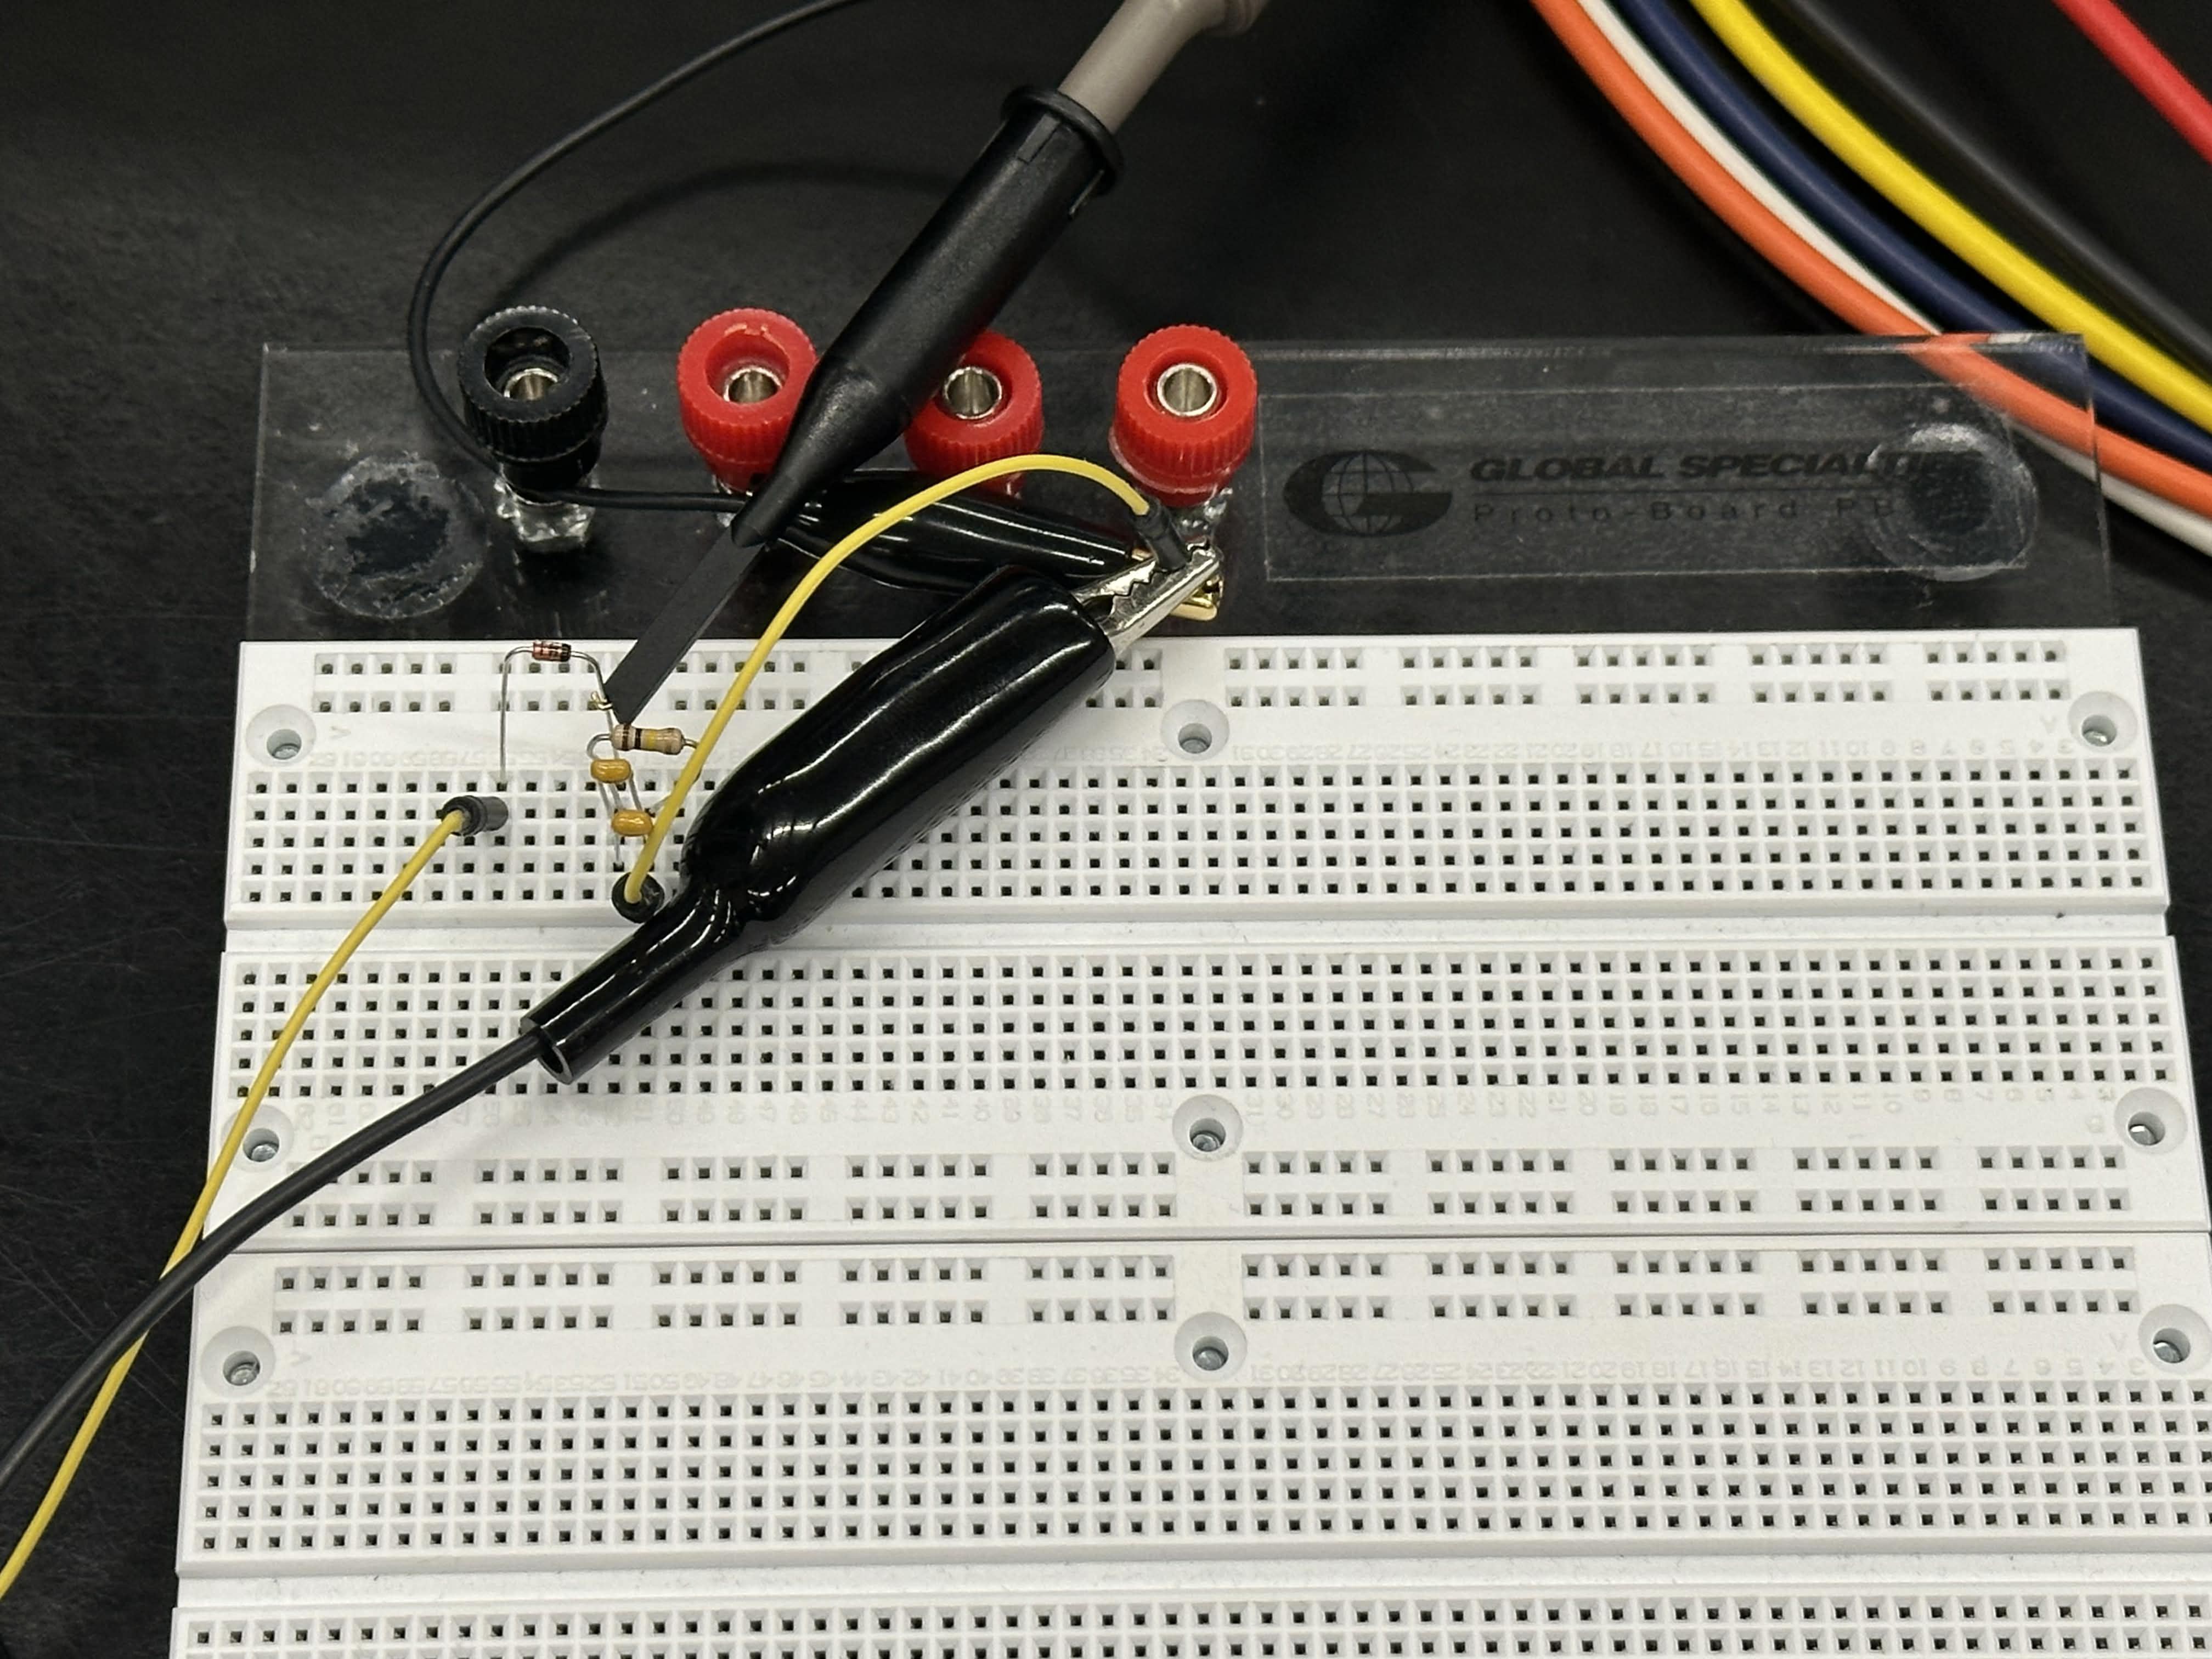
\includegraphics[width=0.5\textwidth]{figure1.jpg}
	\caption{Breadboard of the half-wave rectifier circuit.}
	\label{fig:hand_drawn_1}
\end{figure}

\begin{figure}[H]
	\centering
	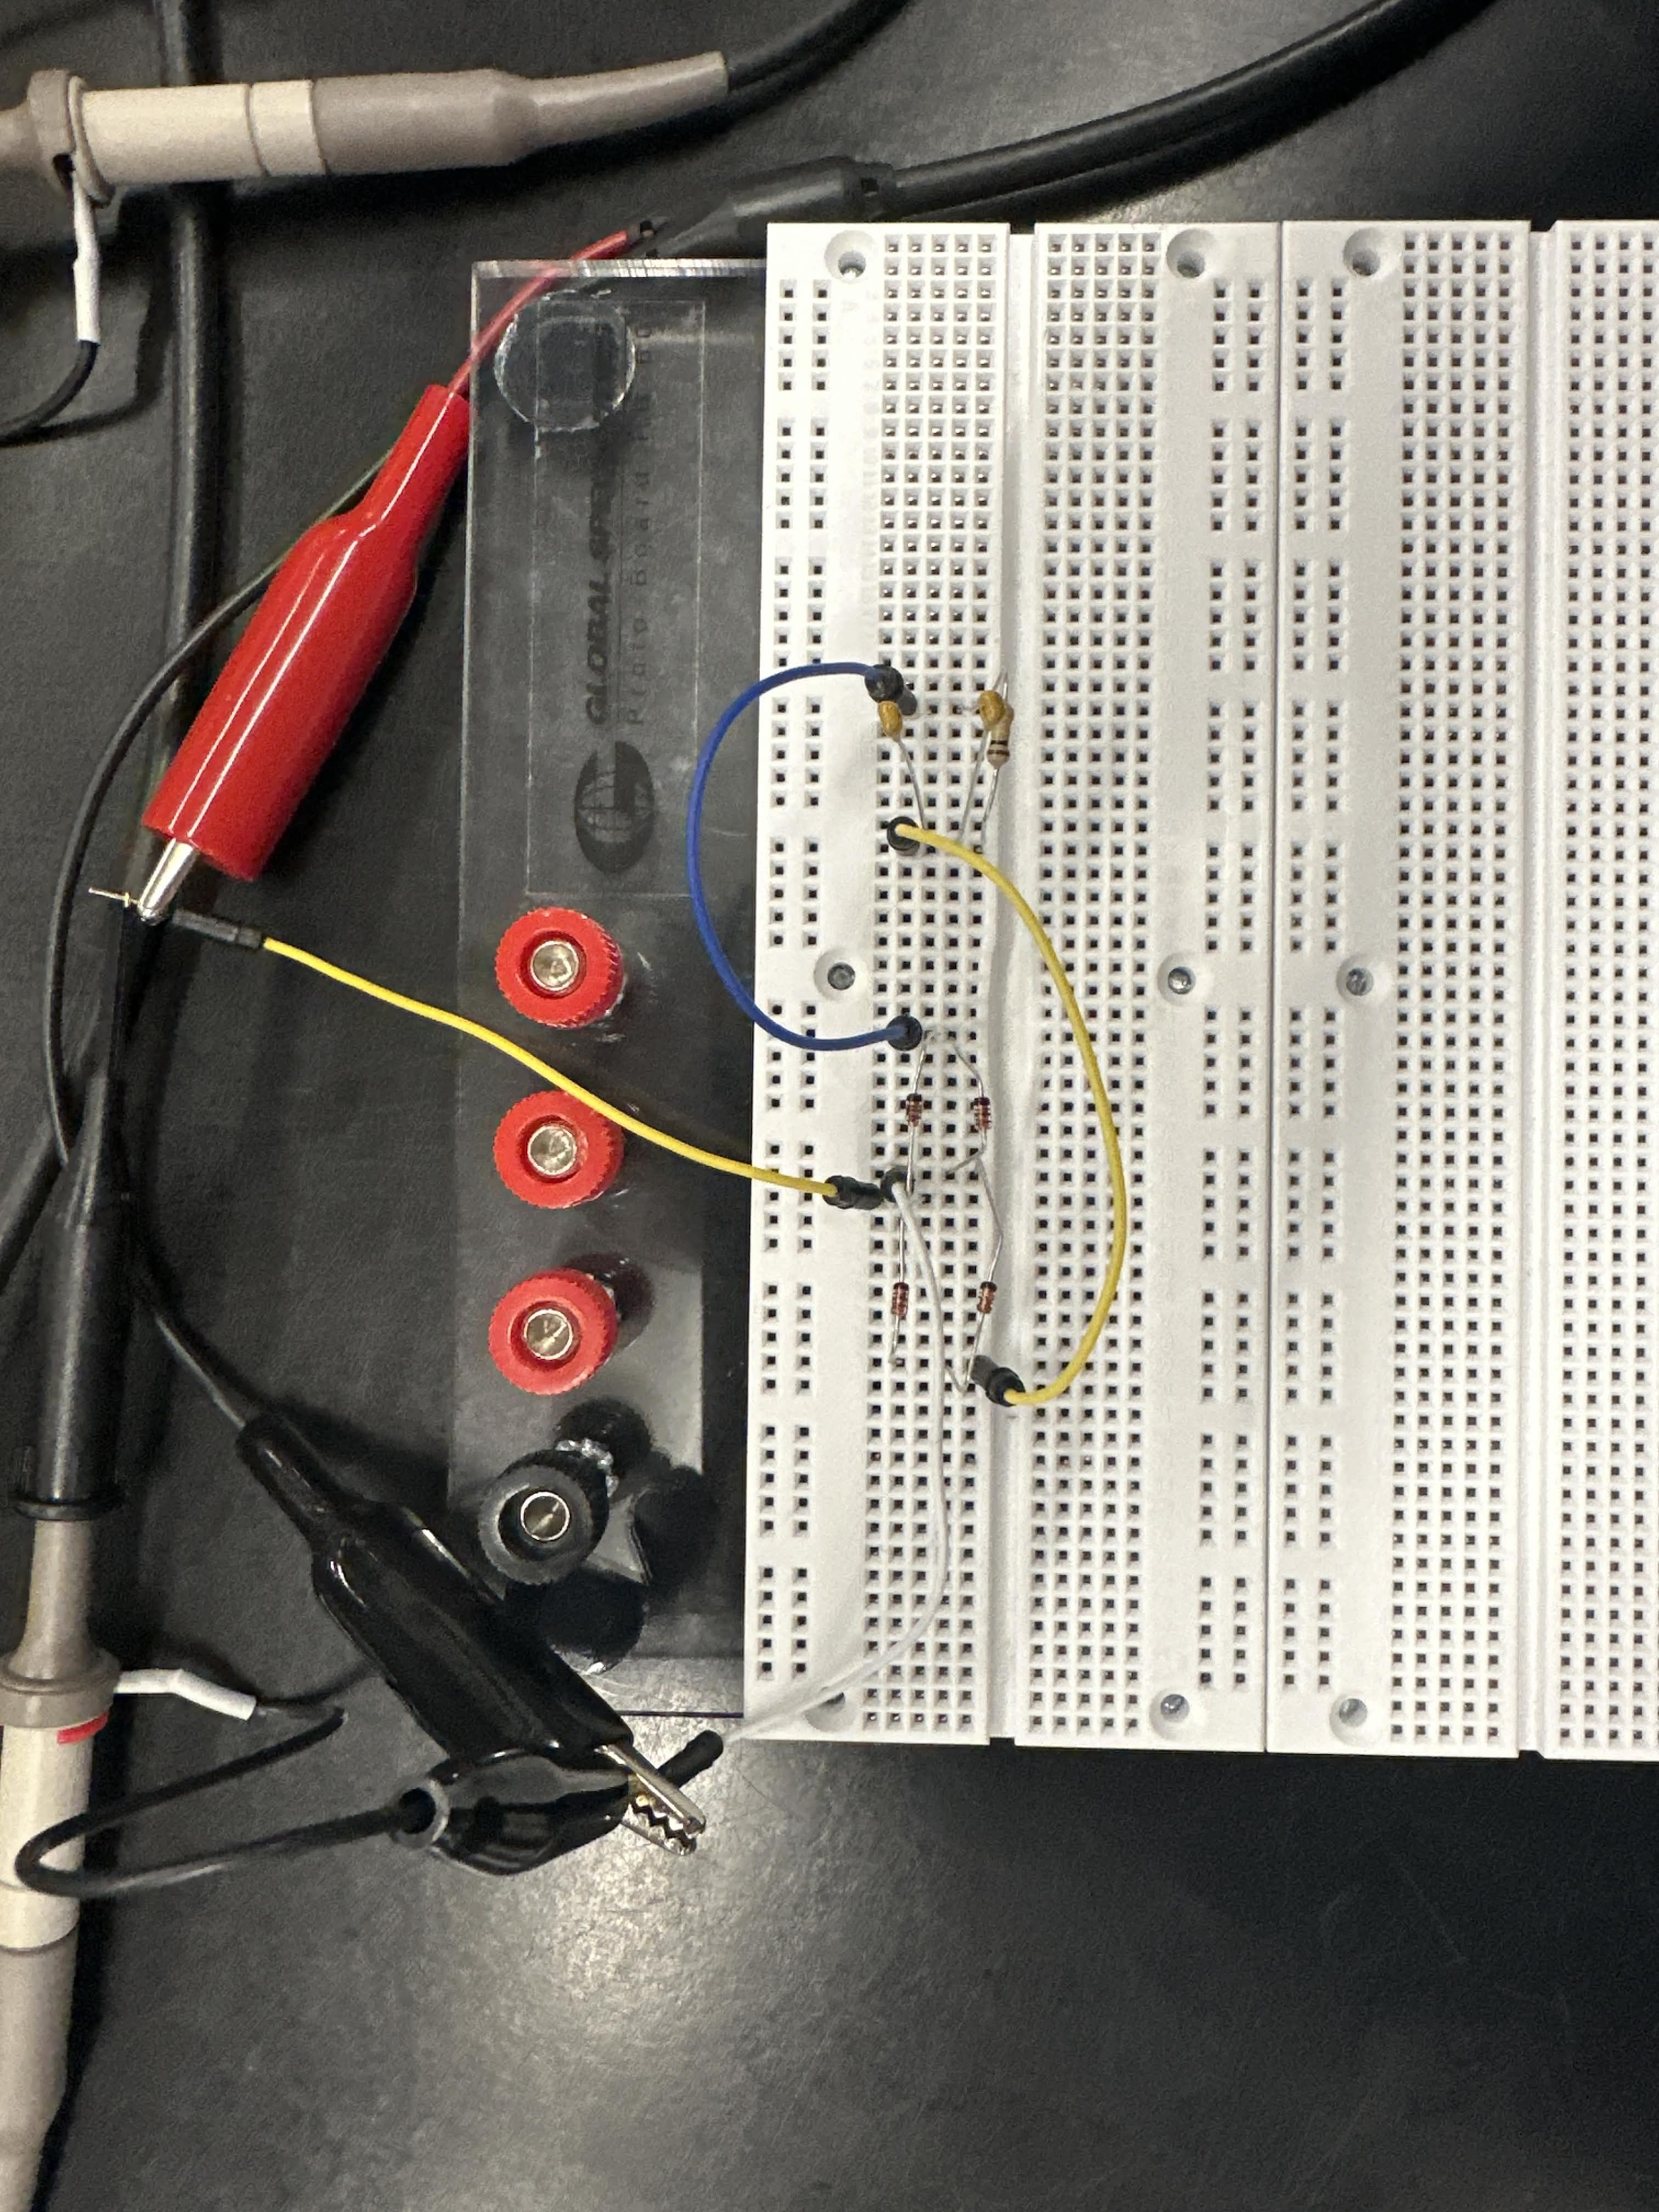
\includegraphics[width=0.5\textwidth, angle=-90]{figure2.jpg}
	\caption{Breadboard of the full-wave rectifier circuit.}
	\label{fig:hand_drawn_2}
\end{figure}

For the half-wave and full-wave rectifier circuits, the experiment was conducted in three parts by selectively shorting or removing components to isolate specific behaviors:
\begin{itemize}
	\item \textbf{Part A (No Capacitor):} The capacitor was removed to create a rectifier.
	\item \textbf{Part B (No Resistor):} The resistor was removed to create a clamping circuit.
	\item \textbf{Part C (Complete Circuit):} All components were included to observe peak rectification and ripple filtering.
\end{itemize}
Additionally, the clipping circuit (Lab Manual Fig.~3), the Zener clipping circuit (Lab Manual Fig.~4), and the clamping circuit (Lab Manual Fig.~5) were each built and tested separately.

\pagebreak
%----------------------------------------------------------------------------------------
%	PRE-LABORATORY CALCULATIONS
%----------------------------------------------------------------------------------------
\section{Pre-Laboratory Calculations}
The following calculations were performed prior to the experiment using the component values and conditions specified in the lab manual.

\subsection{Component Selection}
The lab manual requires the RC time constant $\tau = R_L C \approx 0.2\,\text{s}$. The selected values were:
\[
R_L = 20\,\text{k}\Omega, \quad C = 10\,\mu\text{F}
\quad \Rightarrow \quad
\tau = R_L C = (20 \times 10^{3})(10 \times 10^{-6}) = 0.2\,\text{s}
\]
The input signal for the rectifier circuits was a sinusoid of frequency $f = 100\,\text{Hz}$ and $10\,\text{V}$ peak-to-peak ($V_p = 5\,\text{V}$).

\subsection{Transfer Characteristics --- Half-Wave Rectifier (No Capacitor)}
With the capacitor removed, the half-wave rectifier reduces to a series resistor--diode circuit. The ideal transfer characteristic is piecewise linear:
\[
V_{out} =
\begin{cases}
V_{in} - V_{on} & \text{if } V_{in} > V_{on} \approx 0.7\,\text{V} \\
0 & \text{if } V_{in} \leq V_{on}
\end{cases}
\]
For $V_{in} > 0.7\,\text{V}$, the output follows a unity-slope line offset by the diode drop. For $V_{in} \leq 0.7\,\text{V}$, the output is zero.

\subsection{Transfer Characteristics --- Full-Wave Rectifier (No Capacitor)}
The full-wave rectifier utilizes both halves of the input cycle:
\[
V_{out} =
\begin{cases}
|V_{in}| - V_{on} & \text{if } |V_{in}| > V_{on} \\
0 & \text{if } |V_{in}| \leq V_{on}
\end{cases}
\]
The resulting transfer curve is a V-shaped function centered at the origin, with dead zones near $\pm V_{on}$.

\subsection{Peak-to-Peak Ripple Voltage Calculation}
For the complete R-C-Diode peak rectifier, the peak-to-peak ripple voltage is approximated by:
\[
V_{r(pp)} \approx \frac{V_p - V_{on}}{f_r \cdot R_L \cdot C}
\]
where $f_r$ is the ripple frequency and $(V_p - V_{on})$ is the peak output voltage.

\textbf{Half-wave rectifier} ($f_r = f = 100\,\text{Hz}$):
\[
V_{r(pp)} \approx \frac{5.0 - 0.7}{100 \times 0.2} = \frac{4.3}{20} = 0.215\,\text{V}
\]

\textbf{Full-wave rectifier} ($f_r = 2f = 200\,\text{Hz}$):
\[
V_{r(pp)} \approx \frac{4.3}{200 \times 0.2} = \frac{4.3}{40} = 0.1075\,\text{V}
\]
The full-wave configuration reduces the ripple by approximately a factor of two, consistent with the doubled charging frequency.

\subsection{Clipping Circuit Transfer Characteristics}
\textbf{Standard Clipper (Fig.~3):}
The output tracks the input until the input exceeds the clipping threshold:
\[
V_{out} =
\begin{cases}
V_{in} & \text{if } V_{in} < V_{ref} + V_{on} \\
V_{ref} + V_{on} & \text{if } V_{in} \geq V_{ref} + V_{on}
\end{cases}
\]

\textbf{Zener Clipper (Fig.~4):}
With two back-to-back 1N5234 Zener diodes ($V_Z \approx 6.2\,\text{V}$), the output is symmetrically clipped:
\[
V_{out} =
\begin{cases}
+(V_Z + V_{on}) \approx +6.85\,\text{V} & \text{if } V_{in} > +(V_Z + V_{on}) \\
V_{in} & \text{if } |V_{in}| < (V_Z + V_{on}) \\
-(V_Z + V_{on}) \approx -6.85\,\text{V} & \text{if } V_{in} < -(V_Z + V_{on})
\end{cases}
\]

\subsection{Clamping Circuit Pre-Lab Analysis (Fig.~5)}
For a sinusoidal input of amplitude $V_p$, the capacitor charges through the forward-biased diode during the first negative half-cycle to approximately $V_p - V_{on}$. The output is the superposition of the input and this stored DC voltage:
\[
V_{out}(t) = V_{in}(t) + (V_p - V_{on})
\]
Therefore, the output extremes are:
\begin{align*}
V_{out,\text{max}} &= V_p + (V_p - V_{on}) = 2V_p - V_{on} \\
V_{out,\text{min}} &= -V_p + (V_p - V_{on}) = -V_{on} \approx -0.65\,\text{V}
\end{align*}
The entire waveform is shifted so that its most negative excursion is clamped near $-V_{on}$.

\pagebreak
%----------------------------------------------------------------------------------------
%	3. RESULTS AND DISCUSSION
%----------------------------------------------------------------------------------------
\section{Results and Discussion}

%-----------------------------------------
% PART A: Rectifier
%-----------------------------------------
\subsection{Half-Wave Rectifier (Lab Manual Fig.~1)}
\subsubsection{Part A: No Capacitor (Resistor-Diode Circuit)}
In this configuration, the capacitor was removed. The diode was placed in series with the source and the load resistor. The LTspice schematic for this setup is shown in Figure \ref{fig:sch_rect}.

\begin{figure}[H]
	\centering
	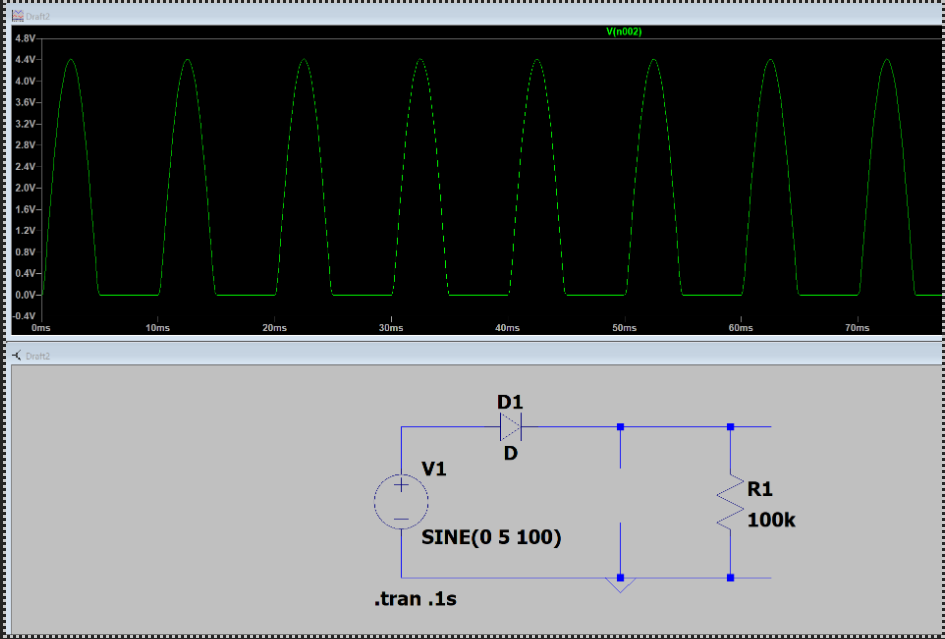
\includegraphics[width=0.6\textwidth]{figure1_nocapacitor_ltspice.png}
	\caption{LTspice simulation schematic for the Half-Wave Rectifier (No Capacitor).}
	\label{fig:sch_rect}
\end{figure}

Experimental waveforms for sinusoidal and square wave inputs were captured and are presented in Figure~\ref{fig:rect_results}.

\begin{figure}[H]
	\centering
	\begin{subfigure}[b]{0.48\textwidth}
		\centering
		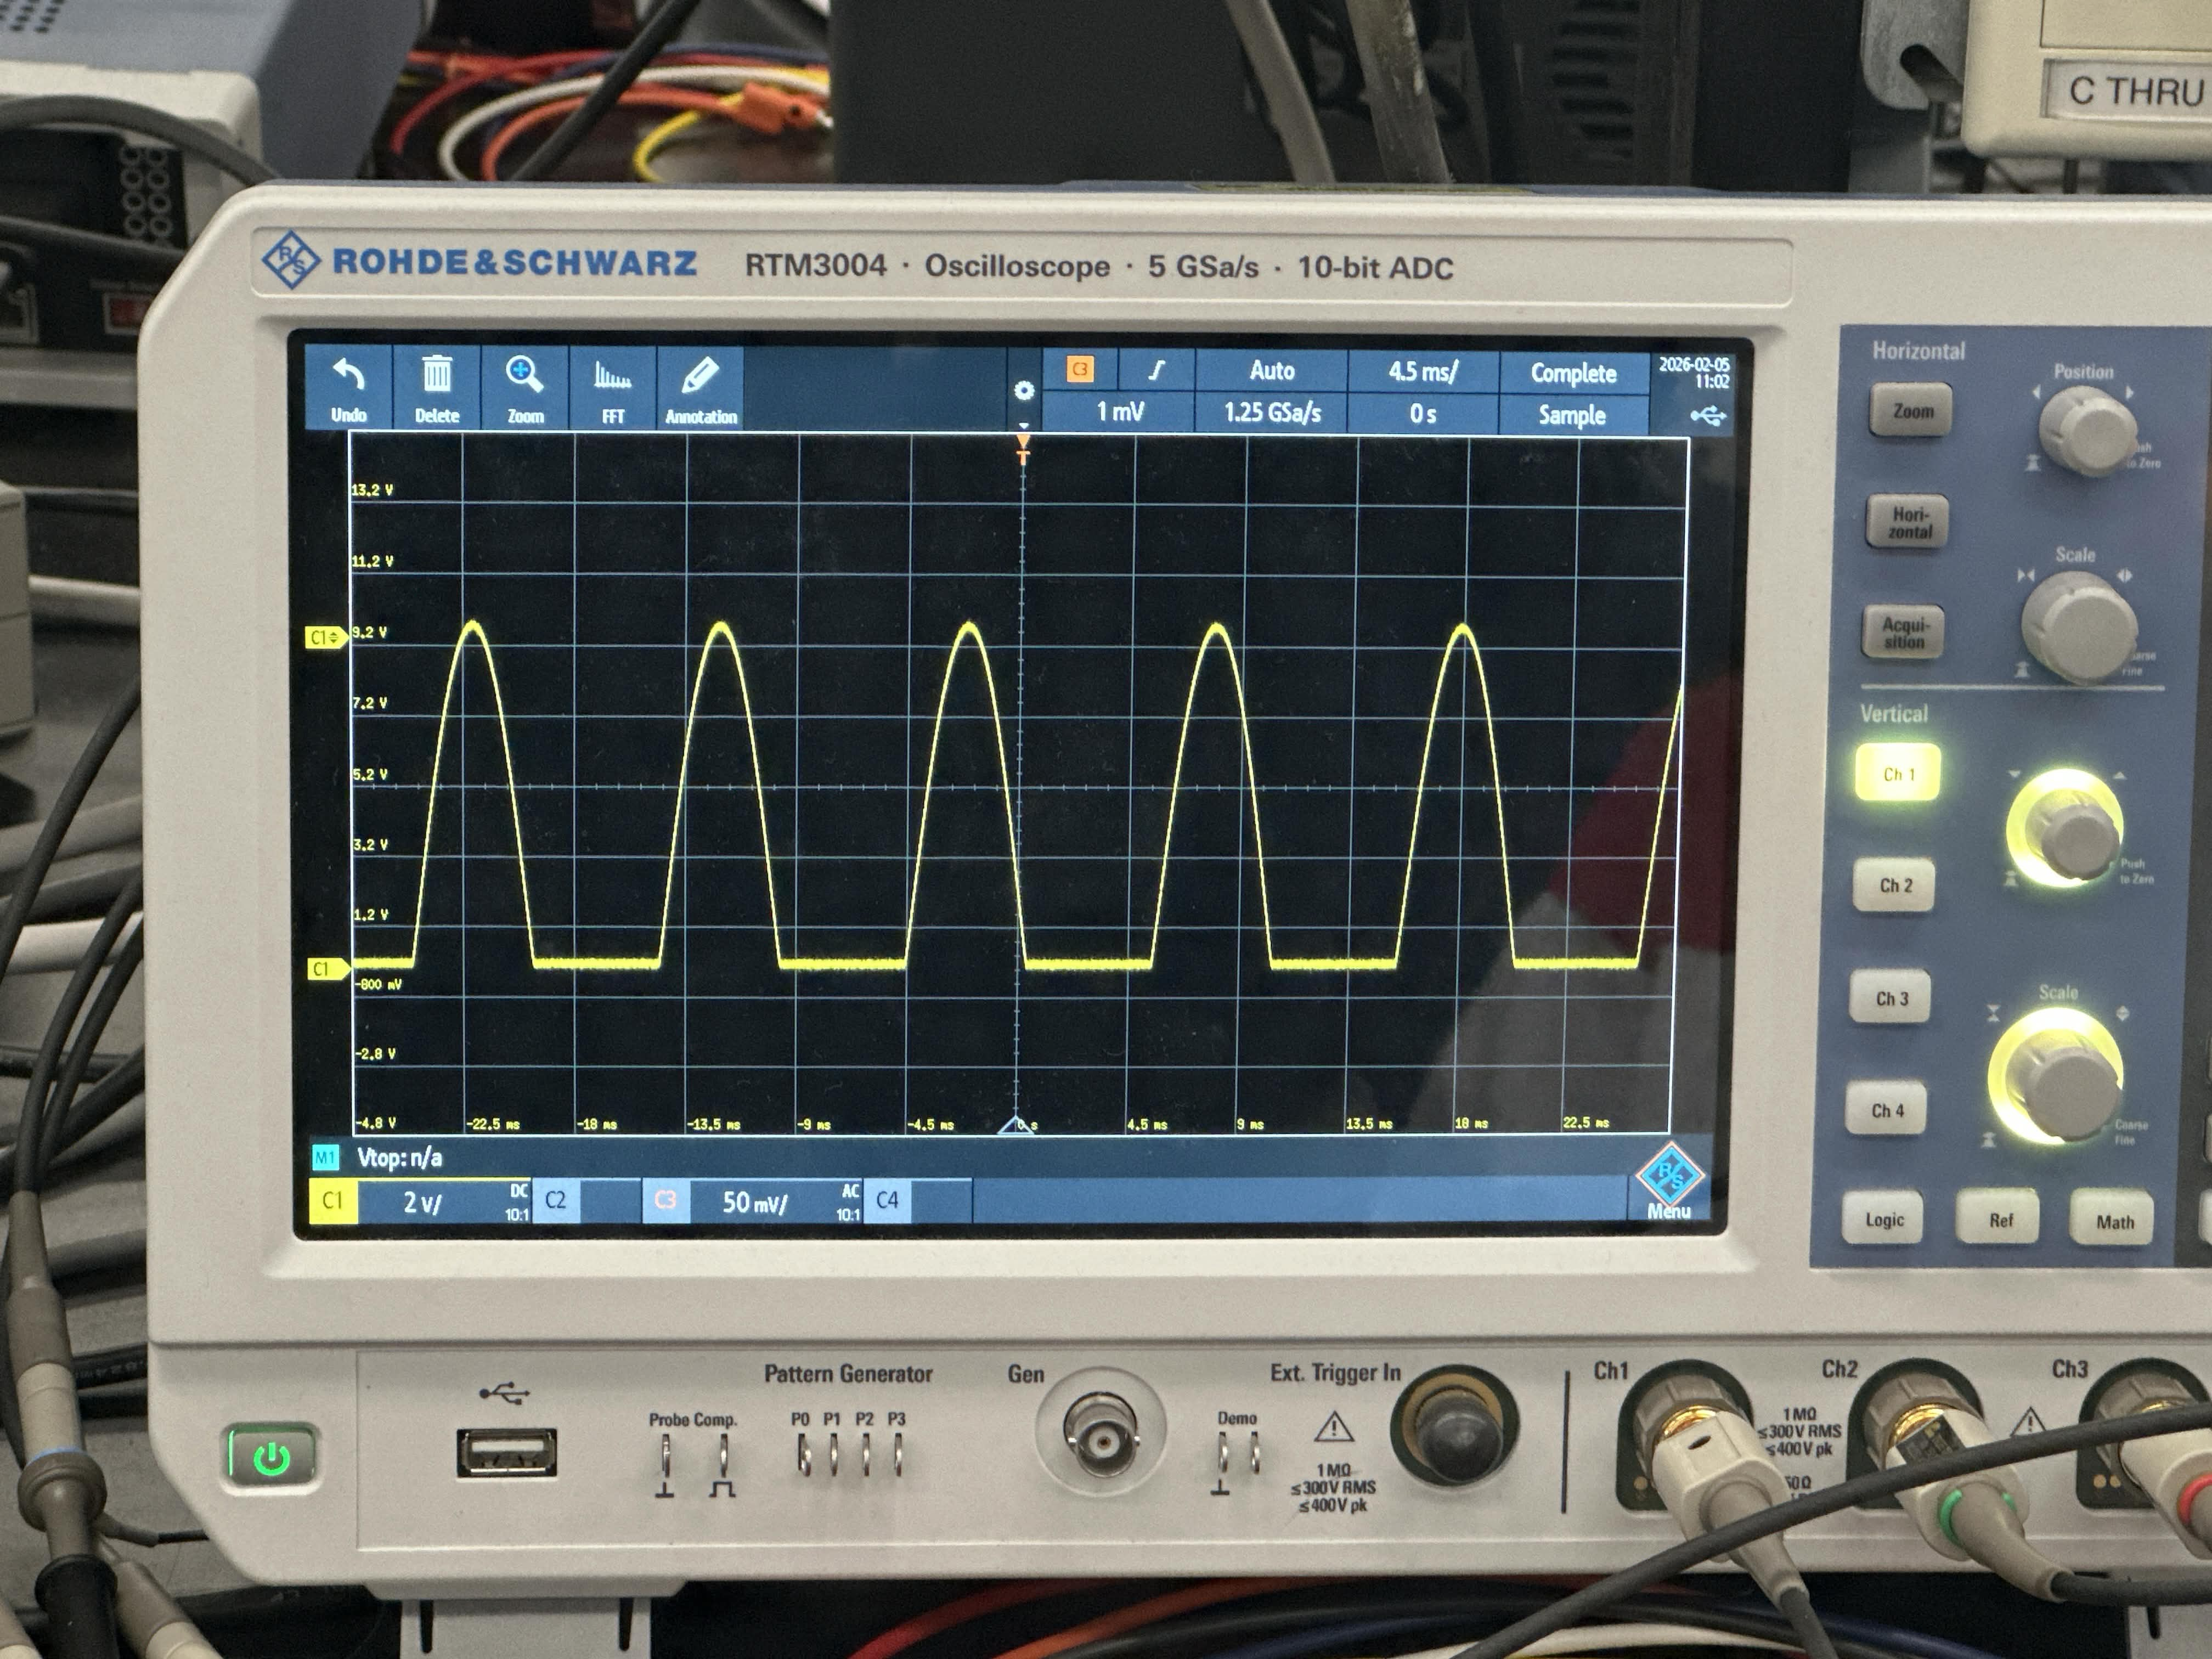
\includegraphics[width=\textwidth]{figure1_nocapacitor_sine.jpg}
		\caption{Sinusoidal Input (Blue) vs Output (Yellow)}
		\label{fig:rect_sine}
	\end{subfigure}
	\hfill
	\begin{subfigure}[b]{0.48\textwidth}
		\centering
		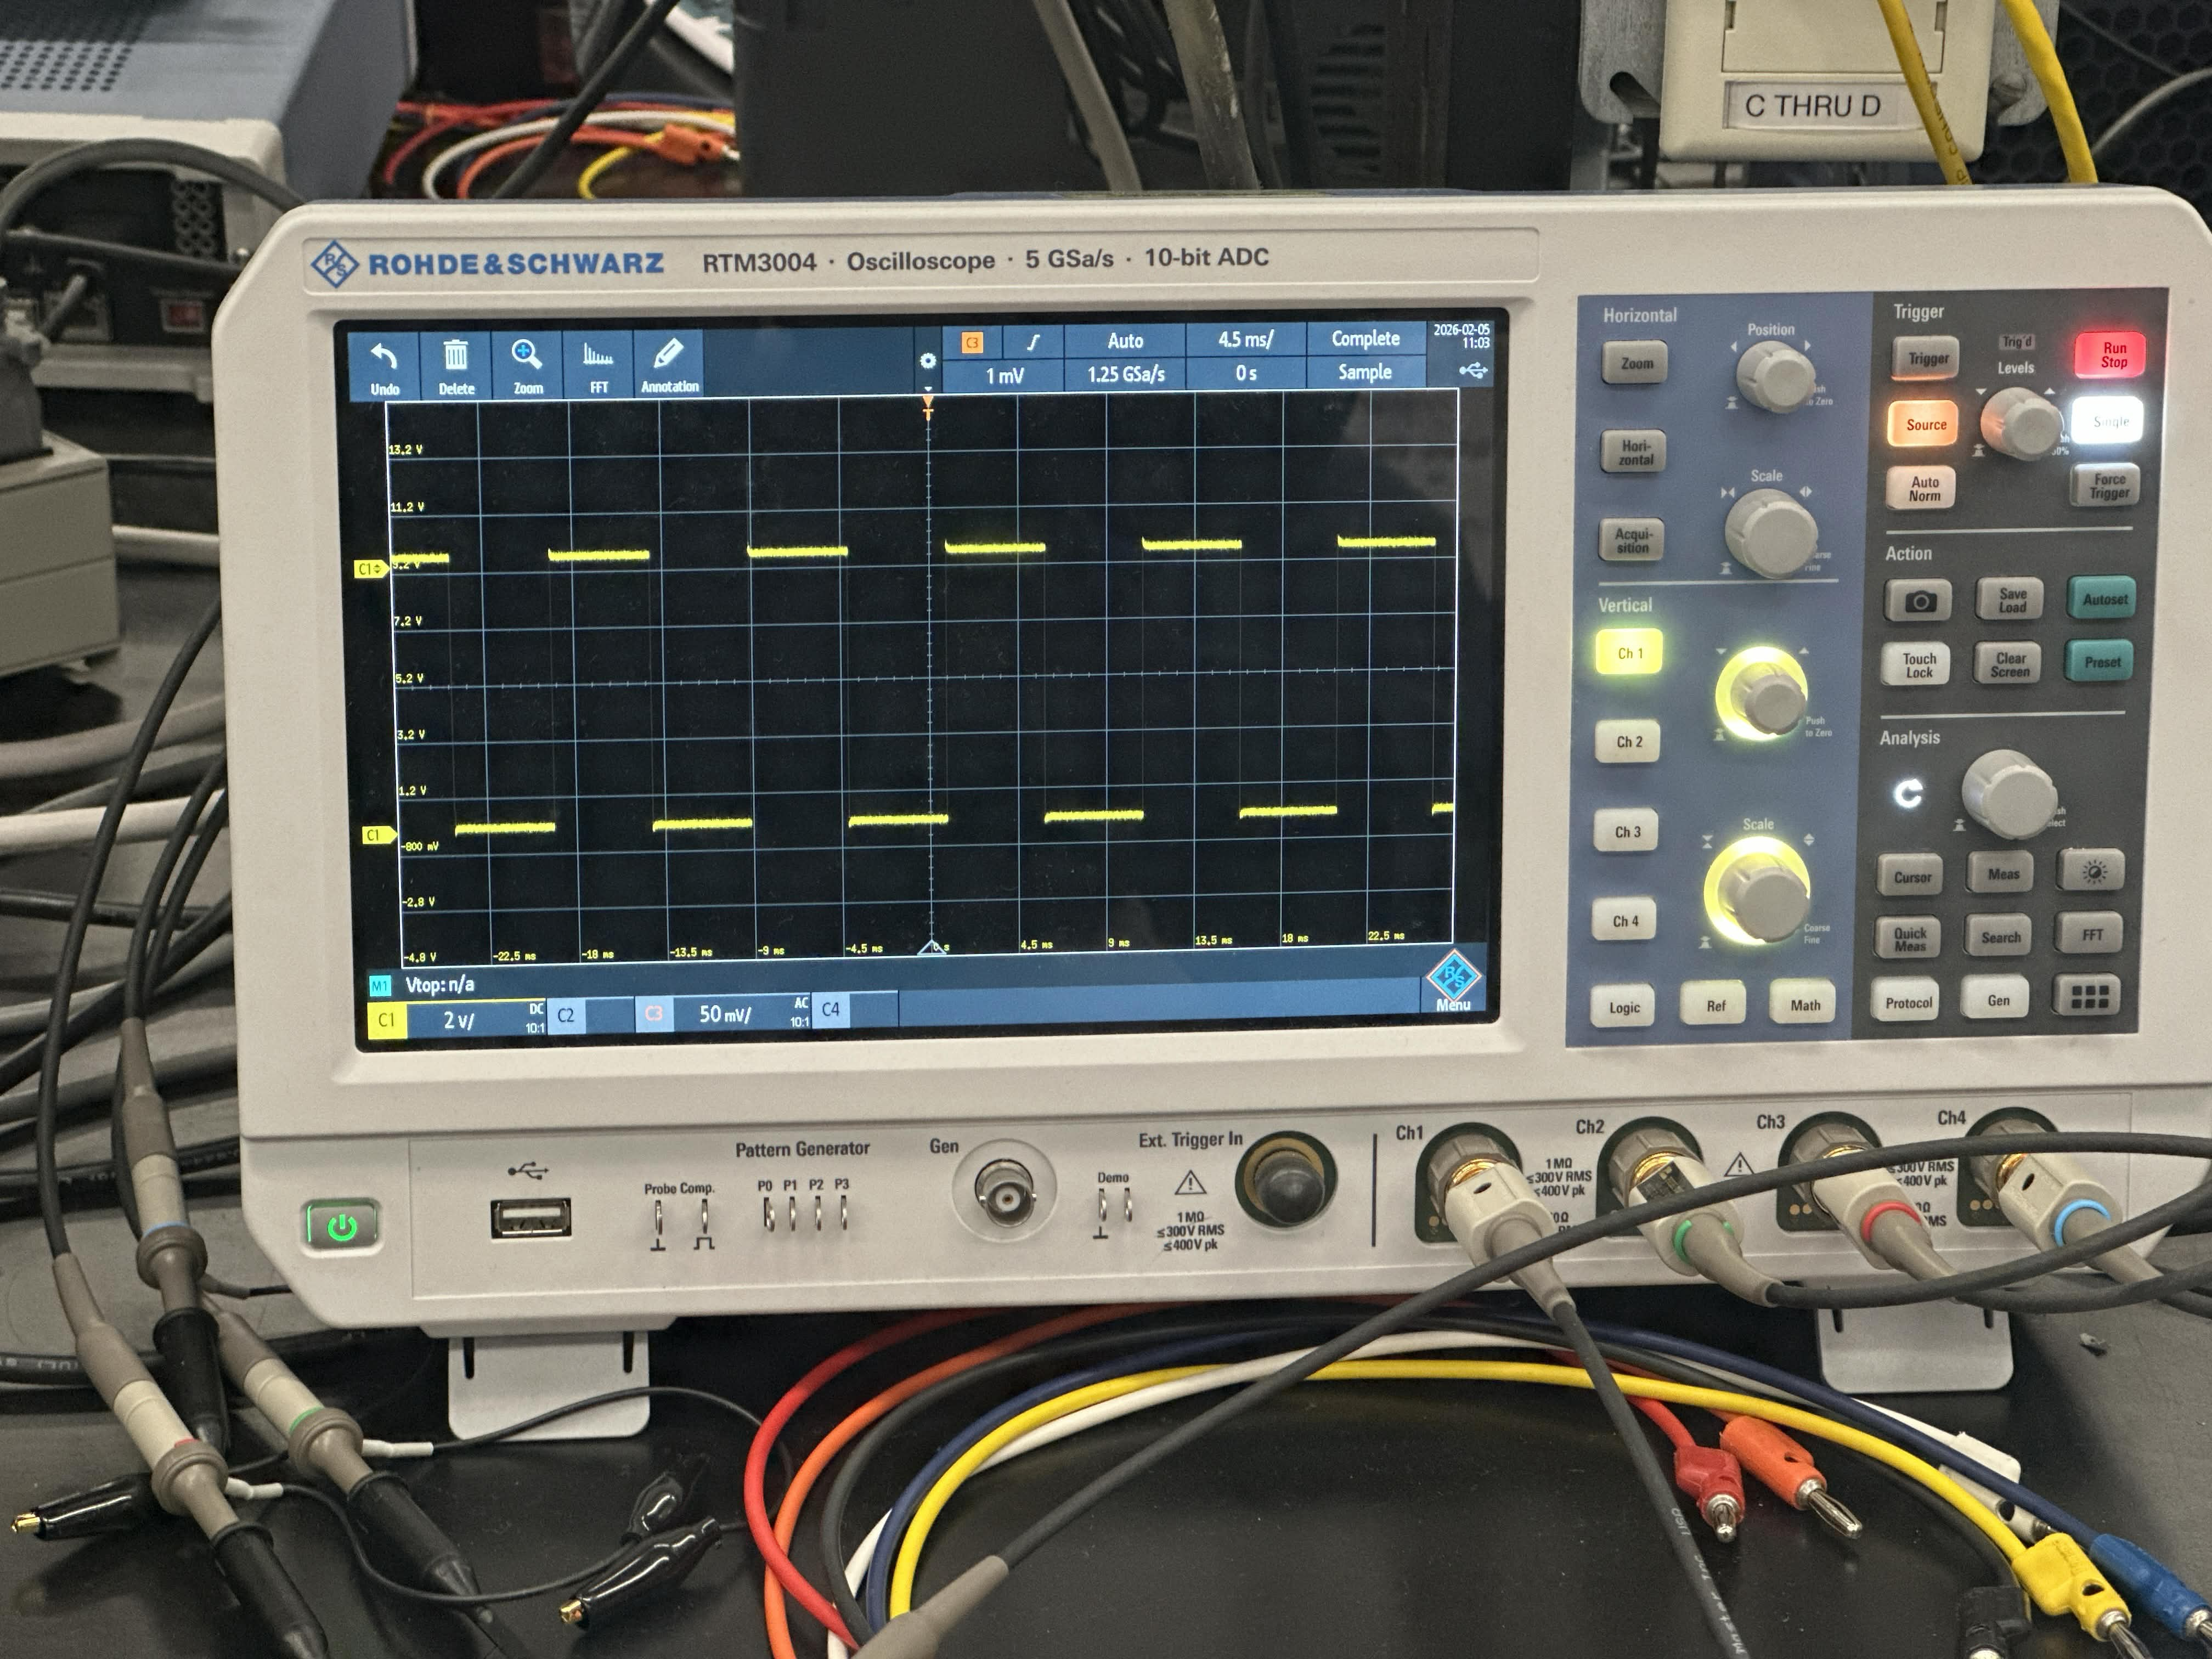
\includegraphics[width=\textwidth]{figure1_nocapacitor_square.jpg}
		\caption{Square Input (Blue) vs Output (Yellow)}
		\label{fig:rect_square}
	\end{subfigure}
	\caption{Oscilloscope captures for the Resistor-Diode Half-Wave Rectifier.}
	\label{fig:rect_results}
\end{figure}

\textbf{Discussion:} \\
As observed in Figure \ref{fig:rect_sine}, the circuit functions as a positive half-wave rectifier.
\begin{itemize}
	\item \textbf{Forward Bias:} During the positive half-cycle of the input (Blue trace), the diode is forward-biased and conducts current. The output voltage (Yellow trace) follows the input voltage.
	\item \textbf{Diode Voltage Drop:} A voltage difference is visible between the peak of the input and the peak of the output. The output peak is approximately $0.6V$ to $0.7V$ lower than the input peak, corresponding to the built-in potential barrier ($V_{on}$) of the silicon diode.
	\item \textbf{Reverse Bias:} During the negative half-cycle, the diode is reverse-biased (acting as an open switch). No current flows through the resistor, resulting in an output voltage of $0V$.
\end{itemize}

\textbf{Calculation:}
For a $10\,\text{V}_{pp}$ input ($V_p = 5\,\text{V}$), the theoretical peak output voltage is:
\[
V_{out,peak} = V_p - V_{on} = 5.0 - 0.7 = 4.3\,\text{V}
\]
This matches the transfer characteristic derived in the pre-lab: $V_{out} = V_{in} - V_{on}$ for $V_{in} > V_{on}$, and $V_{out} = 0$ otherwise.

The square wave response in Figure \ref{fig:rect_square} confirms this switching behavior, where the negative portion of the square wave is completely clipped off.

%-----------------------------------------
% PART B: Clamper
%-----------------------------------------
\subsubsection{Part B: No Resistor (Capacitor-Diode Clamper)}
In this section, the resistor was removed, leaving the capacitor in series with the diode. This configuration creates a clamping circuit, which is designed to shift the DC level of the signal.

\begin{figure}[H]
	\centering
	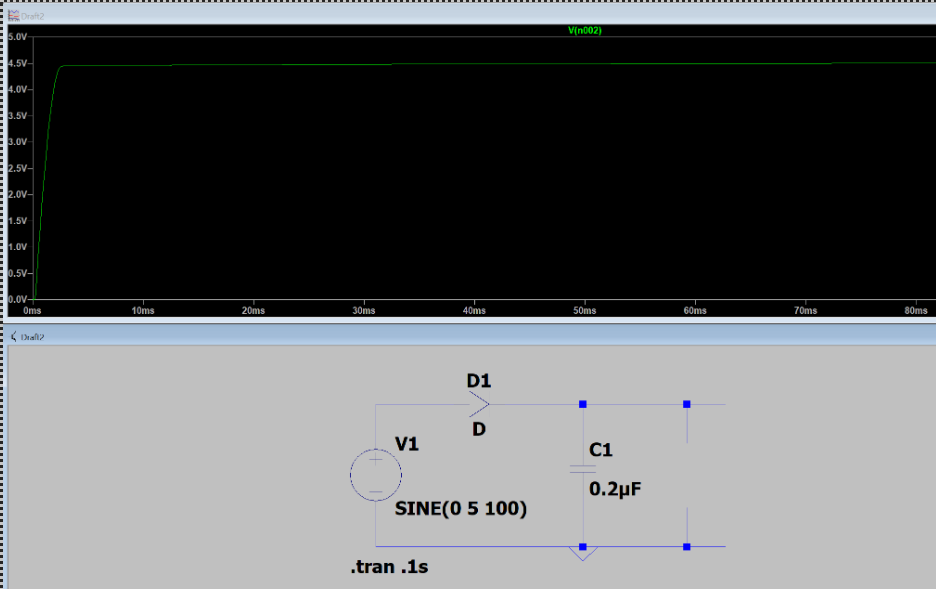
\includegraphics[width=0.6\textwidth]{figure1_noresistor_ltspice.png}
	\caption{LTspice simulation schematic for the Capacitor-Diode Clamper.}
	\label{fig:sch_clamp}
\end{figure}

The experimental results for the clamper circuit are shown in Figure \ref{fig:clamp_results}.

\begin{figure}[H]
	\centering
	\begin{subfigure}[b]{0.48\textwidth}
		\centering
		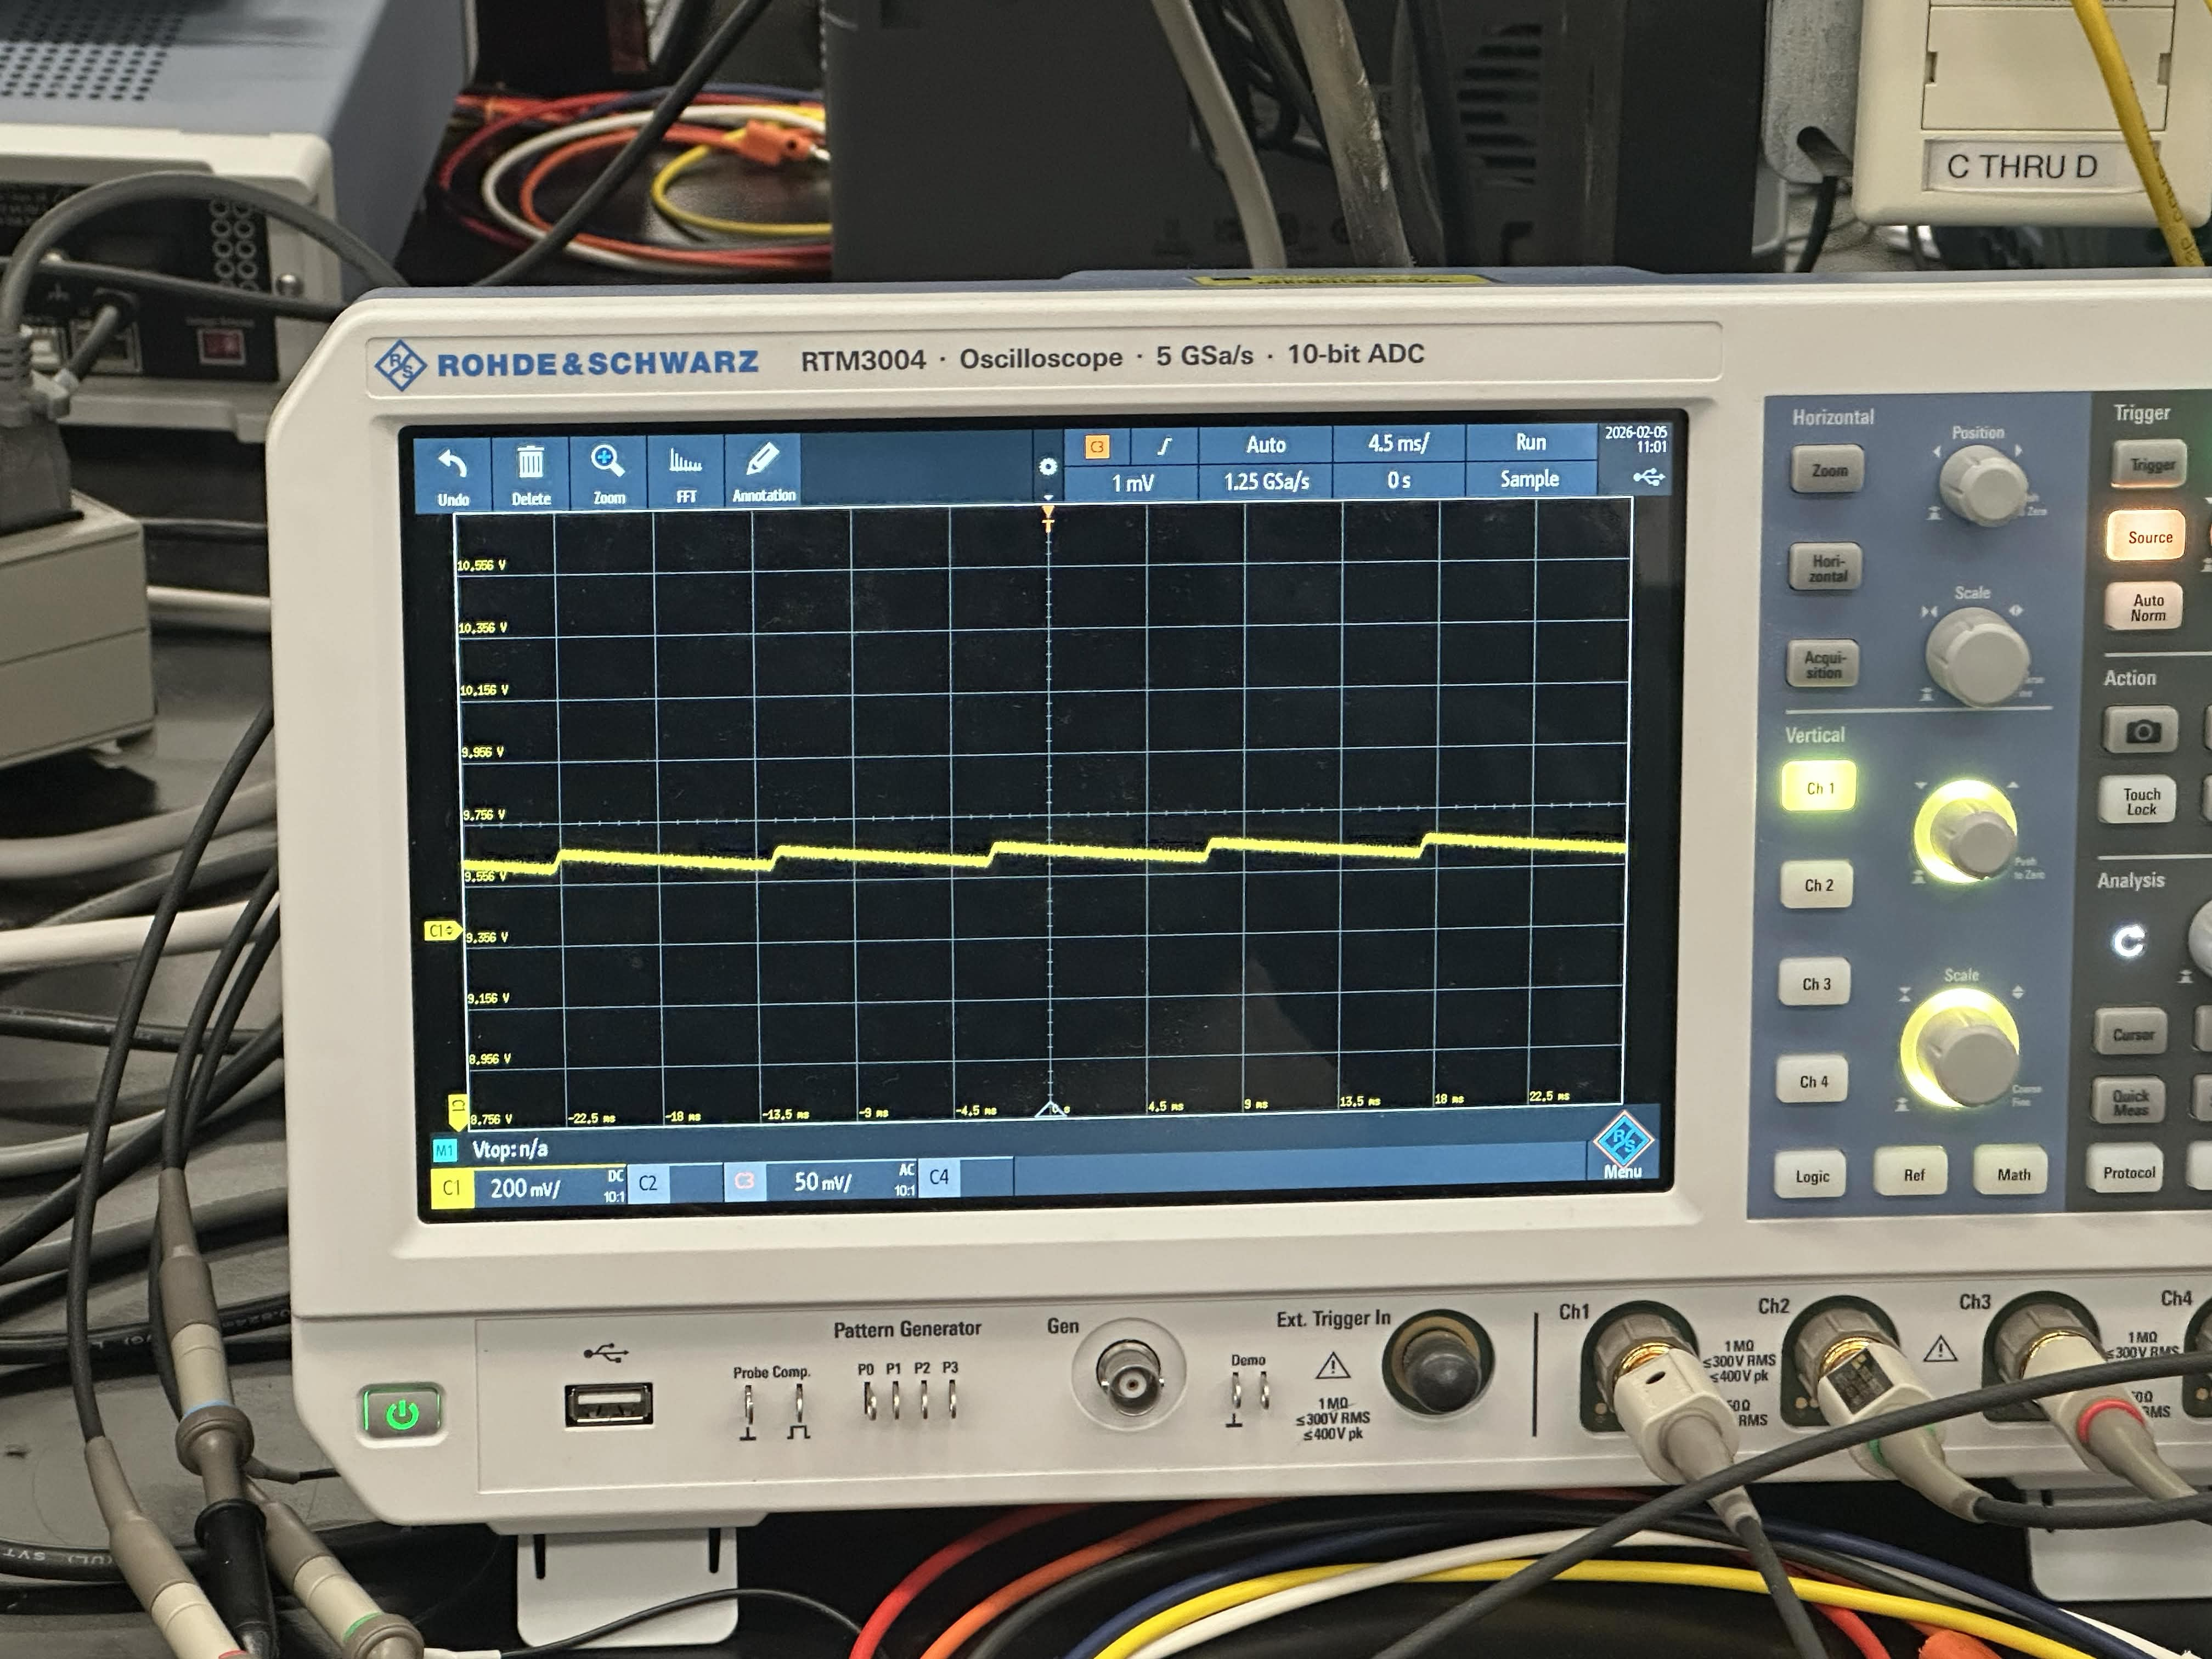
\includegraphics[width=\textwidth]{figure1_noresistor_sine.jpg}
		\caption{Sinusoidal Input (Blue) vs Output (Yellow)}
		\label{fig:clamp_sine}
	\end{subfigure}
	\hfill
	\begin{subfigure}[b]{0.48\textwidth}
		\centering
		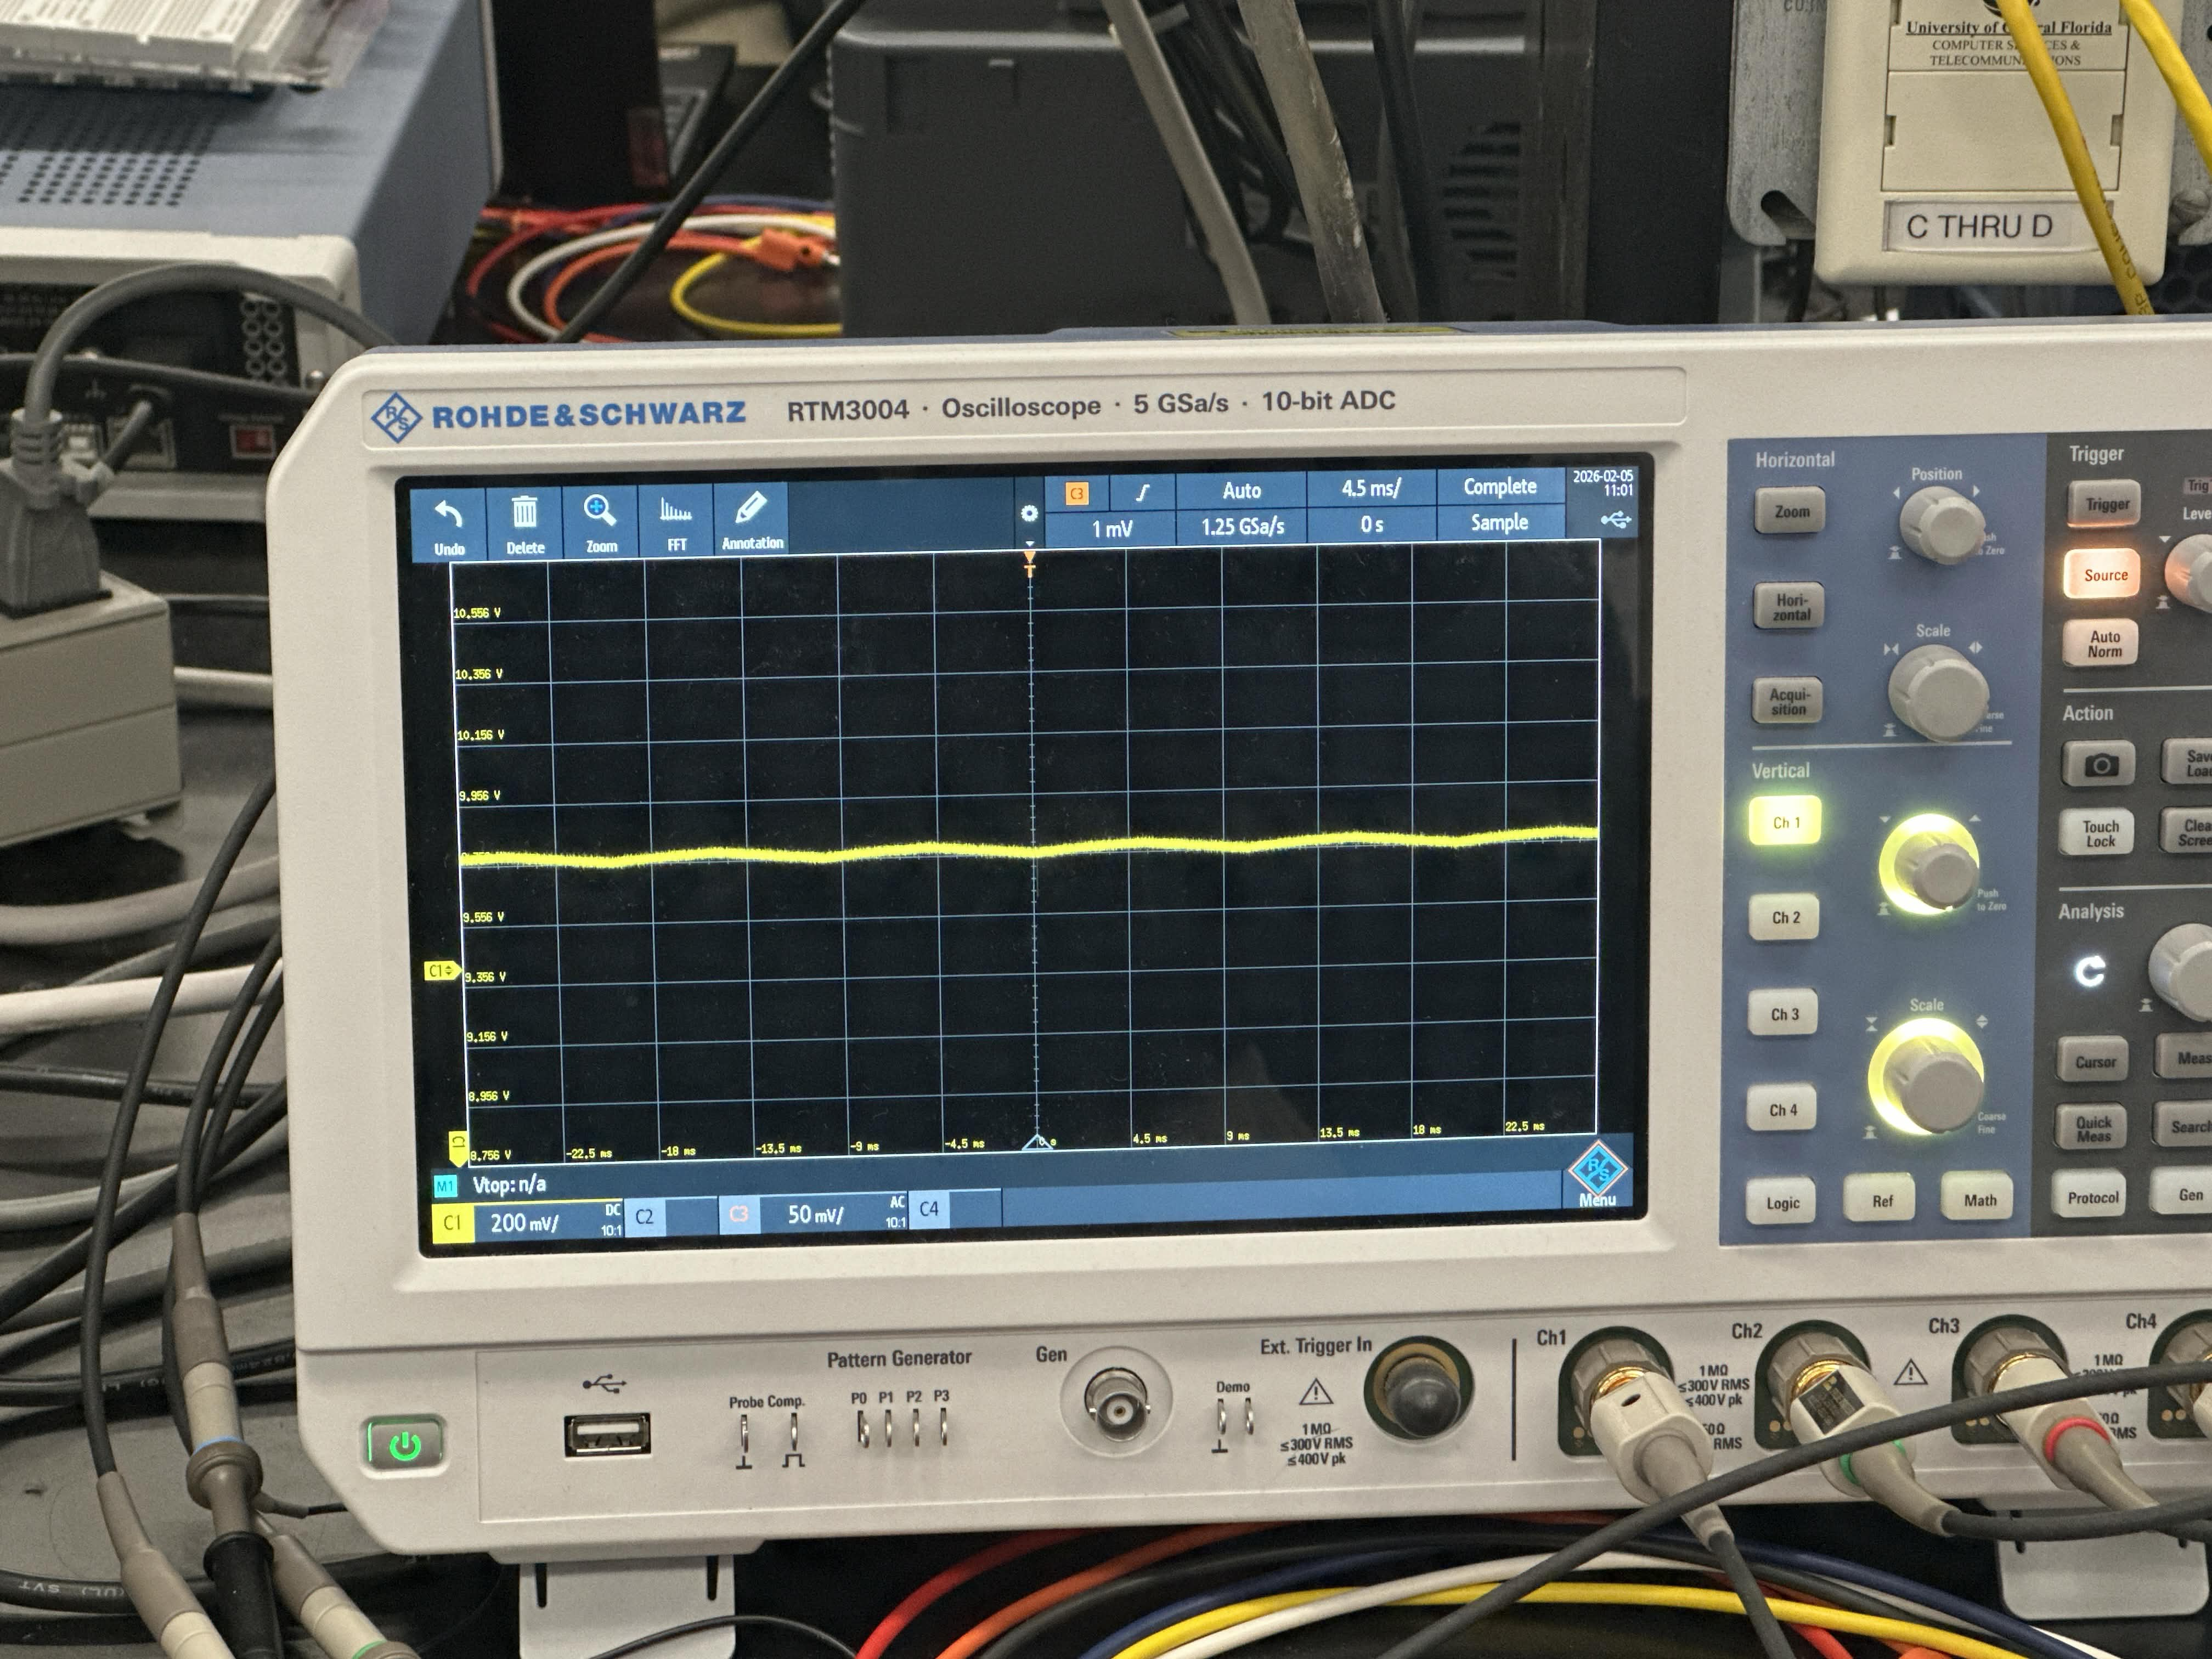
\includegraphics[width=\textwidth]{figure1_noresistor_square.jpg}
		\caption{Square Input (Blue) vs Output (Yellow)}
		\label{fig:clamp_square}
	\end{subfigure}
	\caption{Oscilloscope captures for the Capacitor-Diode Clamping Circuit.}
	\label{fig:clamp_results}
\end{figure}

\textbf{Discussion:} \\
The waveforms in Figure \ref{fig:clamp_results} demonstrate the DC restoring capability of the clamper.
\begin{itemize}
	\item \textbf{DC Shift:} Unlike the rectifier, the clamper does not alter the shape of the waveform; it shifts the entire signal. In Figure \ref{fig:clamp_sine}, the yellow output wave has the same peak-to-peak amplitude as the blue input wave but is shifted downwards (or upwards depending on diode polarity).
	\item \textbf{Capacitor Action:} During the first negative half-cycle (assuming the diode is oriented to conduct then), the capacitor charges to the peak input voltage ($V_p - V_{on}$). Once charged, the capacitor acts like a DC battery in series with the source.
	\item \textbf{Observation:} The output signal appears ``clamped'' such that its peaks (or troughs) are fixed relative to a reference voltage level determined by the diode drop.
\end{itemize}

\textbf{Calculation:}
For a $10\,\text{V}_{pp}$ sinusoidal input ($V_p = 5\,\text{V}$), the capacitor charges to:
\[
V_C = V_p - V_{on} = 5.0 - 0.7 = 4.3\,\text{V}
\]
The expected output range is therefore:
\[
V_{out,\text{min}} = -V_{on} \approx -0.7\,\text{V}, \qquad
V_{out,\text{max}} = 2V_p - V_{on} = 9.3\,\text{V}
\]
The peak-to-peak amplitude of the output ($10\,\text{V}$) matches the input, confirming the shape-preserving DC shift.

%-----------------------------------------
% PART C: Peak Rectifier
%-----------------------------------------
\subsubsection{Part C: Complete R-C-Diode Circuit (Peak Rectifier with Filter)}
The complete circuit includes the resistor, capacitor, and diode. This configuration represents a peak rectifier, commonly used in AC-to-DC power supplies.

\begin{figure}[H]
	\centering
	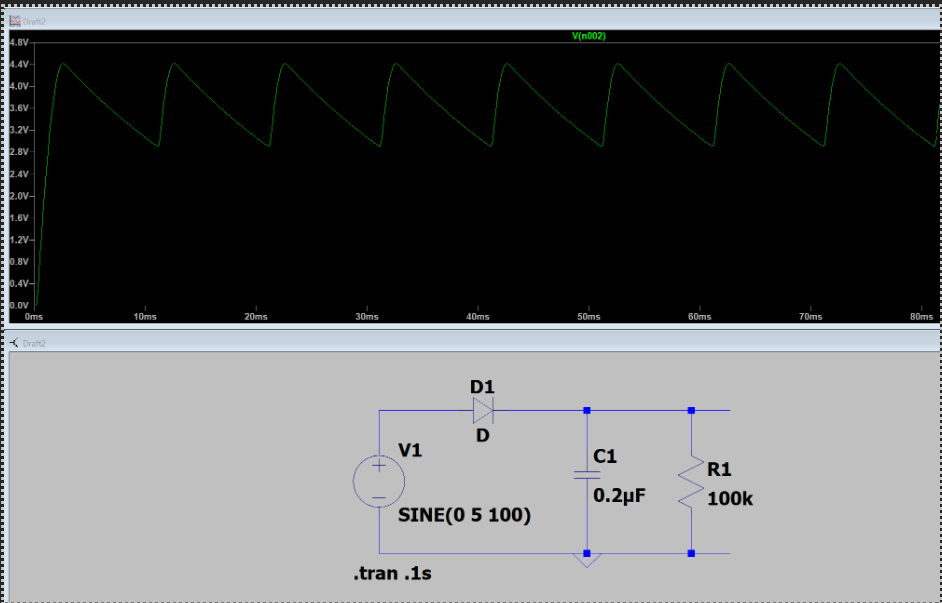
\includegraphics[width=0.6\textwidth]{figure1_all_ltspice.png}
	\caption{LTspice simulation schematic for the complete R-C-Diode Circuit (Half-Wave).}
	\label{fig:sch_all}
\end{figure}

The experimental oscilloscope captures for this configuration are shown in Figure~\ref{fig:hw_all_results}.

\begin{figure}[H]
	\centering
	\begin{subfigure}[b]{0.48\textwidth}
		\centering
		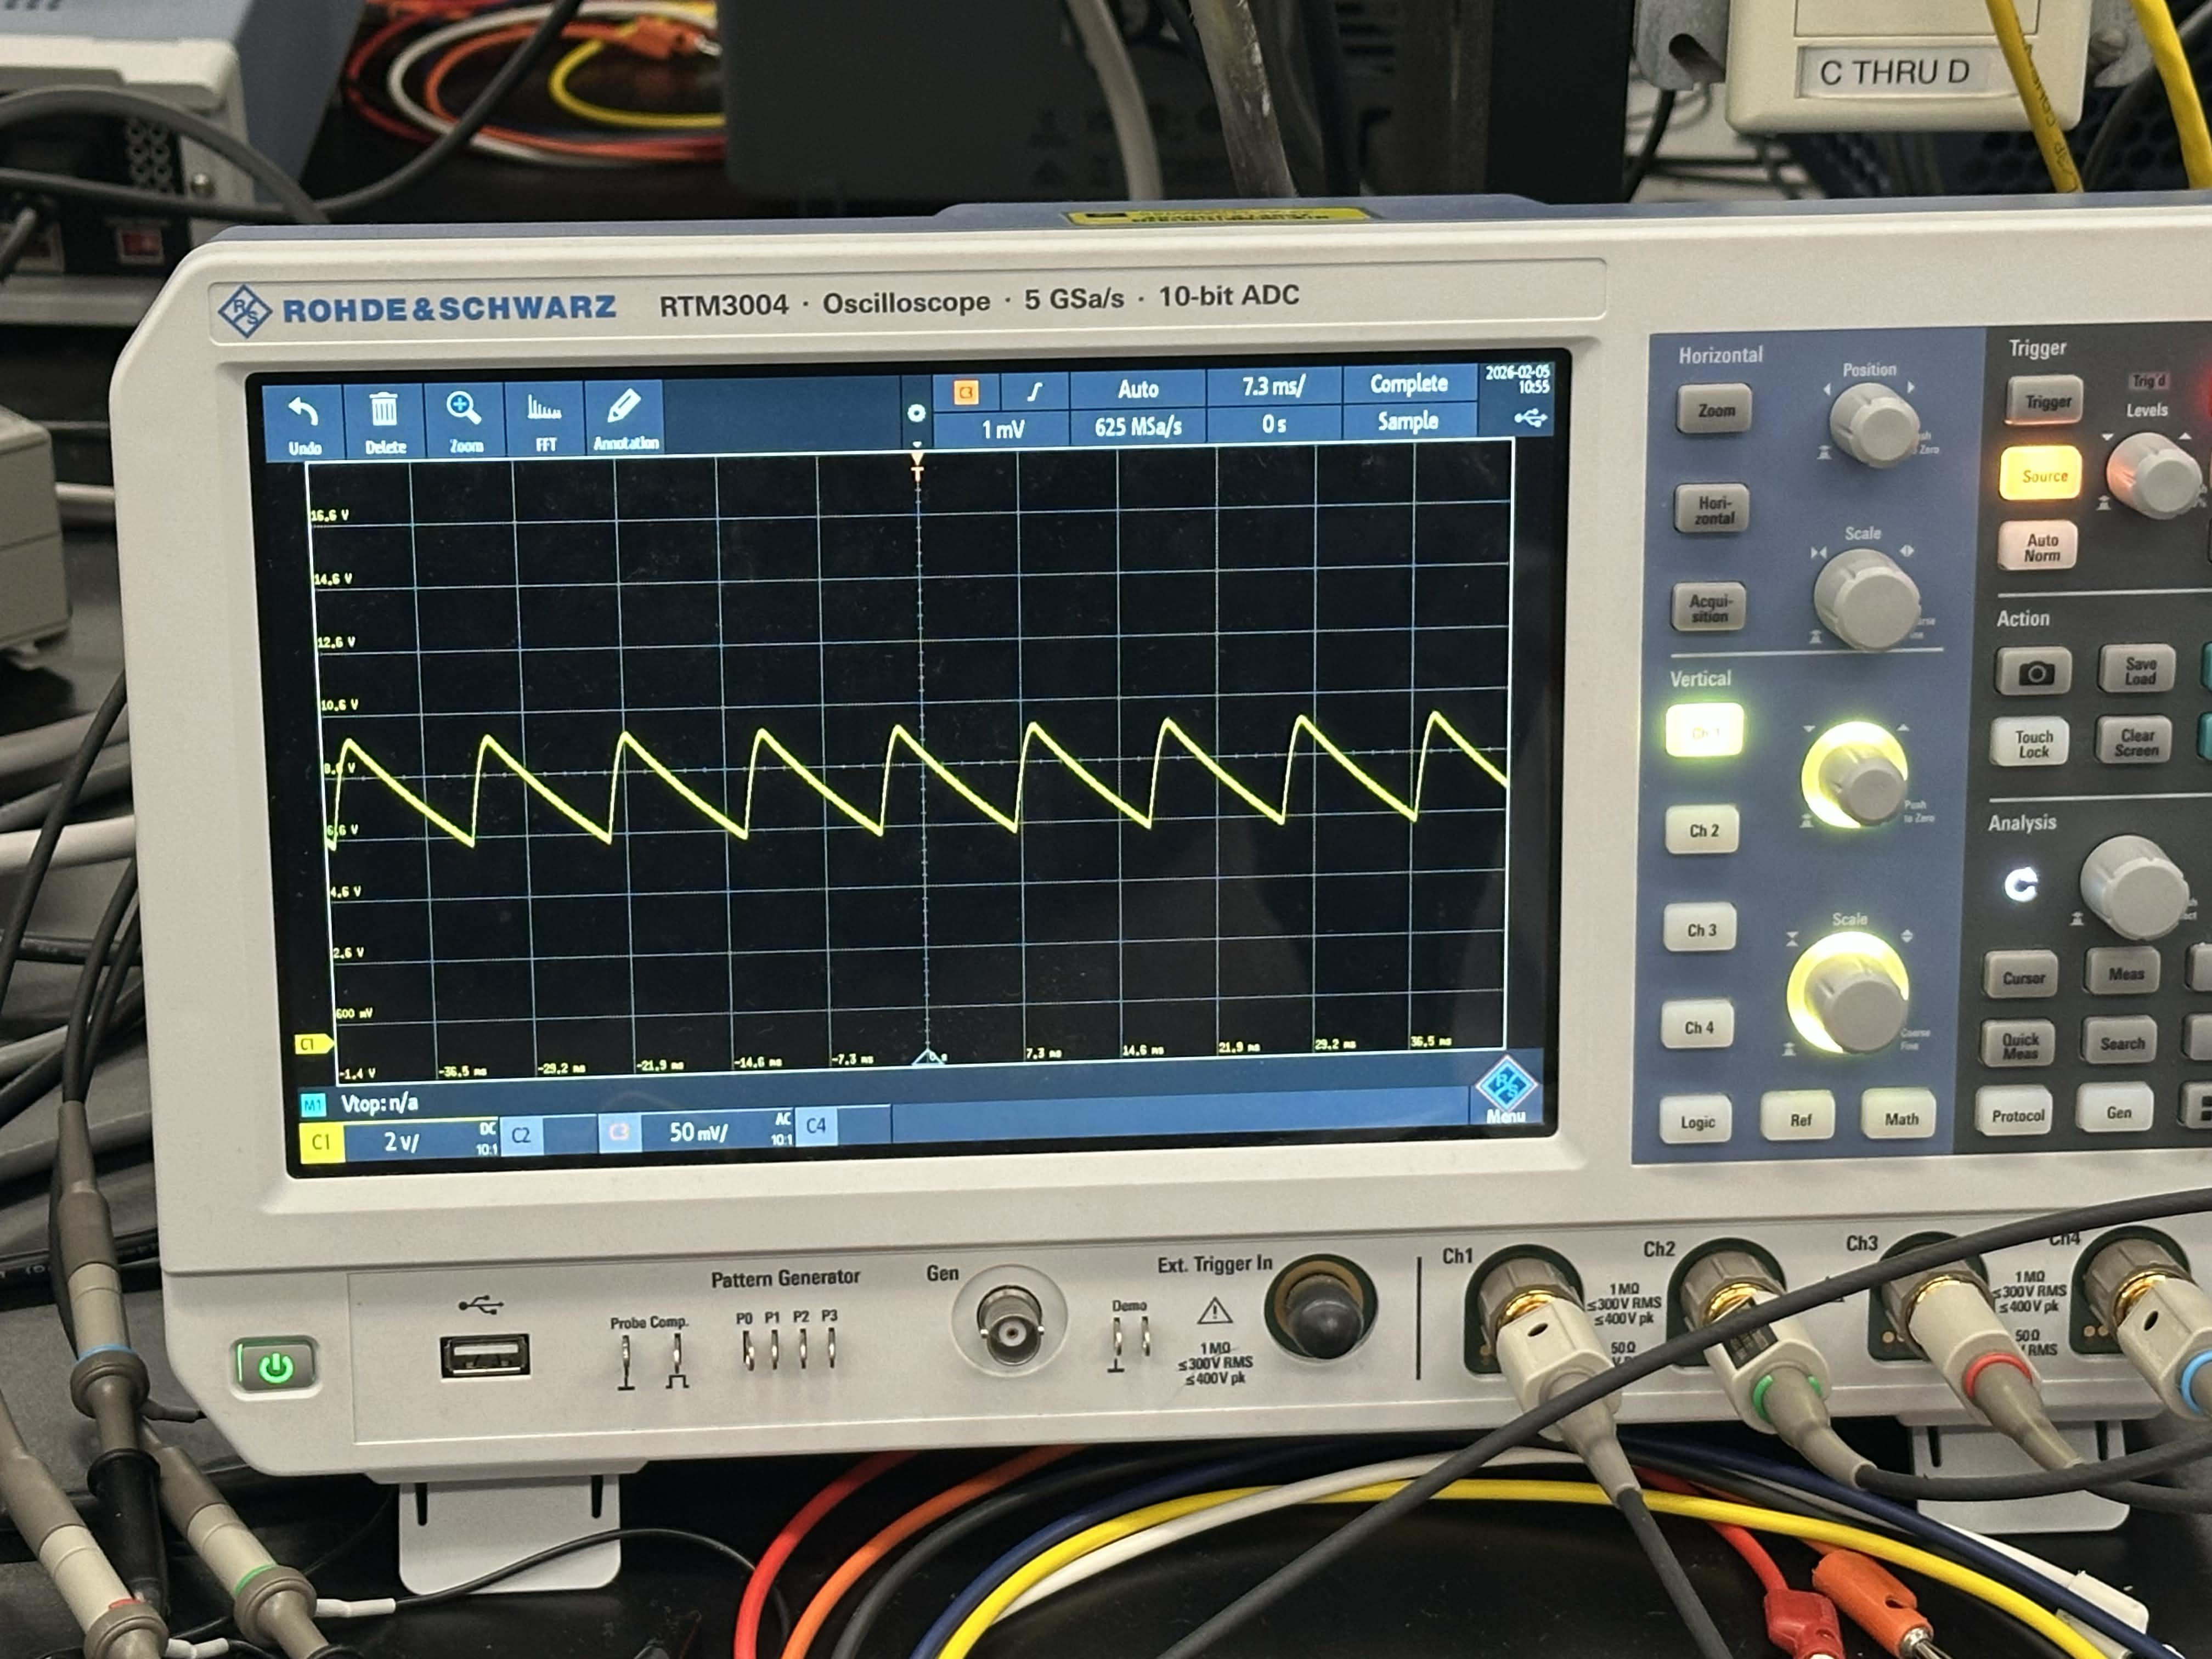
\includegraphics[width=\textwidth]{figure1_all_sine.jpg}
		\caption{Sinusoidal Input (Blue) vs Output (Yellow)}
		\label{fig:hw_all_sine}
	\end{subfigure}
	\hfill
	\begin{subfigure}[b]{0.48\textwidth}
		\centering
		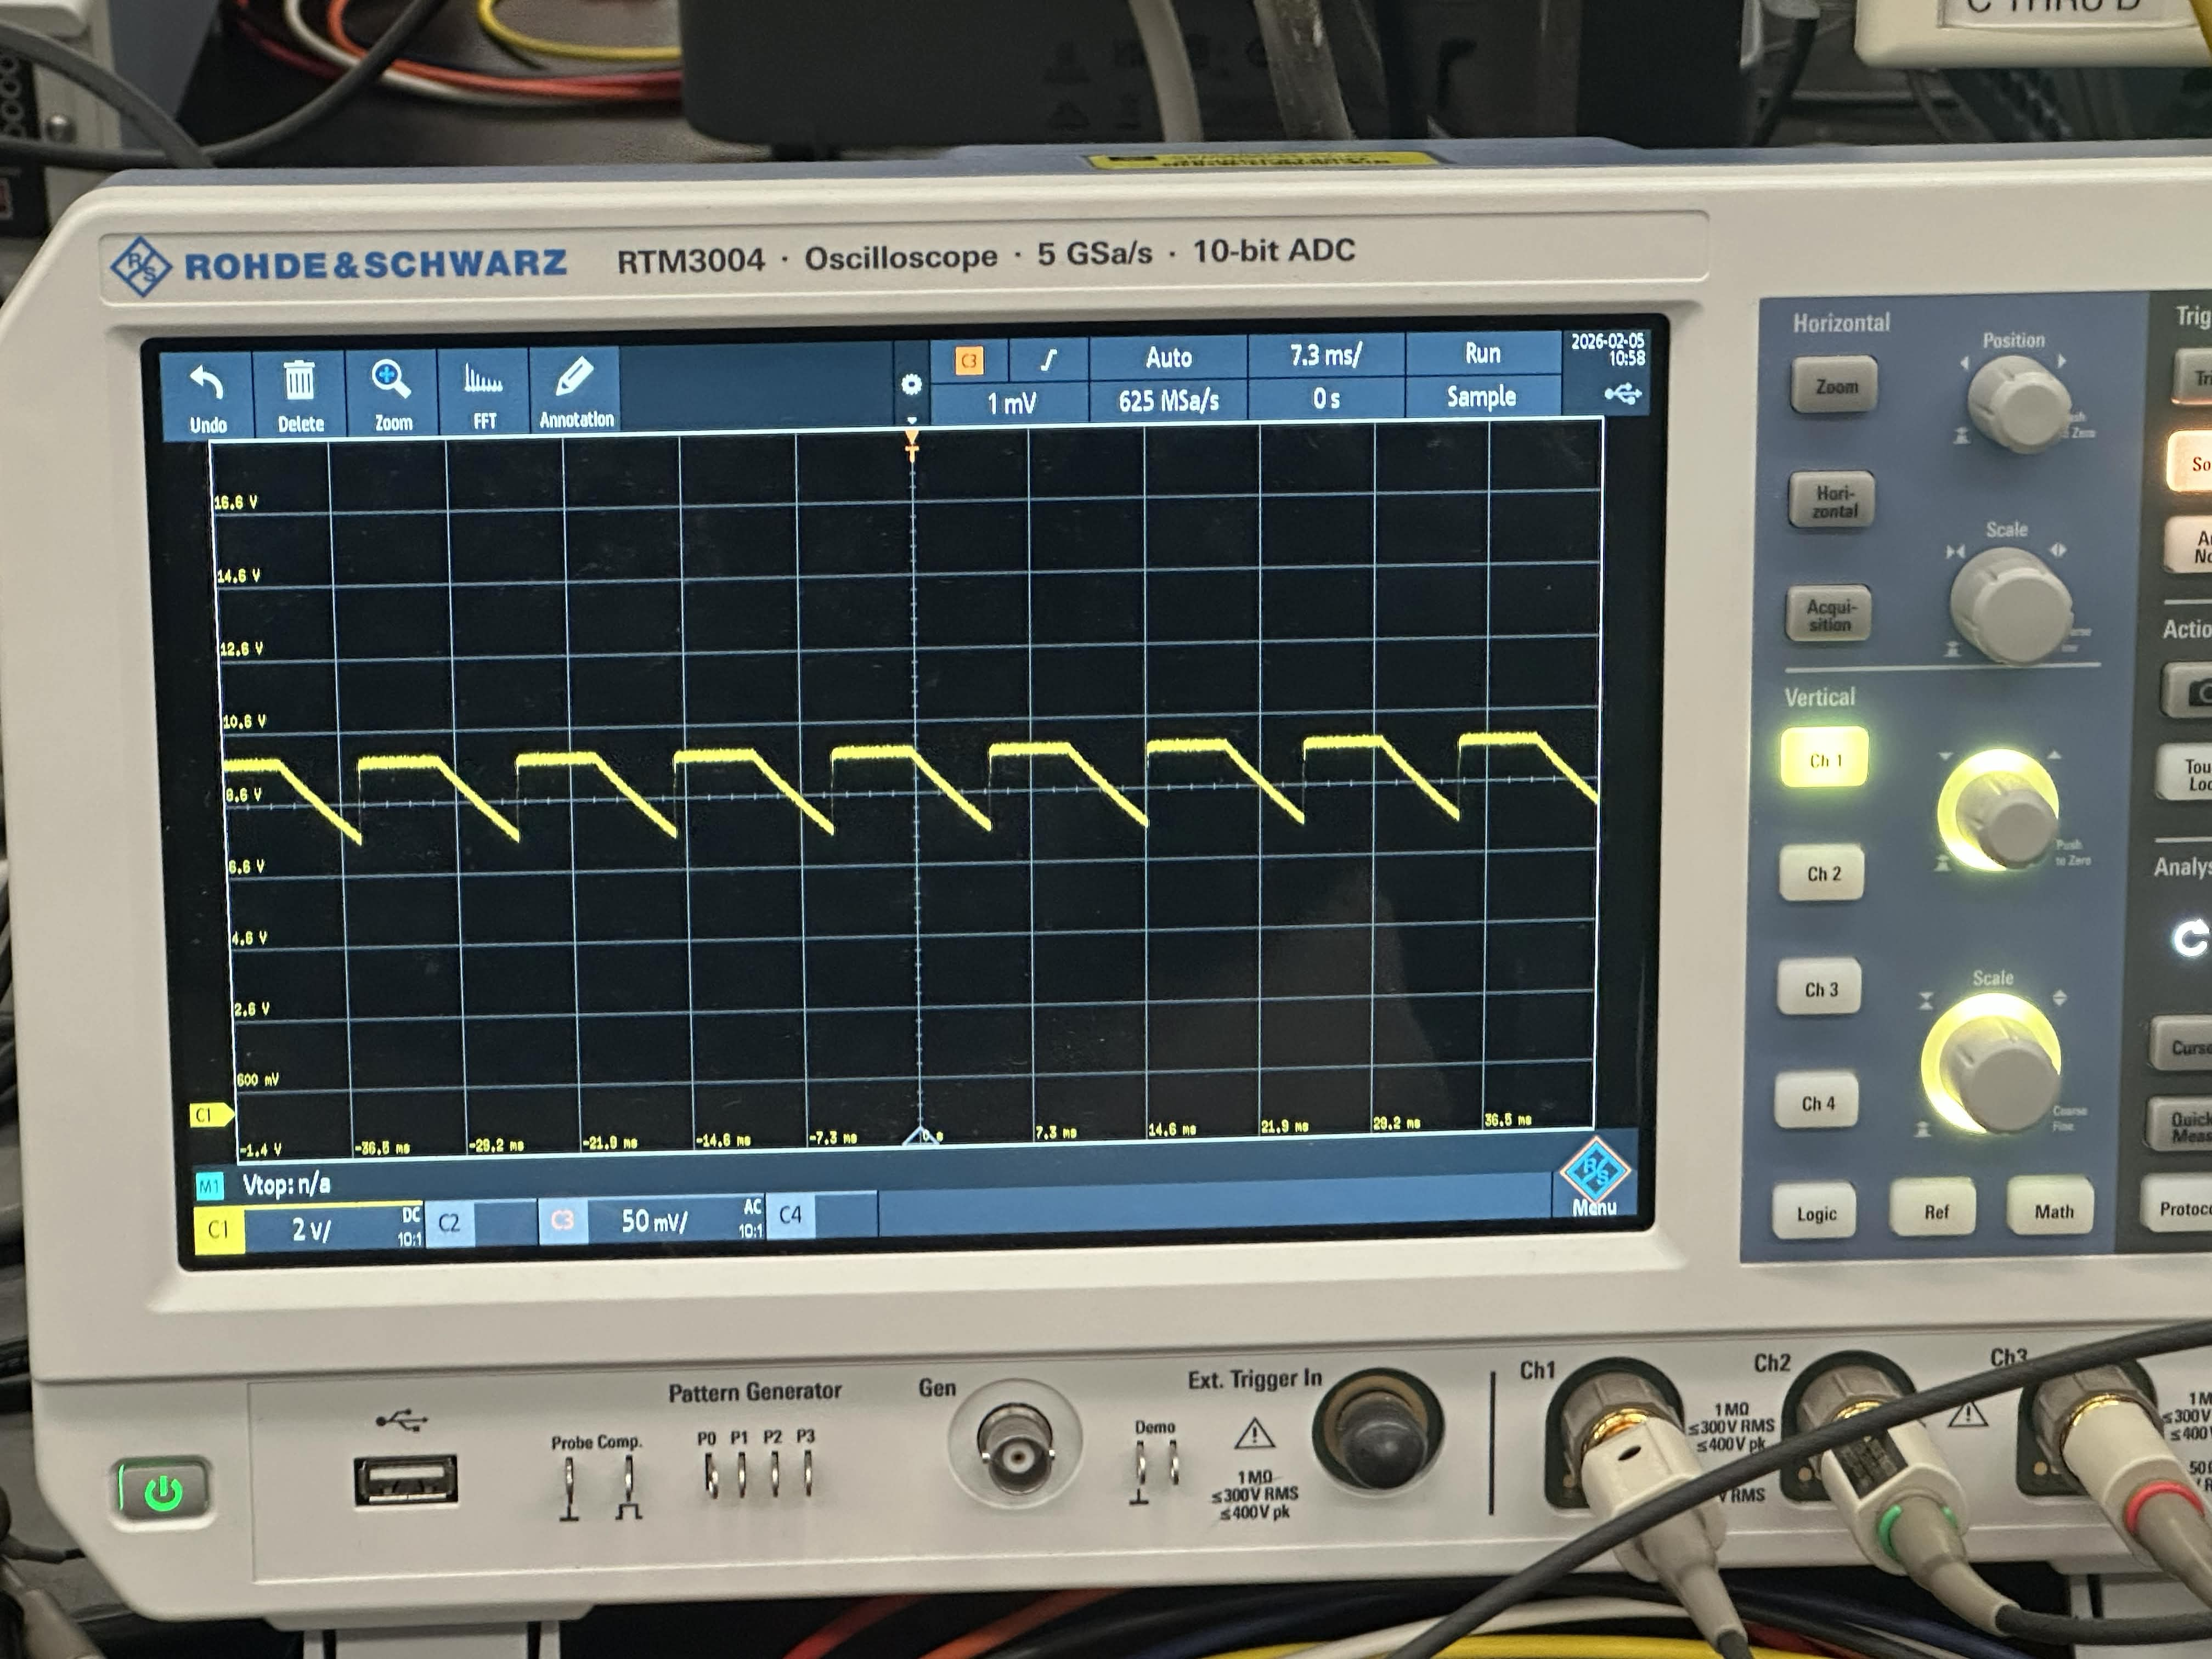
\includegraphics[width=\textwidth]{figure1_all_square.jpg}
		\caption{Square Input (Blue) vs Output (Yellow)}
		\label{fig:hw_all_square}
	\end{subfigure}
	\caption{Oscilloscope captures for the complete R-C-Diode half-wave peak rectifier.}
	\label{fig:hw_all_results}
\end{figure}

\begin{figure}[H]
	\centering
	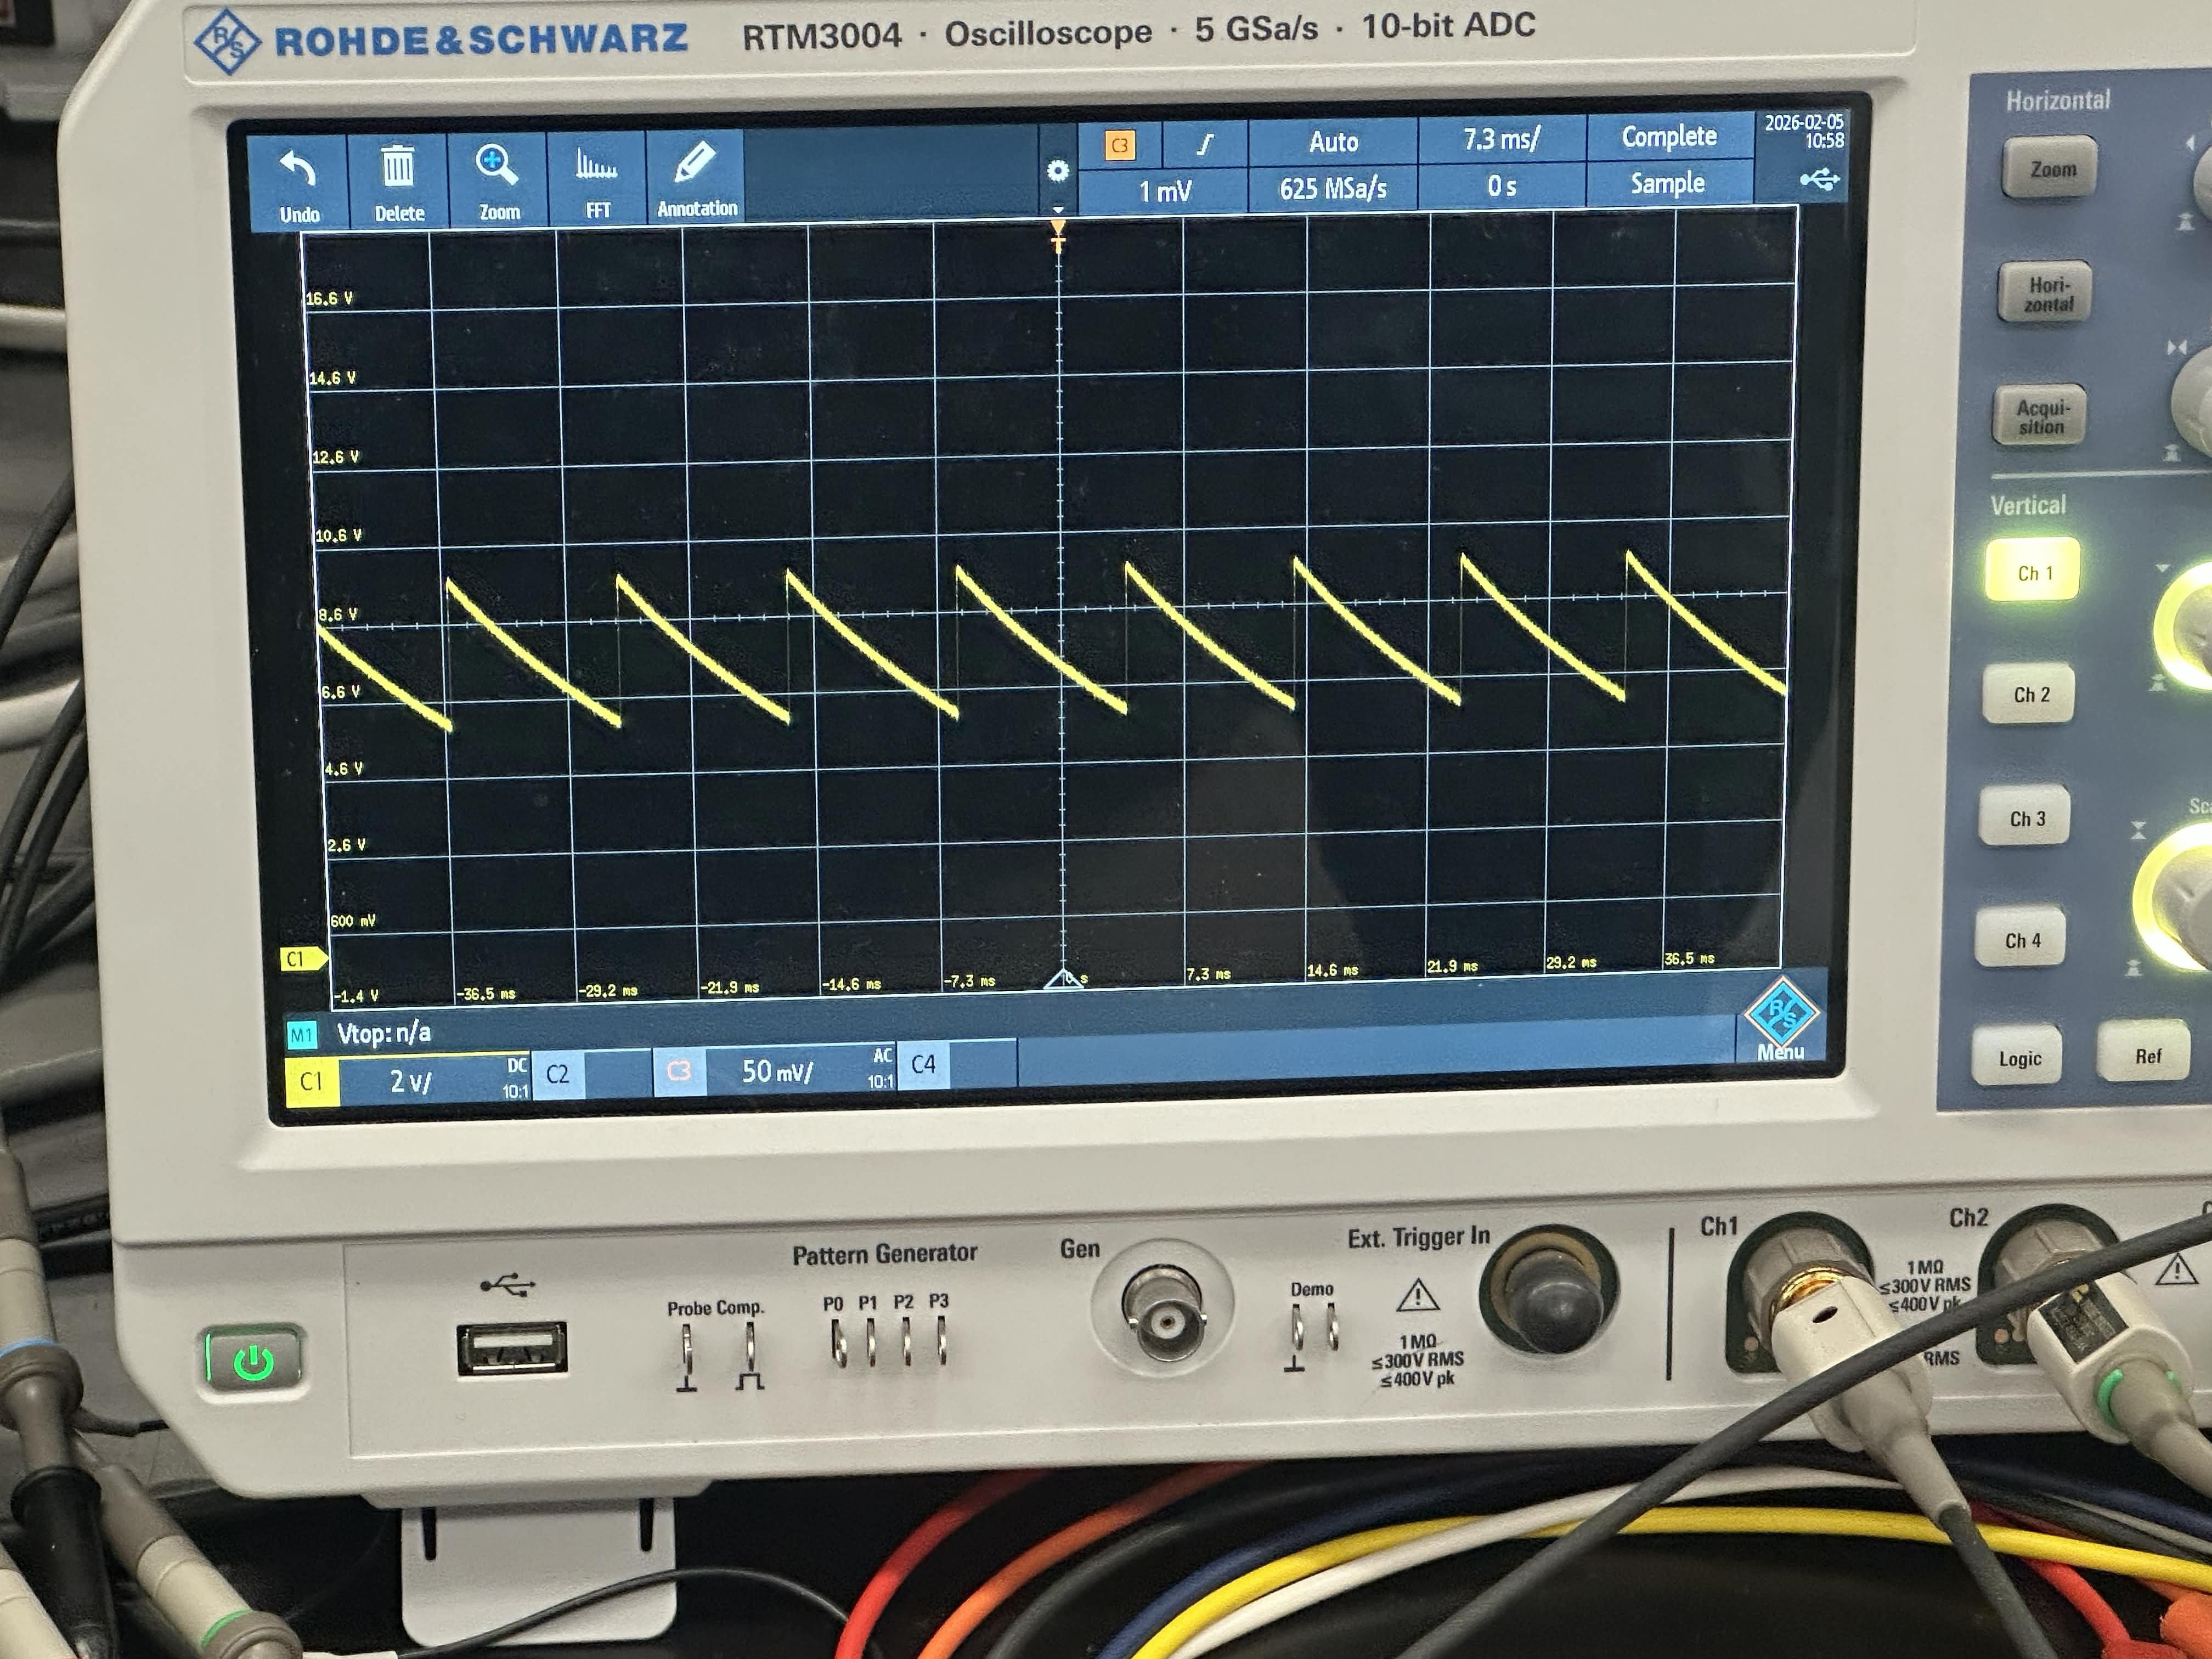
\includegraphics[width=0.6\textwidth]{figure1_all_triangle.jpg}
	\caption{Triangle wave response for the complete R-C-Diode half-wave peak rectifier.}
	\label{fig:hw_all_triangle}
\end{figure}

\textbf{Discussion:} \\
The waveforms in Figure~\ref{fig:hw_all_results} confirm the peak rectifier behavior:
\begin{itemize}
	\item \textbf{Charging Phase:} When the input voltage exceeds the capacitor voltage (plus the diode drop), the diode conducts, and the capacitor charges rapidly to the peak value of the input.
	\item \textbf{Discharging Phase:} When the input voltage falls below the peak, the diode becomes reverse-biased. The capacitor cannot discharge back through the diode; instead, it discharges slowly through the parallel load resistor ($R$).
	\item \textbf{Ripple Voltage:} This slow discharge creates a ``ripple'' on the DC output. The magnitude of this ripple is inversely proportional to the time constant $\tau = RC$. A larger time constant results in a smoother DC output voltage, closer to the ideal peak value.
	\item \textbf{Triangle Wave:} Figure~\ref{fig:hw_all_triangle} shows the circuit's response to a triangular wave input, demonstrating similar peak detection behavior.
\end{itemize}

\textbf{Calculation:}
With $R_L = 20\,\text{k}\Omega$ and $C = 10\,\mu\text{F}$, the time constant is:
\[
\tau = R_L C = (20 \times 10^3)(10 \times 10^{-6}) = 0.2\,\text{s}
\]
For a $100\,\text{Hz}$ input with $V_p = 5\,\text{V}$, the theoretical peak-to-peak ripple voltage is:
\[
V_{r(pp)} = \frac{V_p - V_{on}}{f \cdot R_L \cdot C} = \frac{5.0 - 0.7}{100 \times 0.2} = \frac{4.3}{20} = 0.215\,\text{V}
\]
This small ripple ($\approx 5\%$ of $V_p$) is consistent with the near-DC output observed in the oscilloscope captures, confirming effective filtering by the $RC$ network.

%-----------------------------------------
% FULL-WAVE RECTIFIER (Lab Manual Fig. 2)
%-----------------------------------------
\subsection{Full-Wave Rectifier (Lab Manual Fig.~2)}
The full-wave rectifier uses a center-tapped transformer or two-diode bridge to rectify both halves of the input cycle, reducing the ripple by a factor of two compared to the half-wave rectifier.

\subsubsection{Part A: No Capacitor}
\begin{figure}[H]
	\centering
	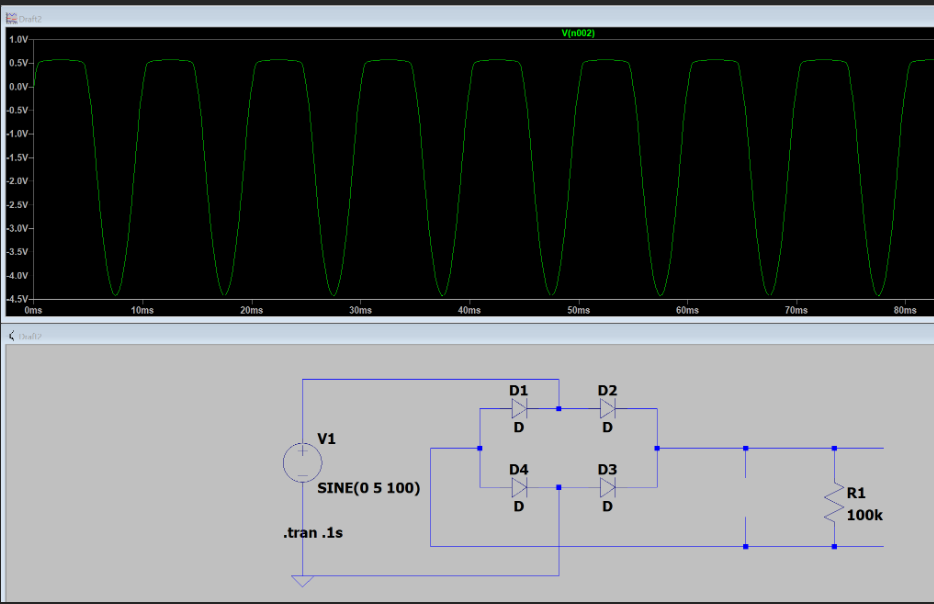
\includegraphics[width=0.6\textwidth]{figure2_nocapacitor_ltspice.png}
	\caption{LTspice simulation schematic for the full-wave rectifier without capacitor.}
	\label{fig:fw_sch_nocap}
\end{figure}

\begin{figure}[H]
	\centering
	\begin{subfigure}[b]{0.48\textwidth}
		\centering
		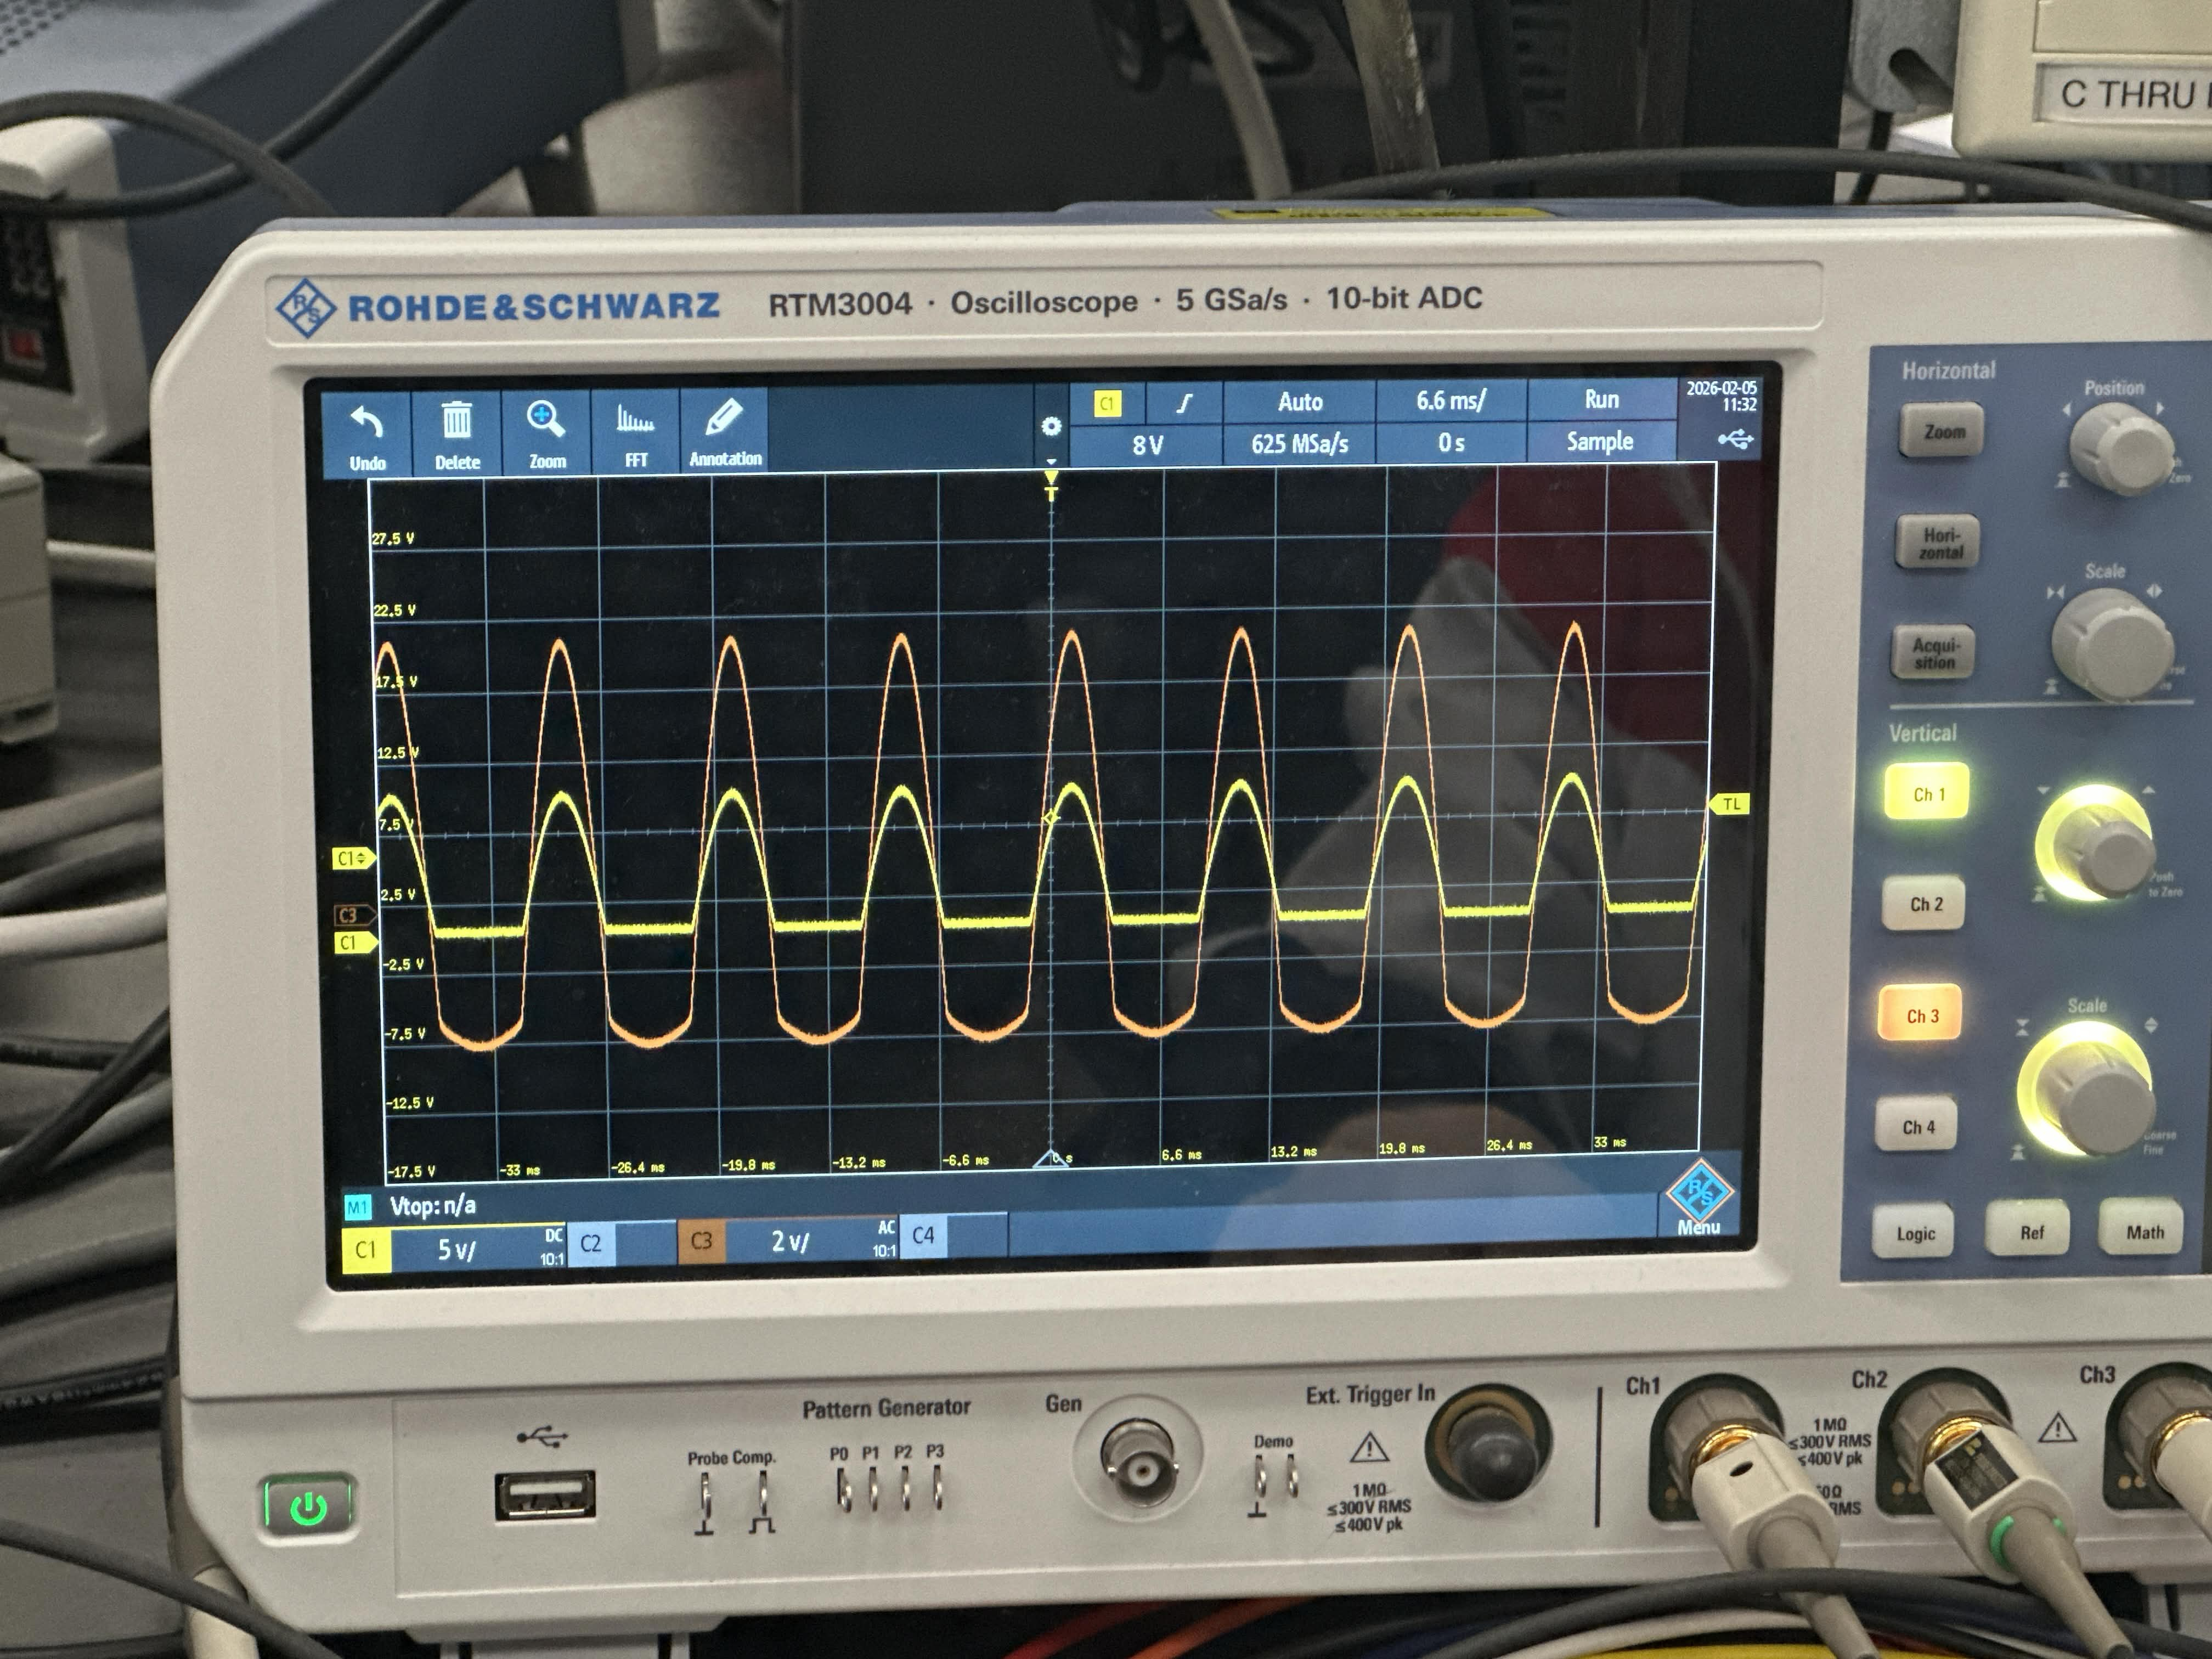
\includegraphics[width=\textwidth]{figure2_nocapacitor_sine.jpg}
		\caption{Sinusoidal Input (Blue) vs Output (Yellow)}
		\label{fig:fw_nocap_sine}
	\end{subfigure}
	\hfill
	\begin{subfigure}[b]{0.48\textwidth}
		\centering
		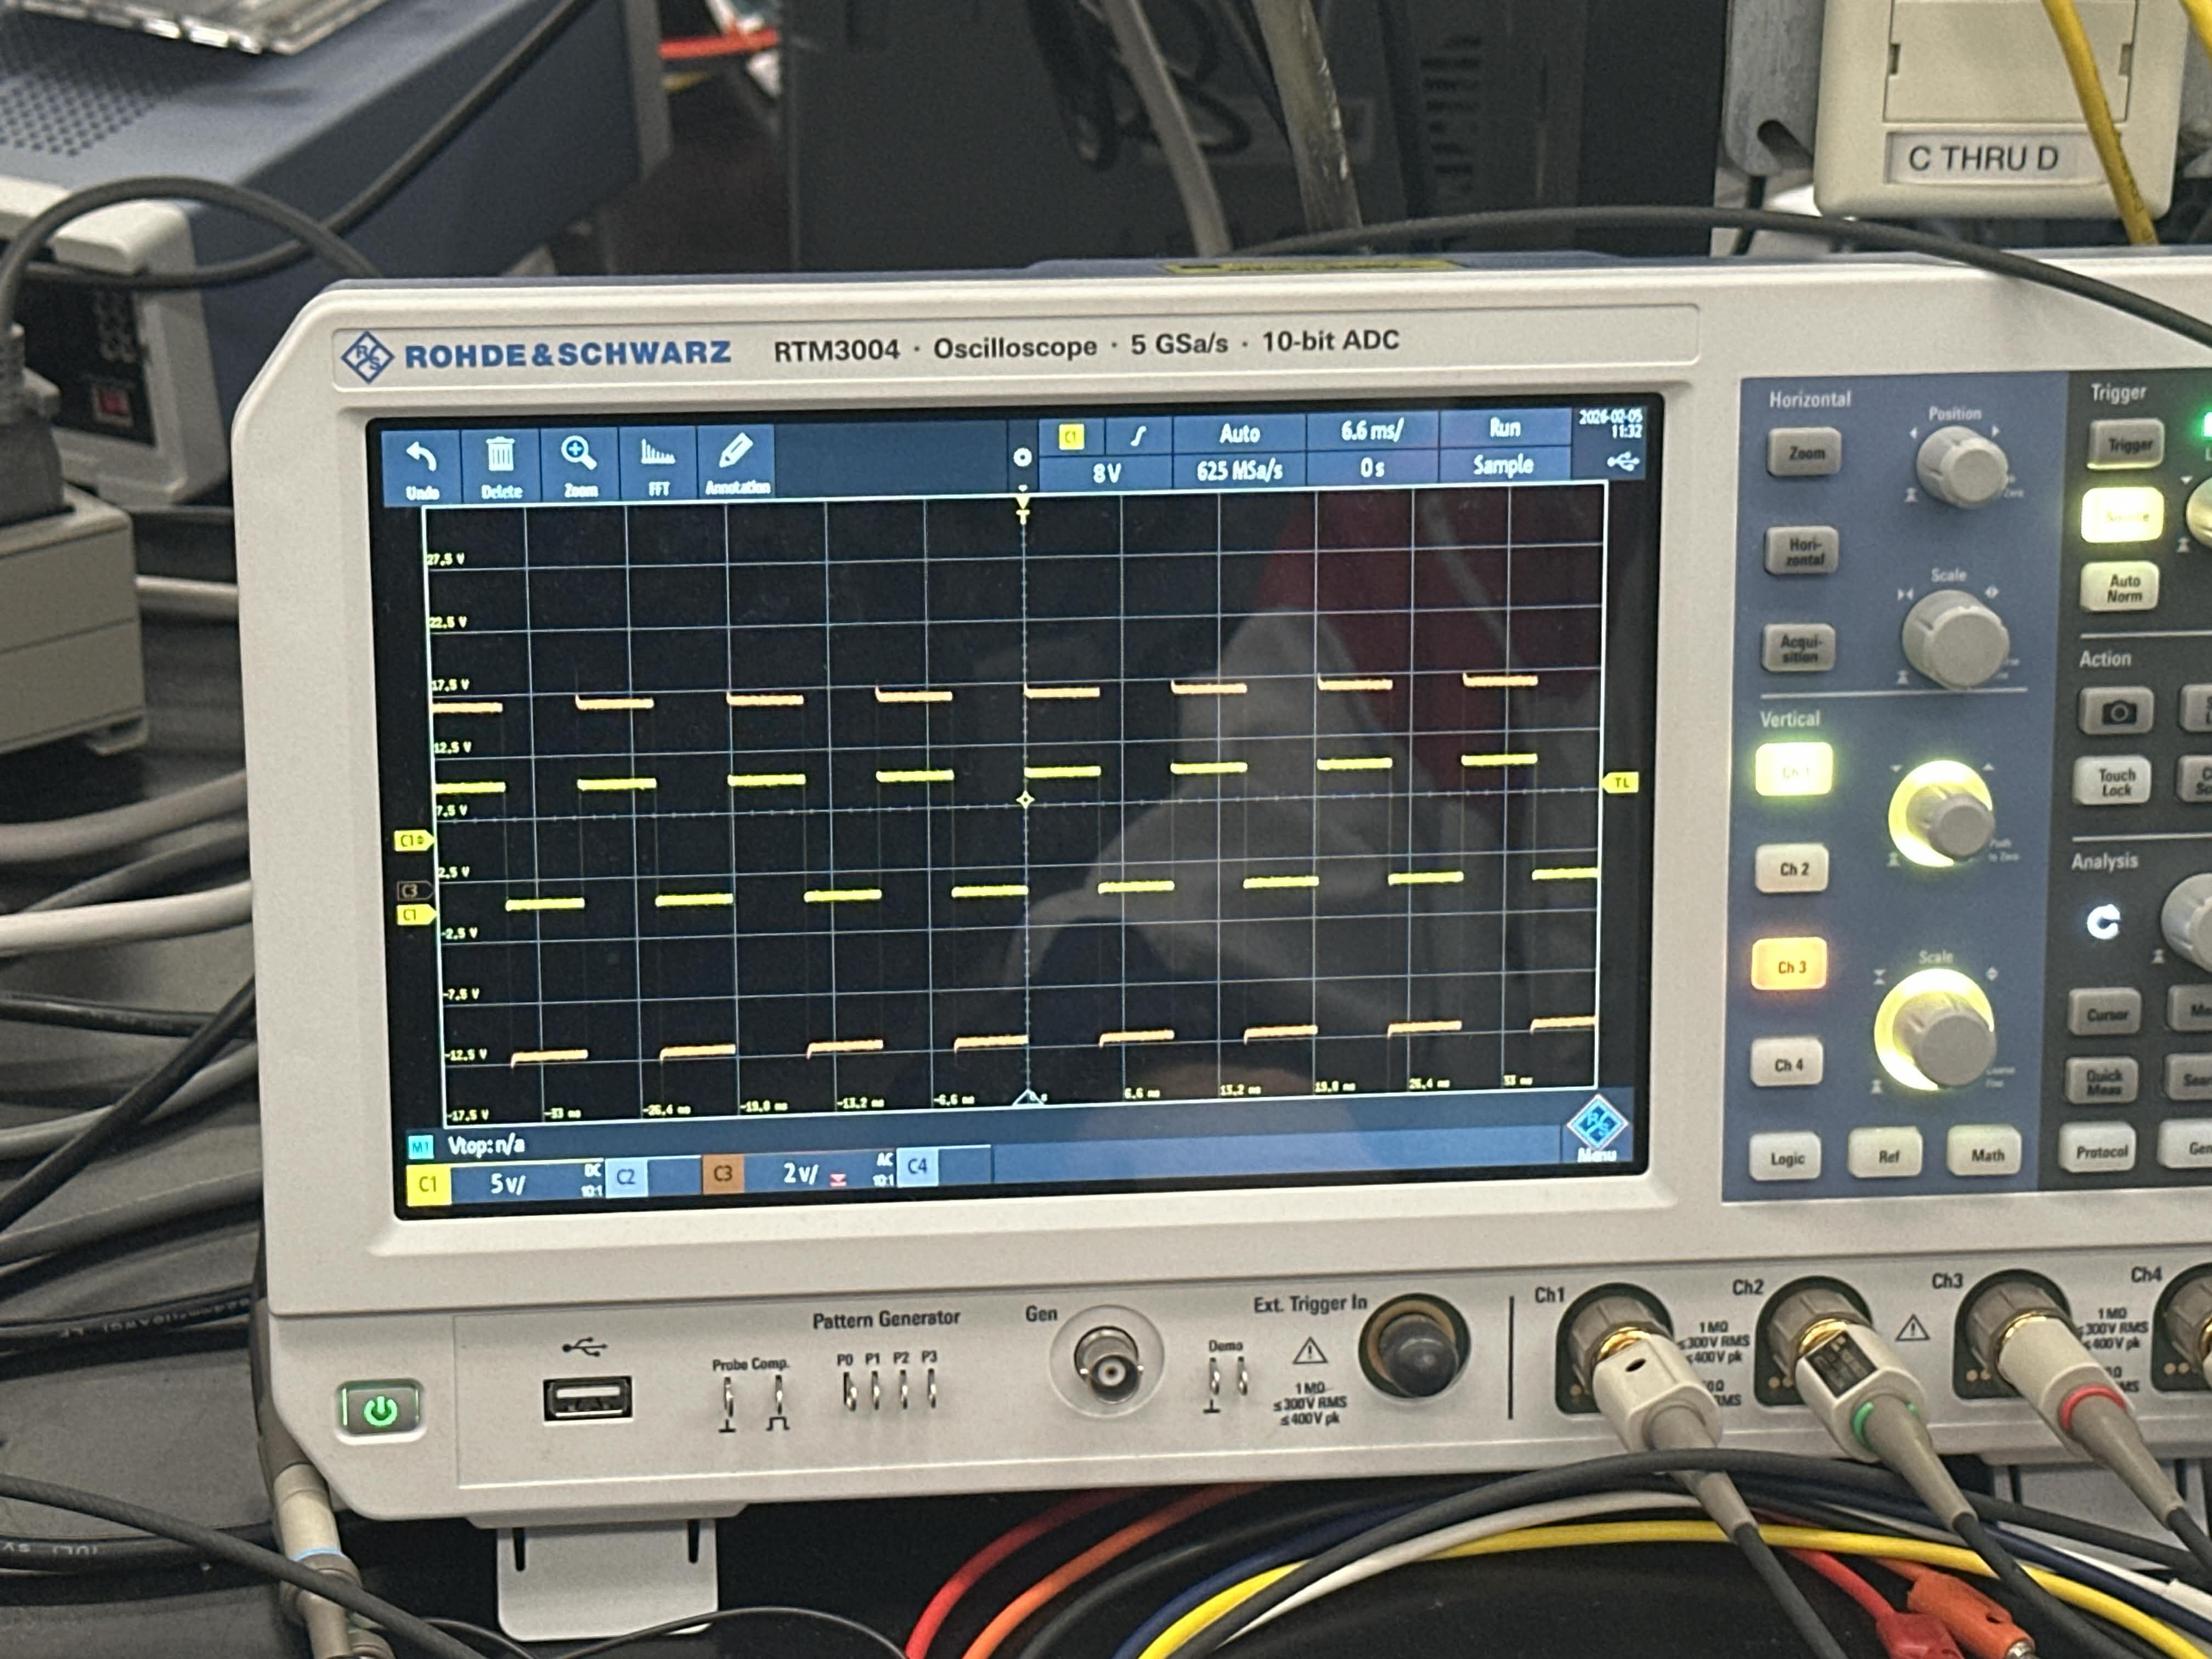
\includegraphics[width=\textwidth]{figure2_nocapacitor_square.jpg}
		\caption{Square Input (Blue) vs Output (Yellow)}
		\label{fig:fw_nocap_square}
	\end{subfigure}
	\caption{Oscilloscope captures for the full-wave rectifier without capacitor.}
	\label{fig:fw_nocap_results}
\end{figure}

\textbf{Discussion:} \\
The full-wave rectifier without a capacitor inverts the negative half-cycles, producing a pulsating DC output at twice the input frequency. Both halves of the input cycle contribute to the output, improving energy efficiency over the half-wave rectifier. The diode voltage drop ($\approx 0.7\,\text{V}$) is visible on each half-cycle.

\textbf{Calculation:}
The transfer characteristic for the full-wave rectifier is:
\[
V_{out} = |V_{in}| - V_{on} \quad \text{for } |V_{in}| > V_{on}, \qquad V_{out} = 0 \quad \text{otherwise}
\]
The peak output voltage is identical to the half-wave case ($V_{out,peak} = 4.3\,\text{V}$), but the output frequency is $2f = 200\,\text{Hz}$, as both positive and negative input half-cycles contribute to the output.

\subsubsection{Part B: No Resistor}
The experimental oscilloscope captures for the full-wave circuit with the resistor removed are presented in Figure~\ref{fig:fw_nores_results}.

\begin{figure}[H]
	\centering
	\begin{subfigure}[b]{0.48\textwidth}
		\centering
		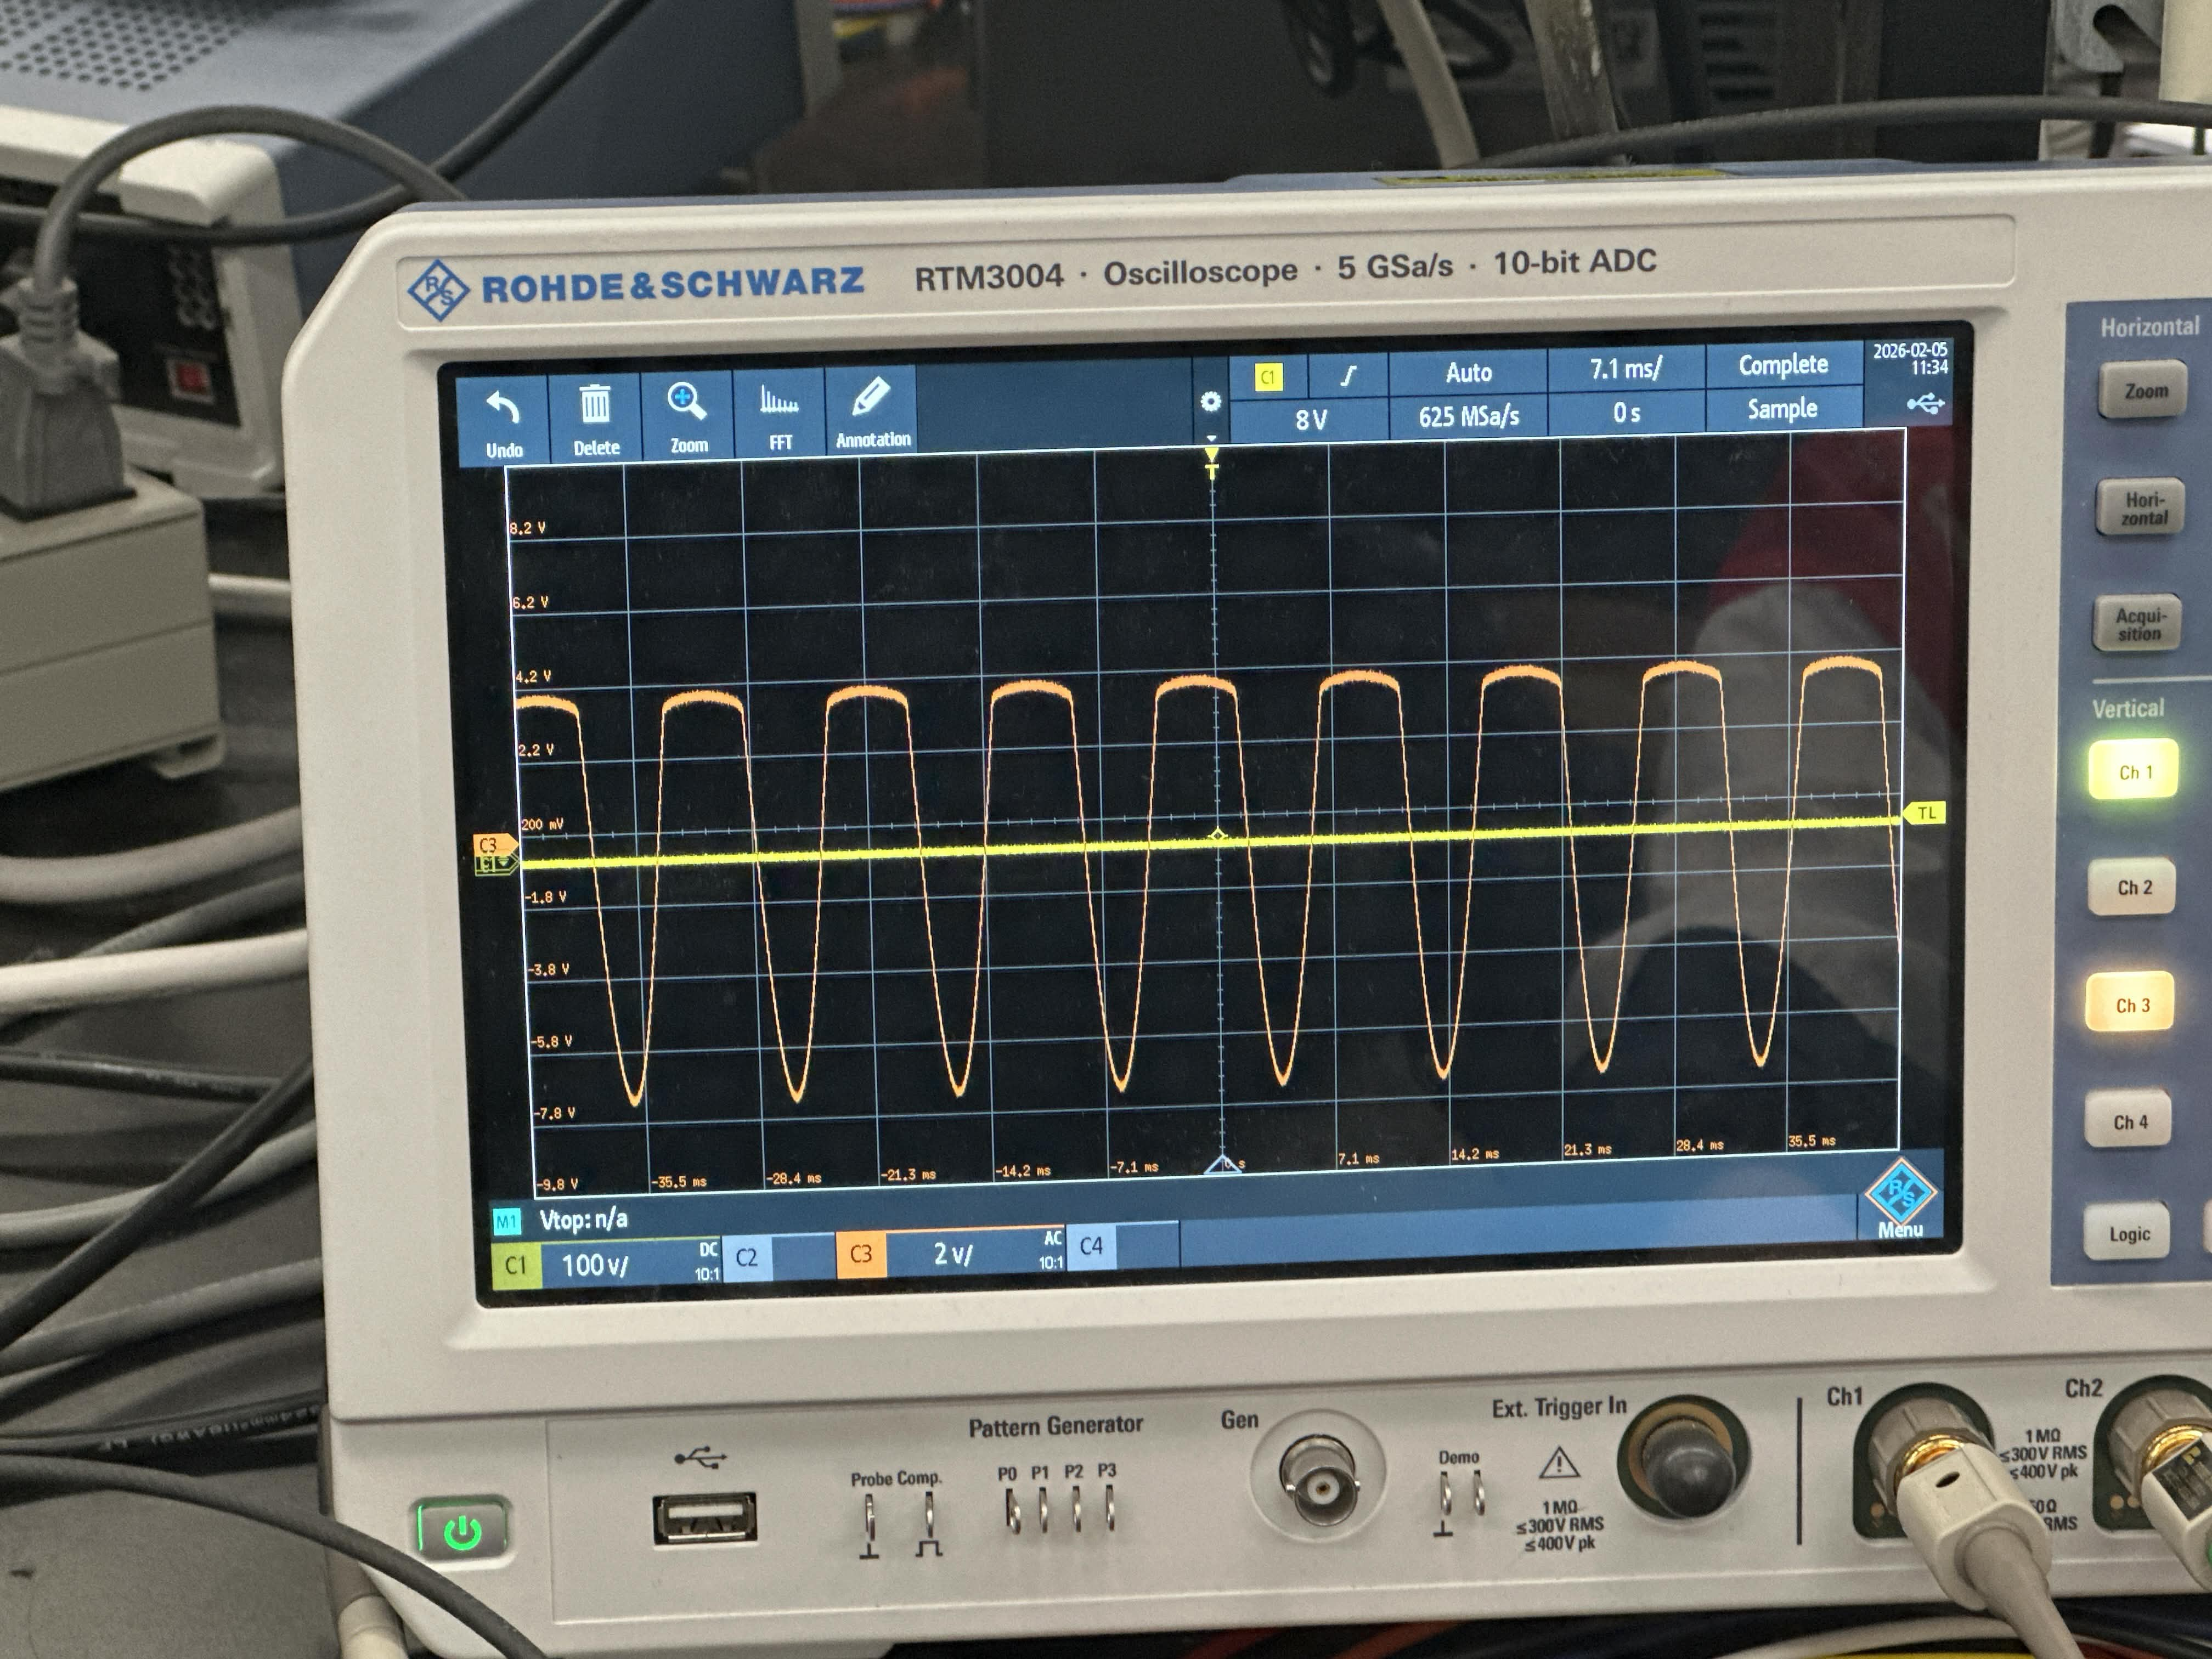
\includegraphics[width=\textwidth]{figure2_noresistor_sine.jpg}
		\caption{Sinusoidal Input (Blue) vs Output (Yellow)}
		\label{fig:fw_nores_sine}
	\end{subfigure}
	\hfill
	\begin{subfigure}[b]{0.48\textwidth}
		\centering
		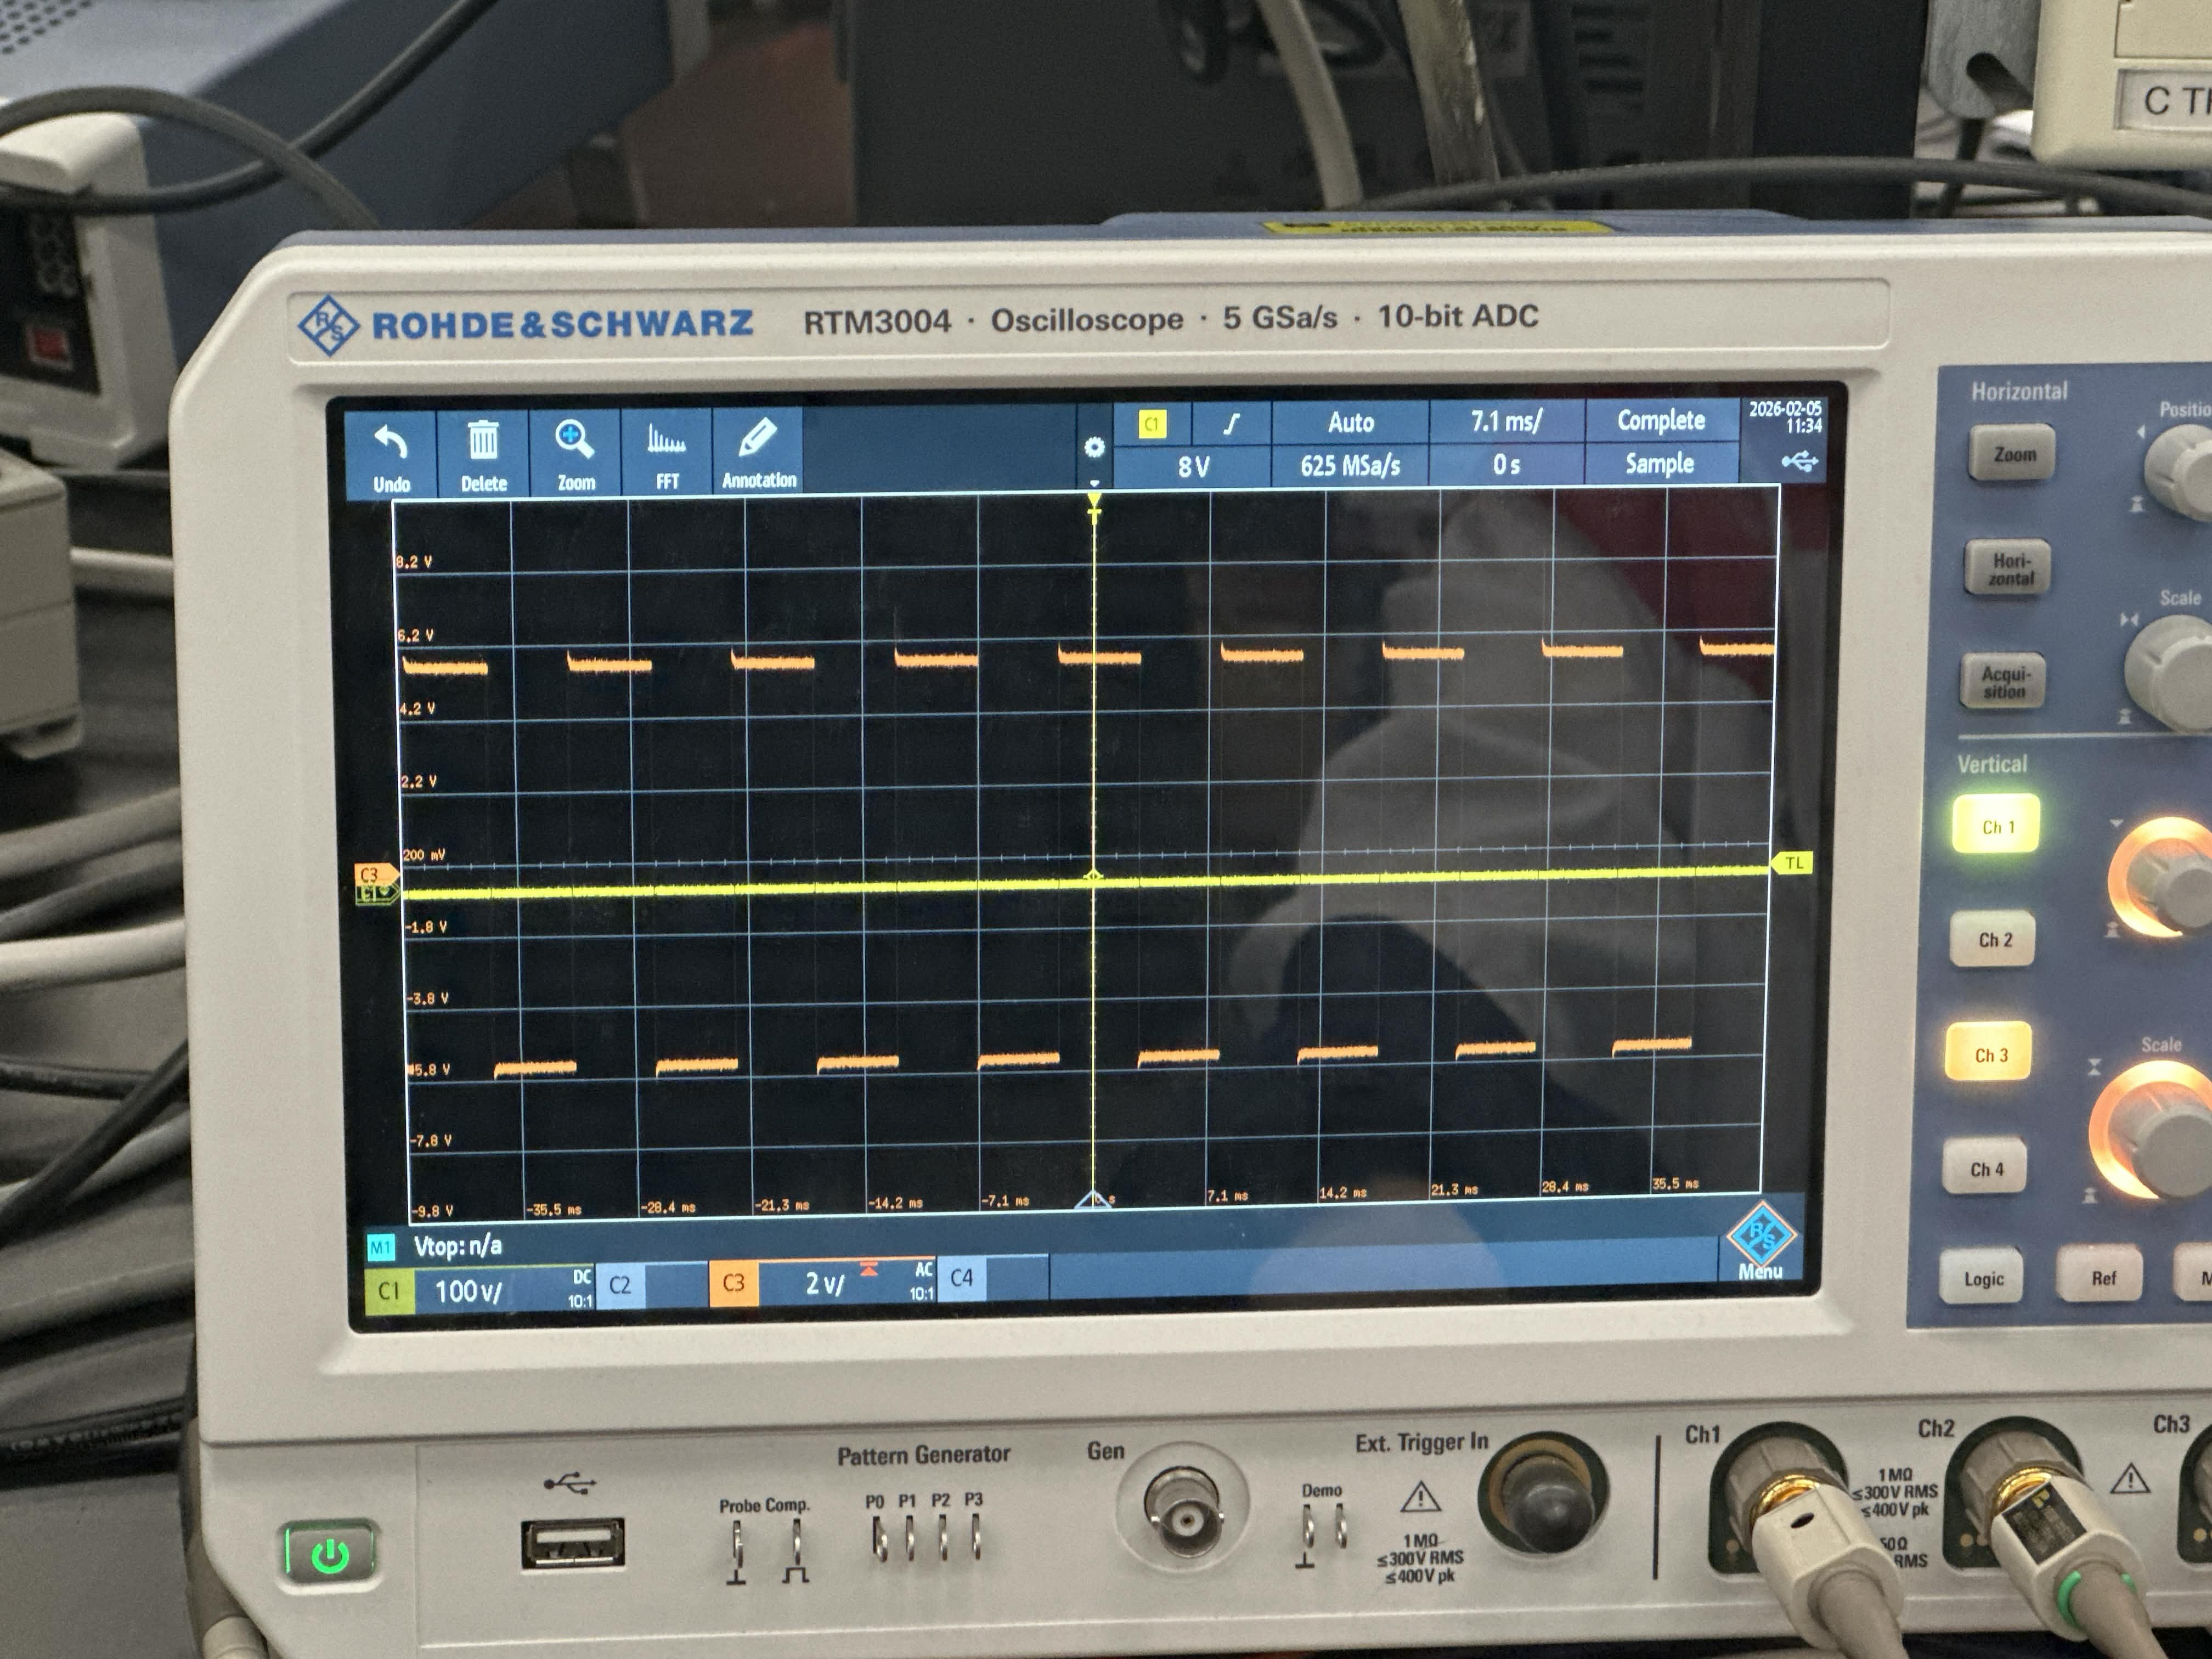
\includegraphics[width=\textwidth]{figure2_noresistor_square.jpg}
		\caption{Square Input (Blue) vs Output (Yellow)}
		\label{fig:fw_nores_square}
	\end{subfigure}
	\caption{Oscilloscope captures for the full-wave circuit without resistor.}
	\label{fig:fw_nores_results}
\end{figure}

\textbf{Discussion:} \\
With the resistor removed, the capacitor and diode form a full-wave clamping configuration. The capacitor charges during each half-cycle through the forward-biased diode and holds its charge when the diode is reverse-biased, resulting in a DC level shift of the full-wave rectified signal.

\subsubsection{Part C: Complete Circuit}
\begin{figure}[H]
	\centering
	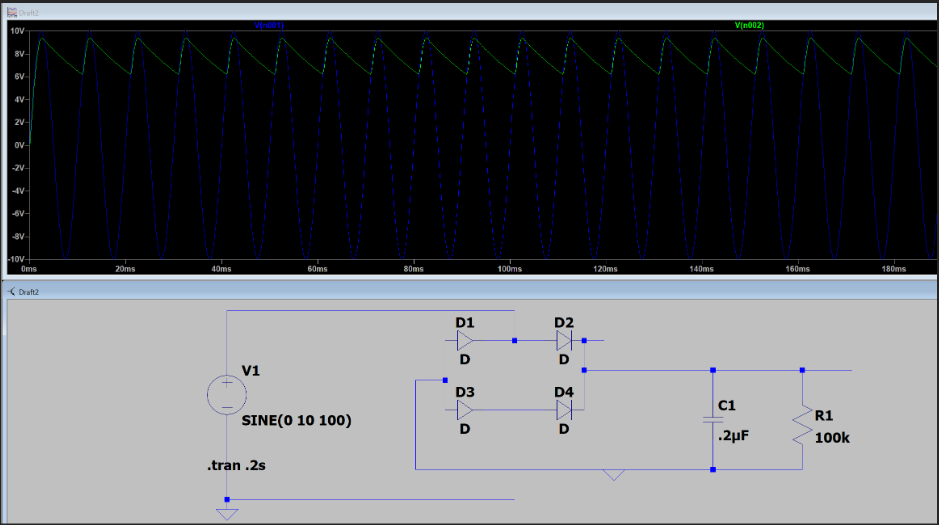
\includegraphics[width=0.6\textwidth]{figure2_all_ltspice.png}
	\caption{LTspice simulation schematic for the complete full-wave R-C-Diode circuit.}
	\label{fig:fw_sch_all}
\end{figure}

\begin{figure}[H]
	\centering
	\begin{subfigure}[b]{0.48\textwidth}
		\centering
		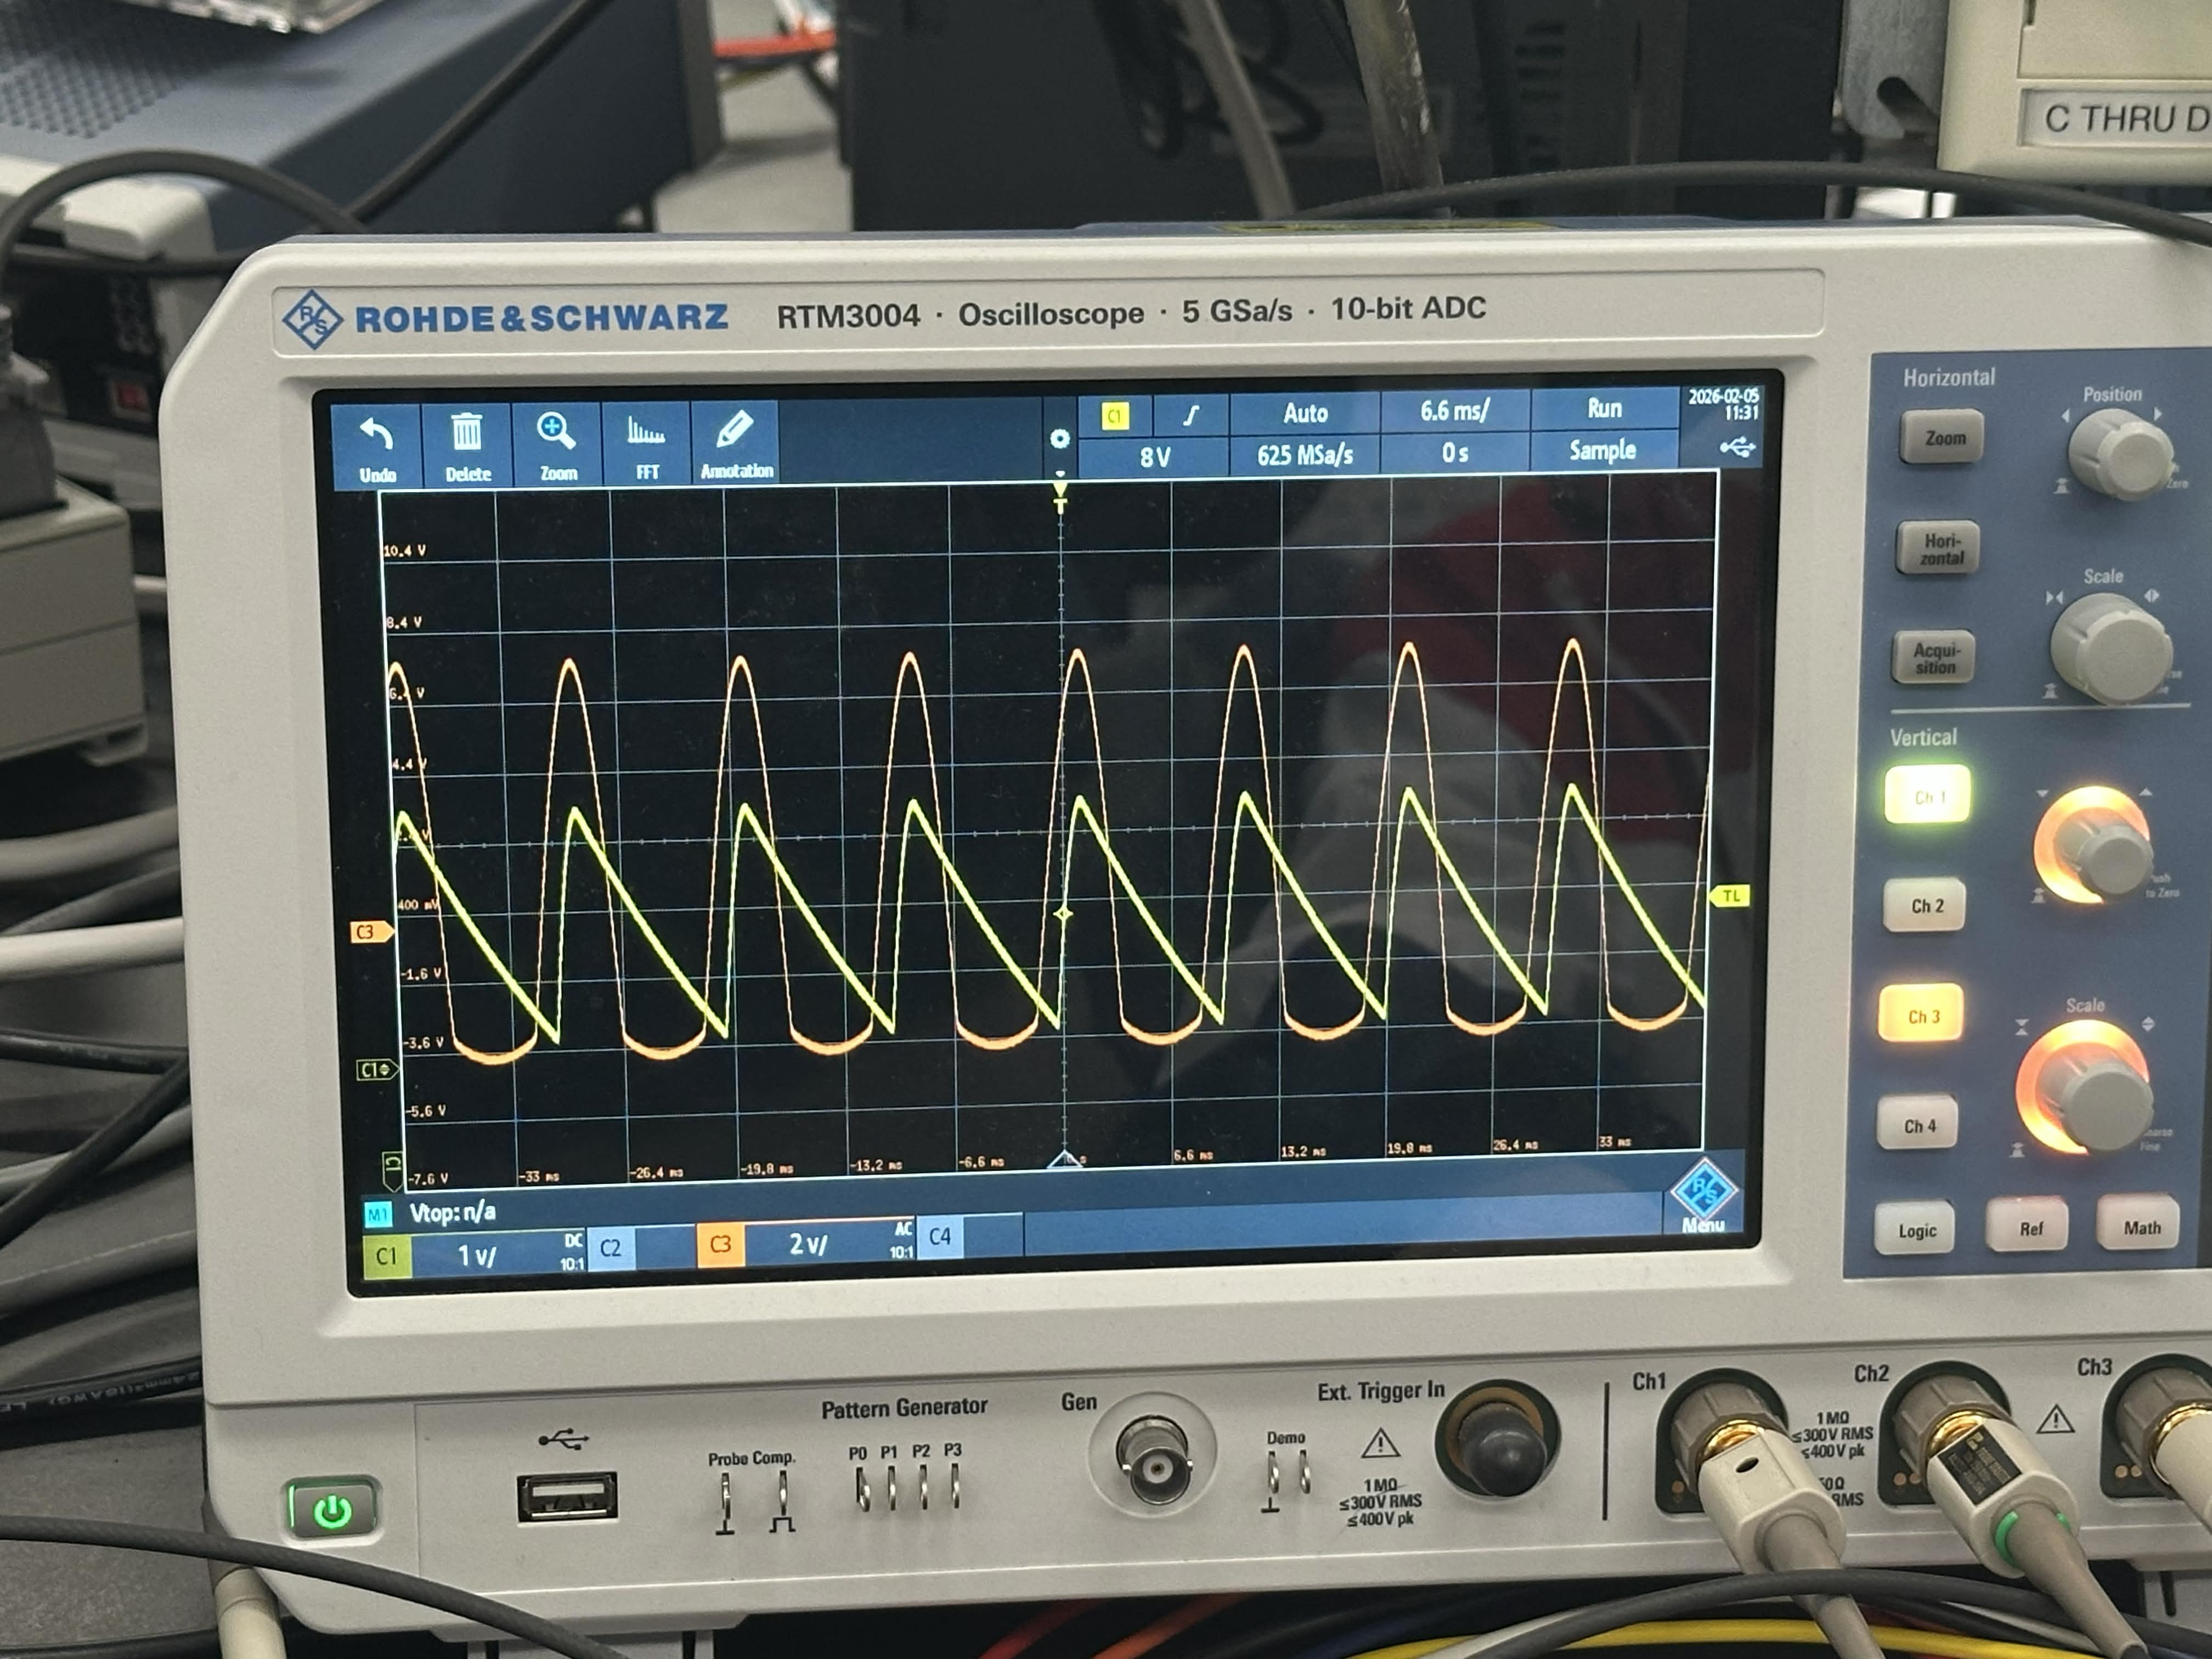
\includegraphics[width=\textwidth]{figure2_all_sine.jpg}
		\caption{Sinusoidal Input (Blue) vs Output (Yellow)}
		\label{fig:fw_all_sine}
	\end{subfigure}
	\hfill
	\begin{subfigure}[b]{0.48\textwidth}
		\centering
		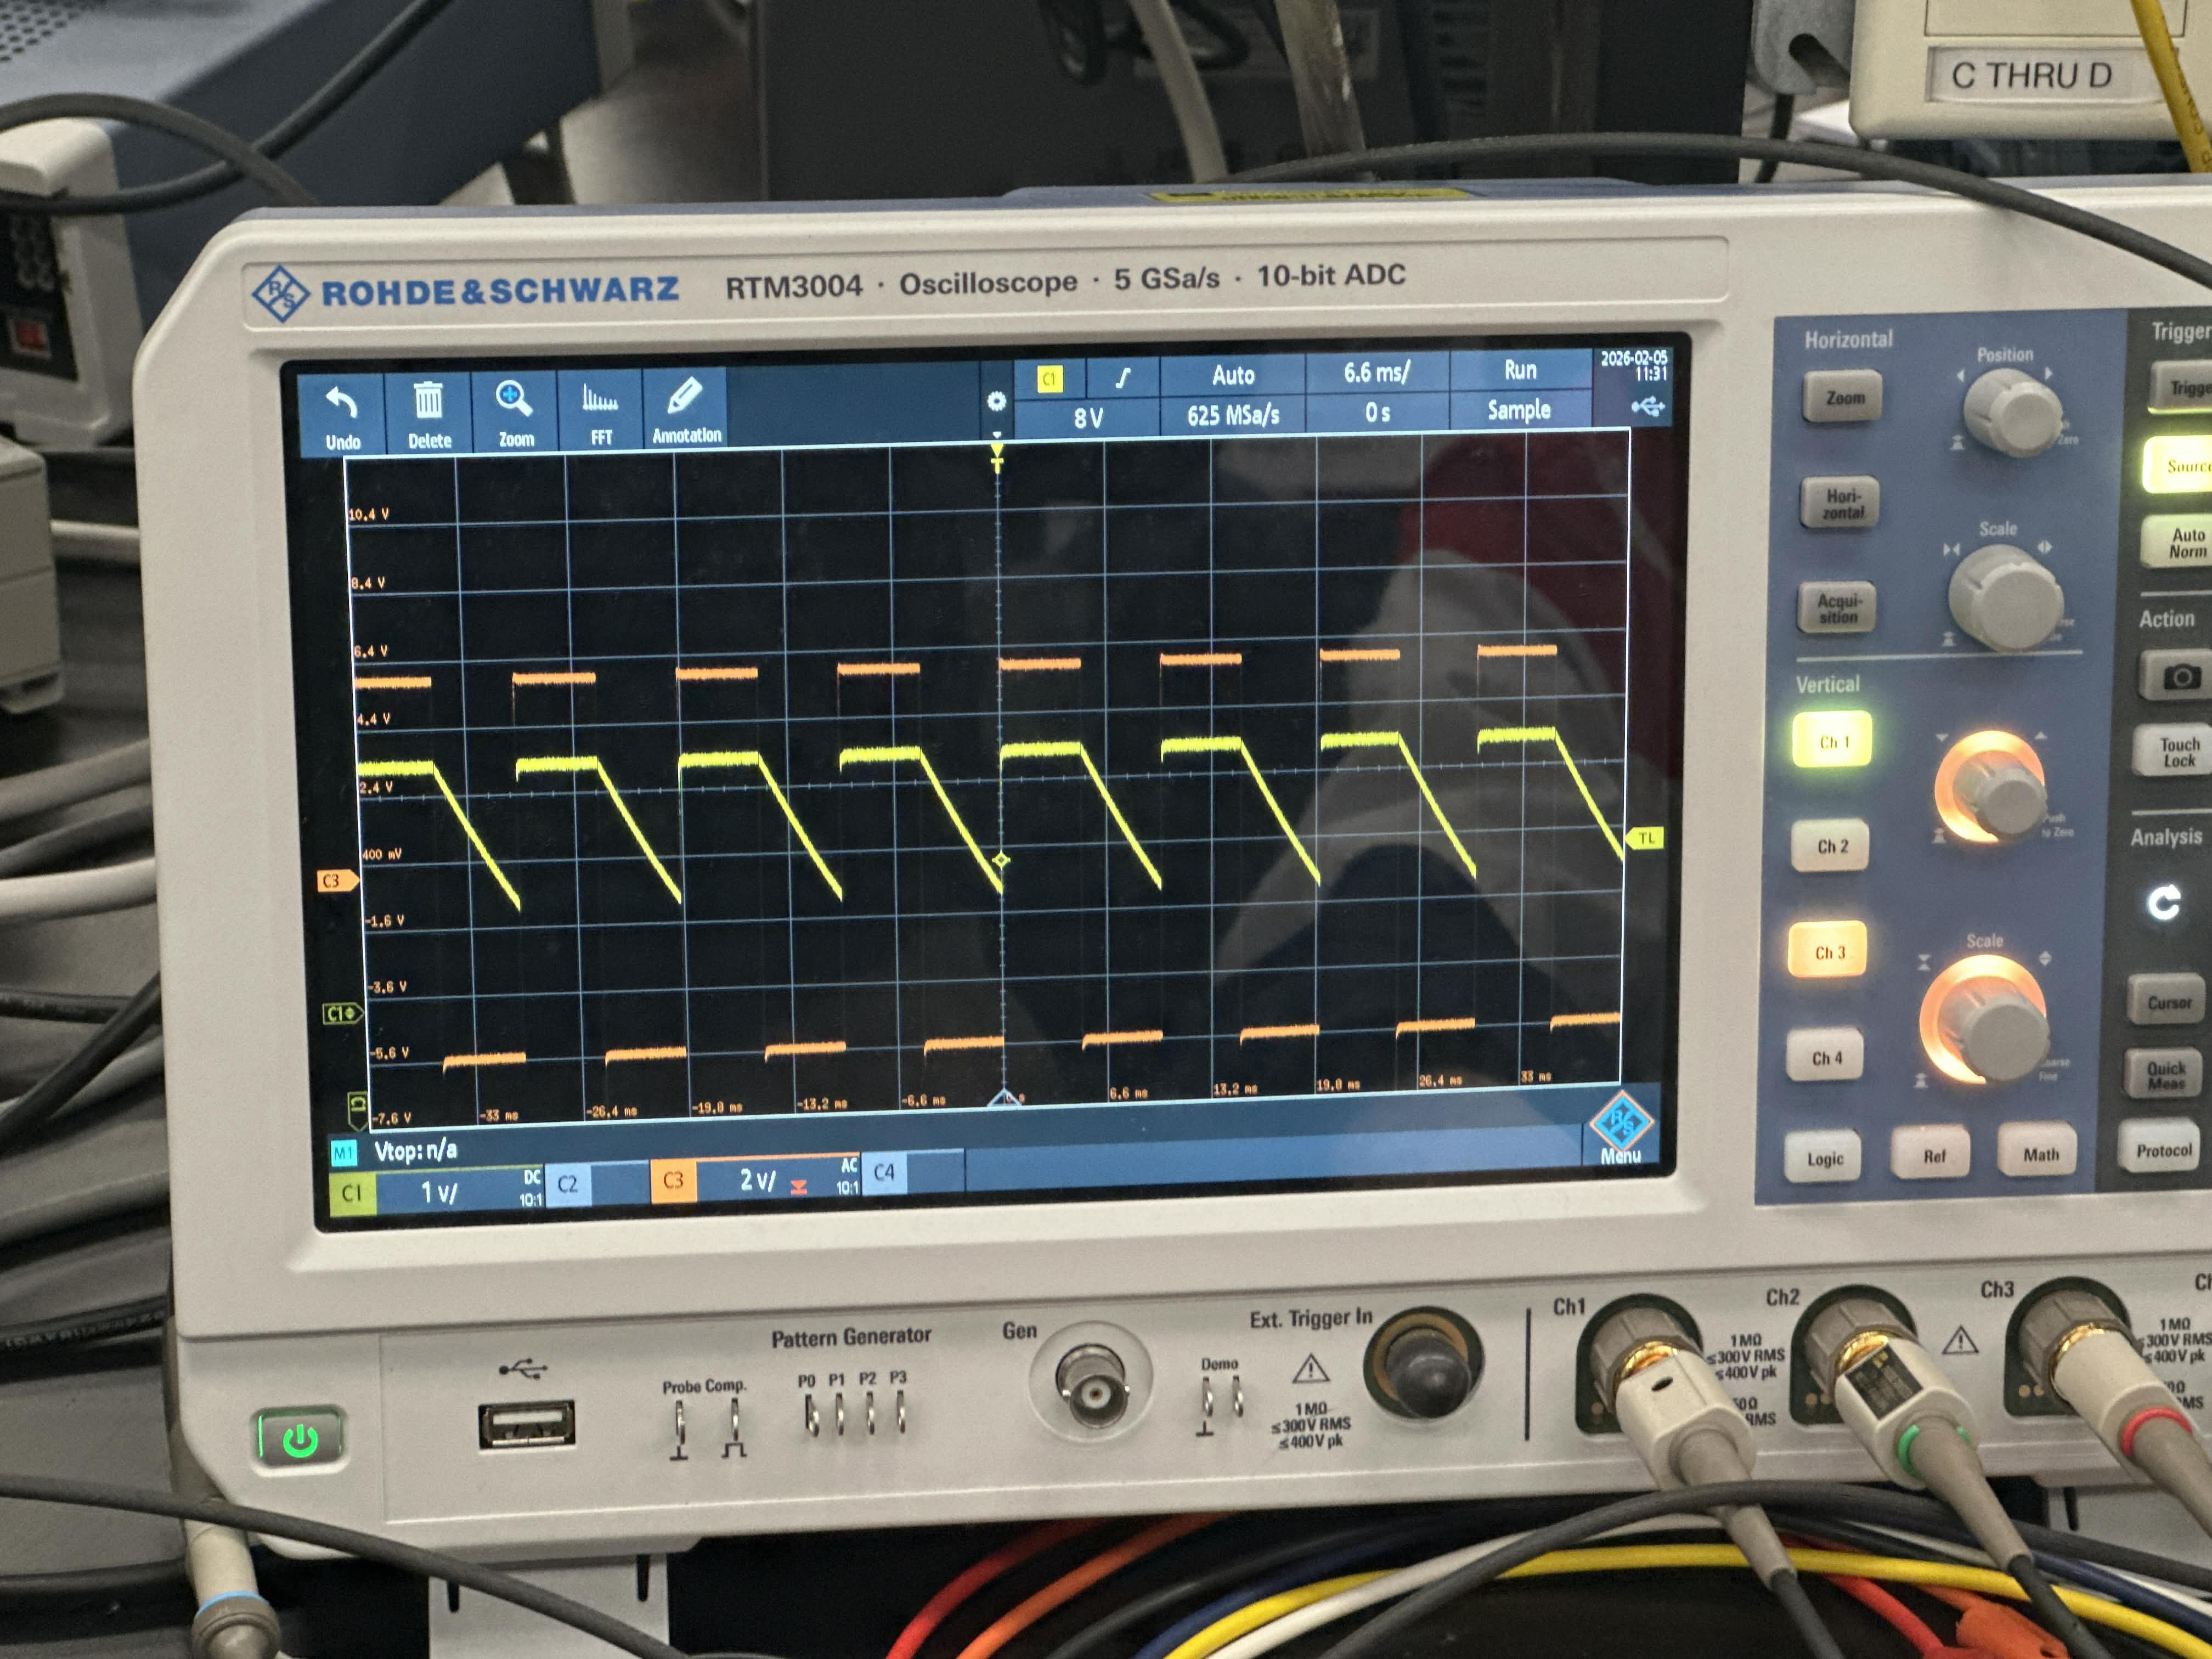
\includegraphics[width=\textwidth]{figure2_all_square.jpg}
		\caption{Square Input (Blue) vs Output (Yellow)}
		\label{fig:fw_all_square}
	\end{subfigure}
	\caption{Oscilloscope captures for the complete full-wave R-C-Diode peak rectifier.}
	\label{fig:fw_all_results}
\end{figure}

\textbf{Discussion:} \\
With all components in place, the full-wave peak rectifier produces a smoother DC output than its half-wave counterpart. Because the capacitor is recharged twice per input cycle, the ripple voltage is significantly reduced. The ripple frequency is twice the input frequency, and the peak-to-peak ripple is approximately half that of the half-wave configuration for the same $RC$ time constant.

\textbf{Calculation:}
Using the same component values ($R_L = 20\,\text{k}\Omega$, $C = 10\,\mu\text{F}$), the theoretical full-wave ripple is:
\[
V_{r(pp)} = \frac{V_p - V_{on}}{2f \cdot R_L \cdot C} = \frac{4.3}{200 \times 0.2} = \frac{4.3}{40} = 0.1075\,\text{V}
\]
Compared to the half-wave ripple of $0.215\,\text{V}$, the full-wave ripple is reduced by a factor of two ($0.1075 / 0.215 \approx 0.5$). This is consistent with the visibly smoother DC output observed in Figure~\ref{fig:fw_all_results}.

%-----------------------------------------
% CLIPPING CIRCUIT (Lab Manual Fig. 3)
%-----------------------------------------
\subsection{Clipping Circuit (Lab Manual Fig.~3)}
The clipping circuit limits the output voltage to a specified reference level. When the input exceeds this level, the diode conducts and clips the waveform.

\begin{figure}[H]
	\centering
	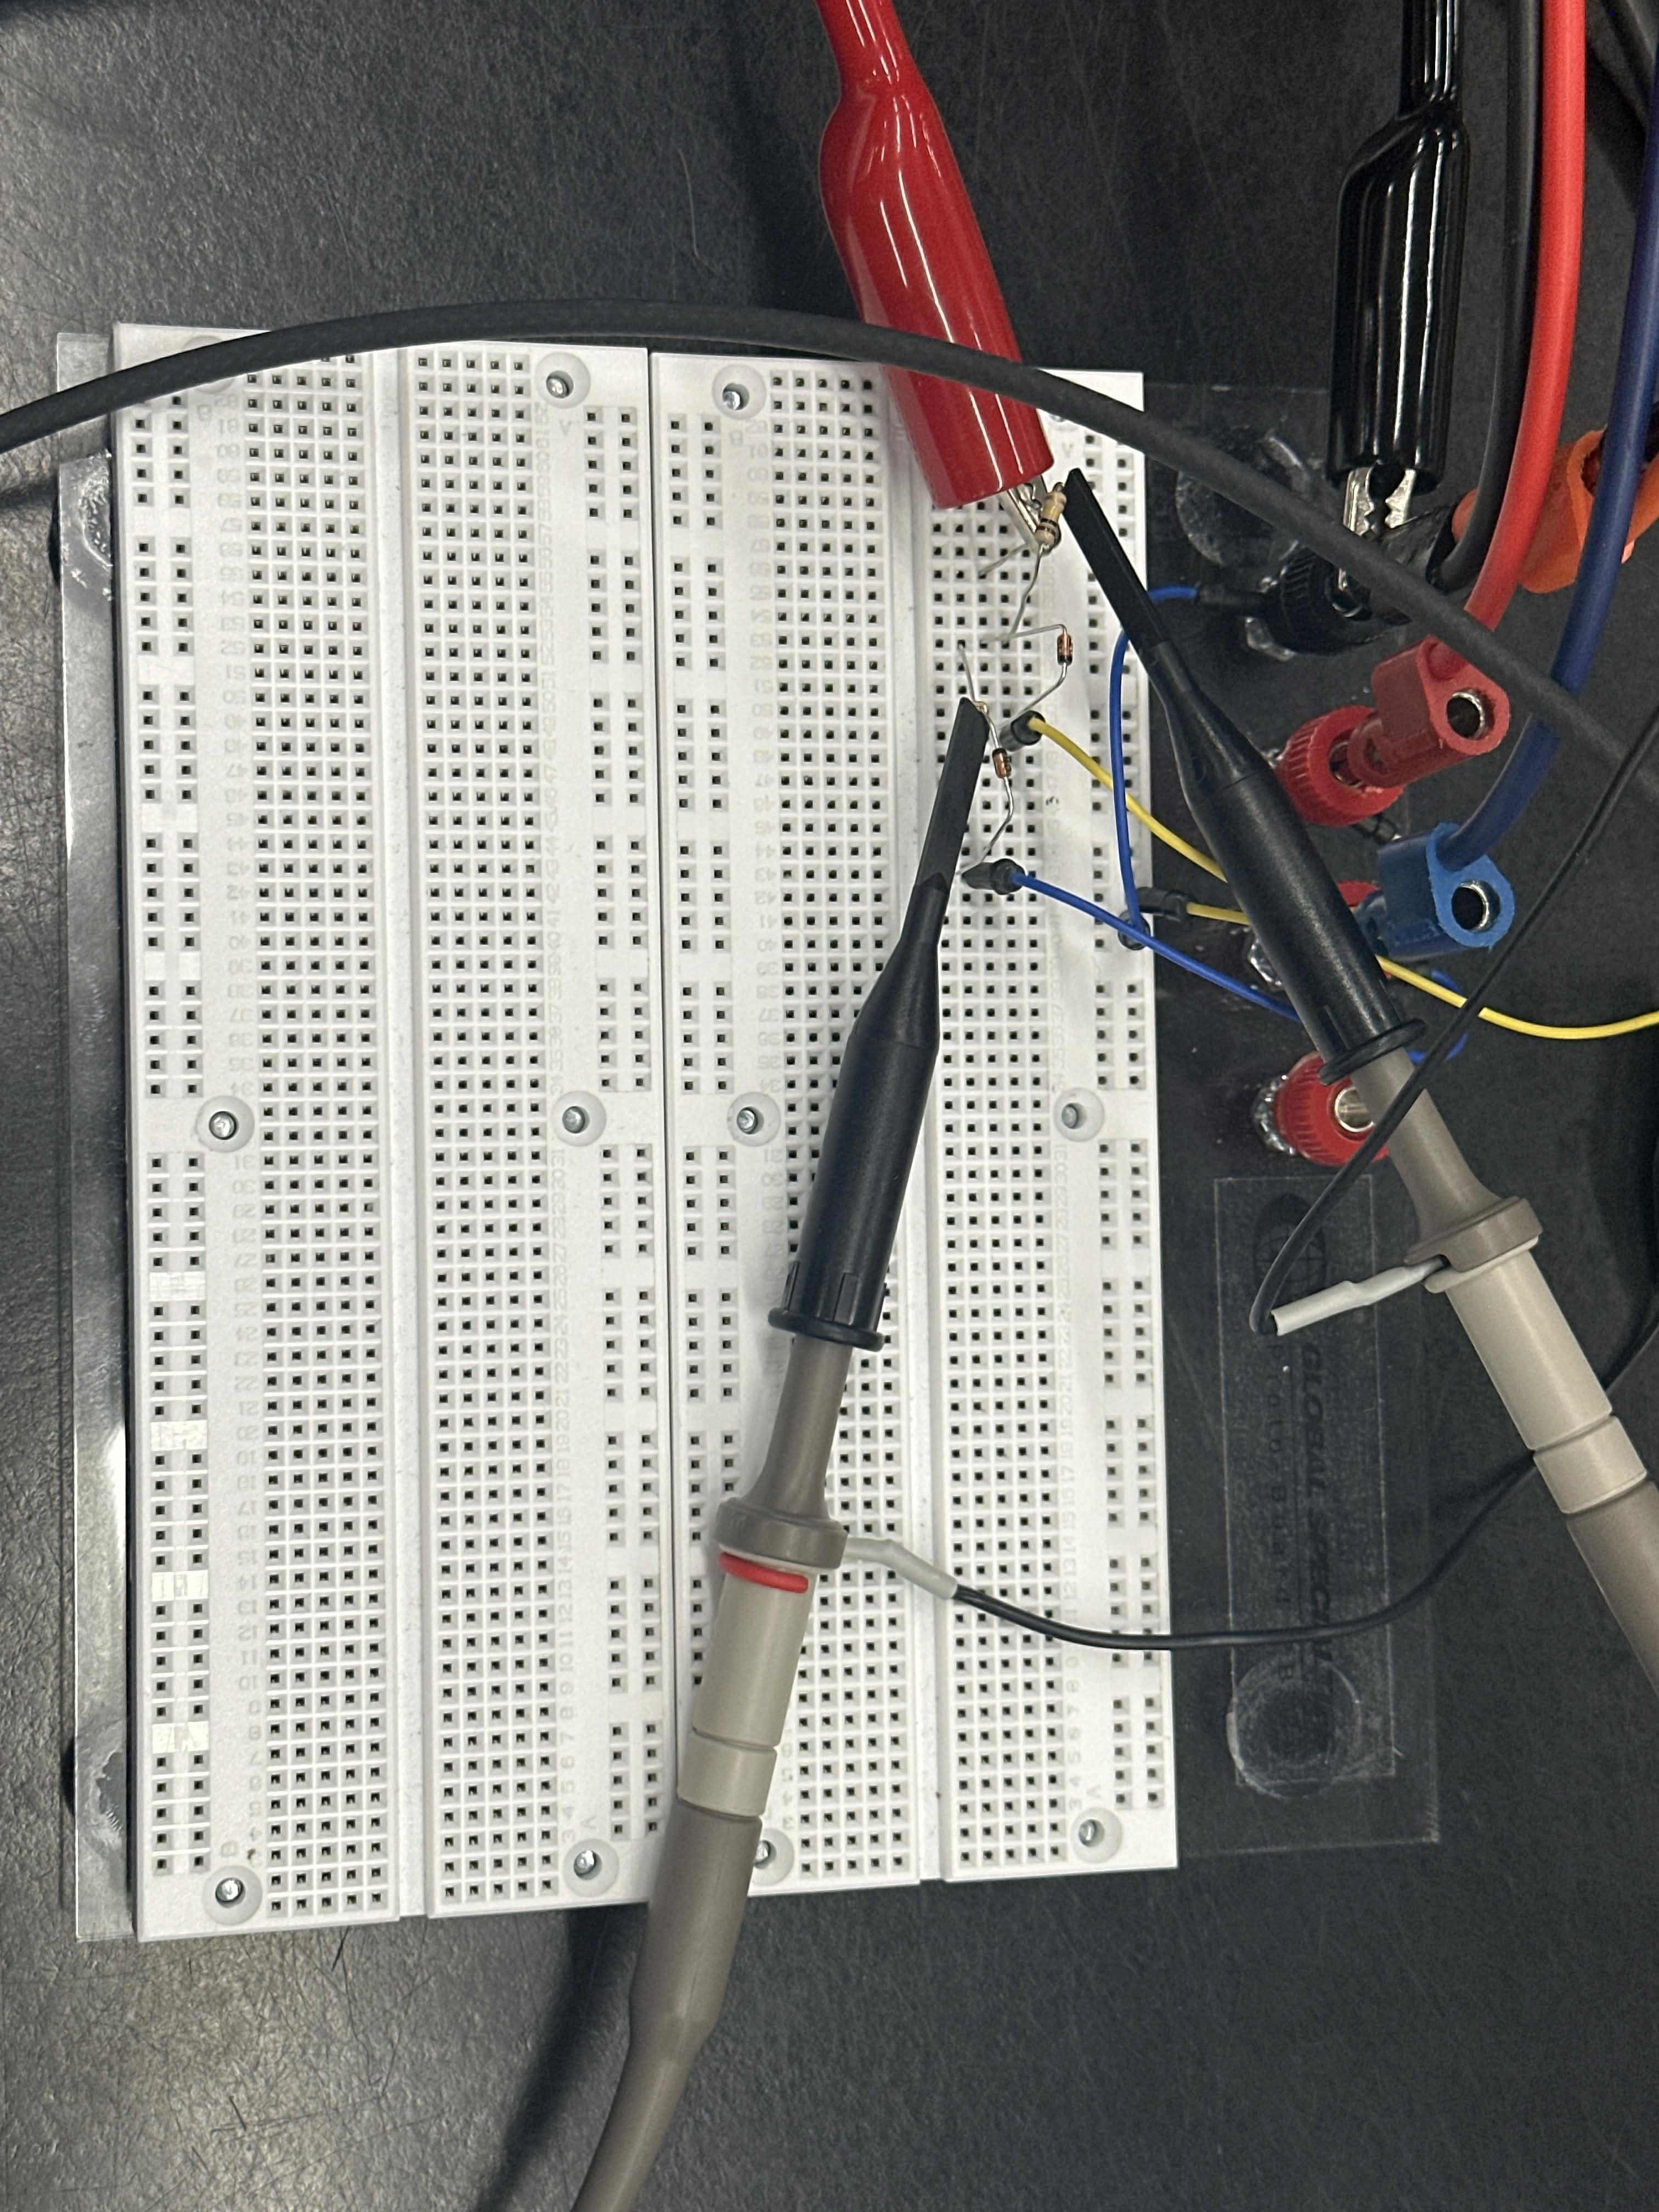
\includegraphics[width=0.5\textwidth,angle=90]{figure3.jpg}
	\caption{Breadboard of the clipping circuit.}
	\label{fig:hand_drawn_3}
\end{figure}

\begin{figure}[H]
	\centering
	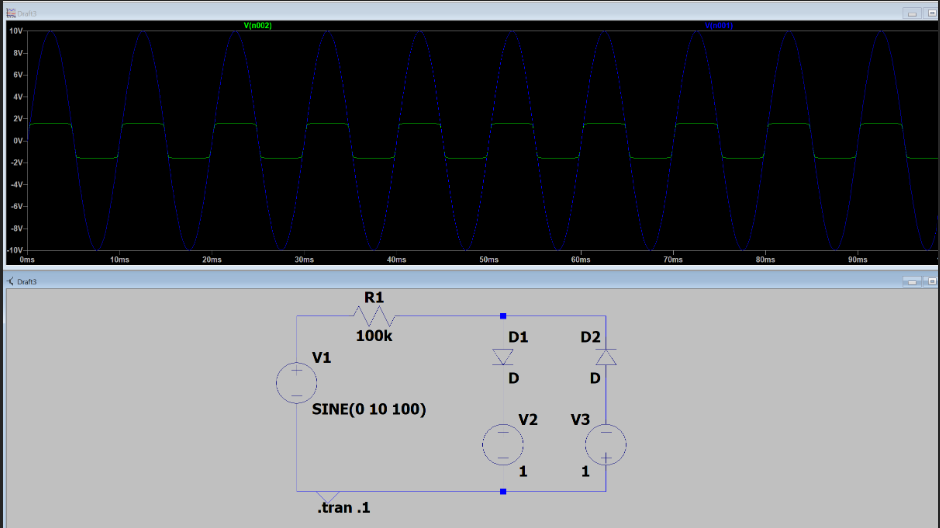
\includegraphics[width=0.6\textwidth]{figure3_ltspice.png}
	\caption{LTspice simulation schematic for the clipping circuit.}
	\label{fig:clip_sch}
\end{figure}

\begin{figure}[H]
	\centering
	\begin{subfigure}[b]{0.48\textwidth}
		\centering
		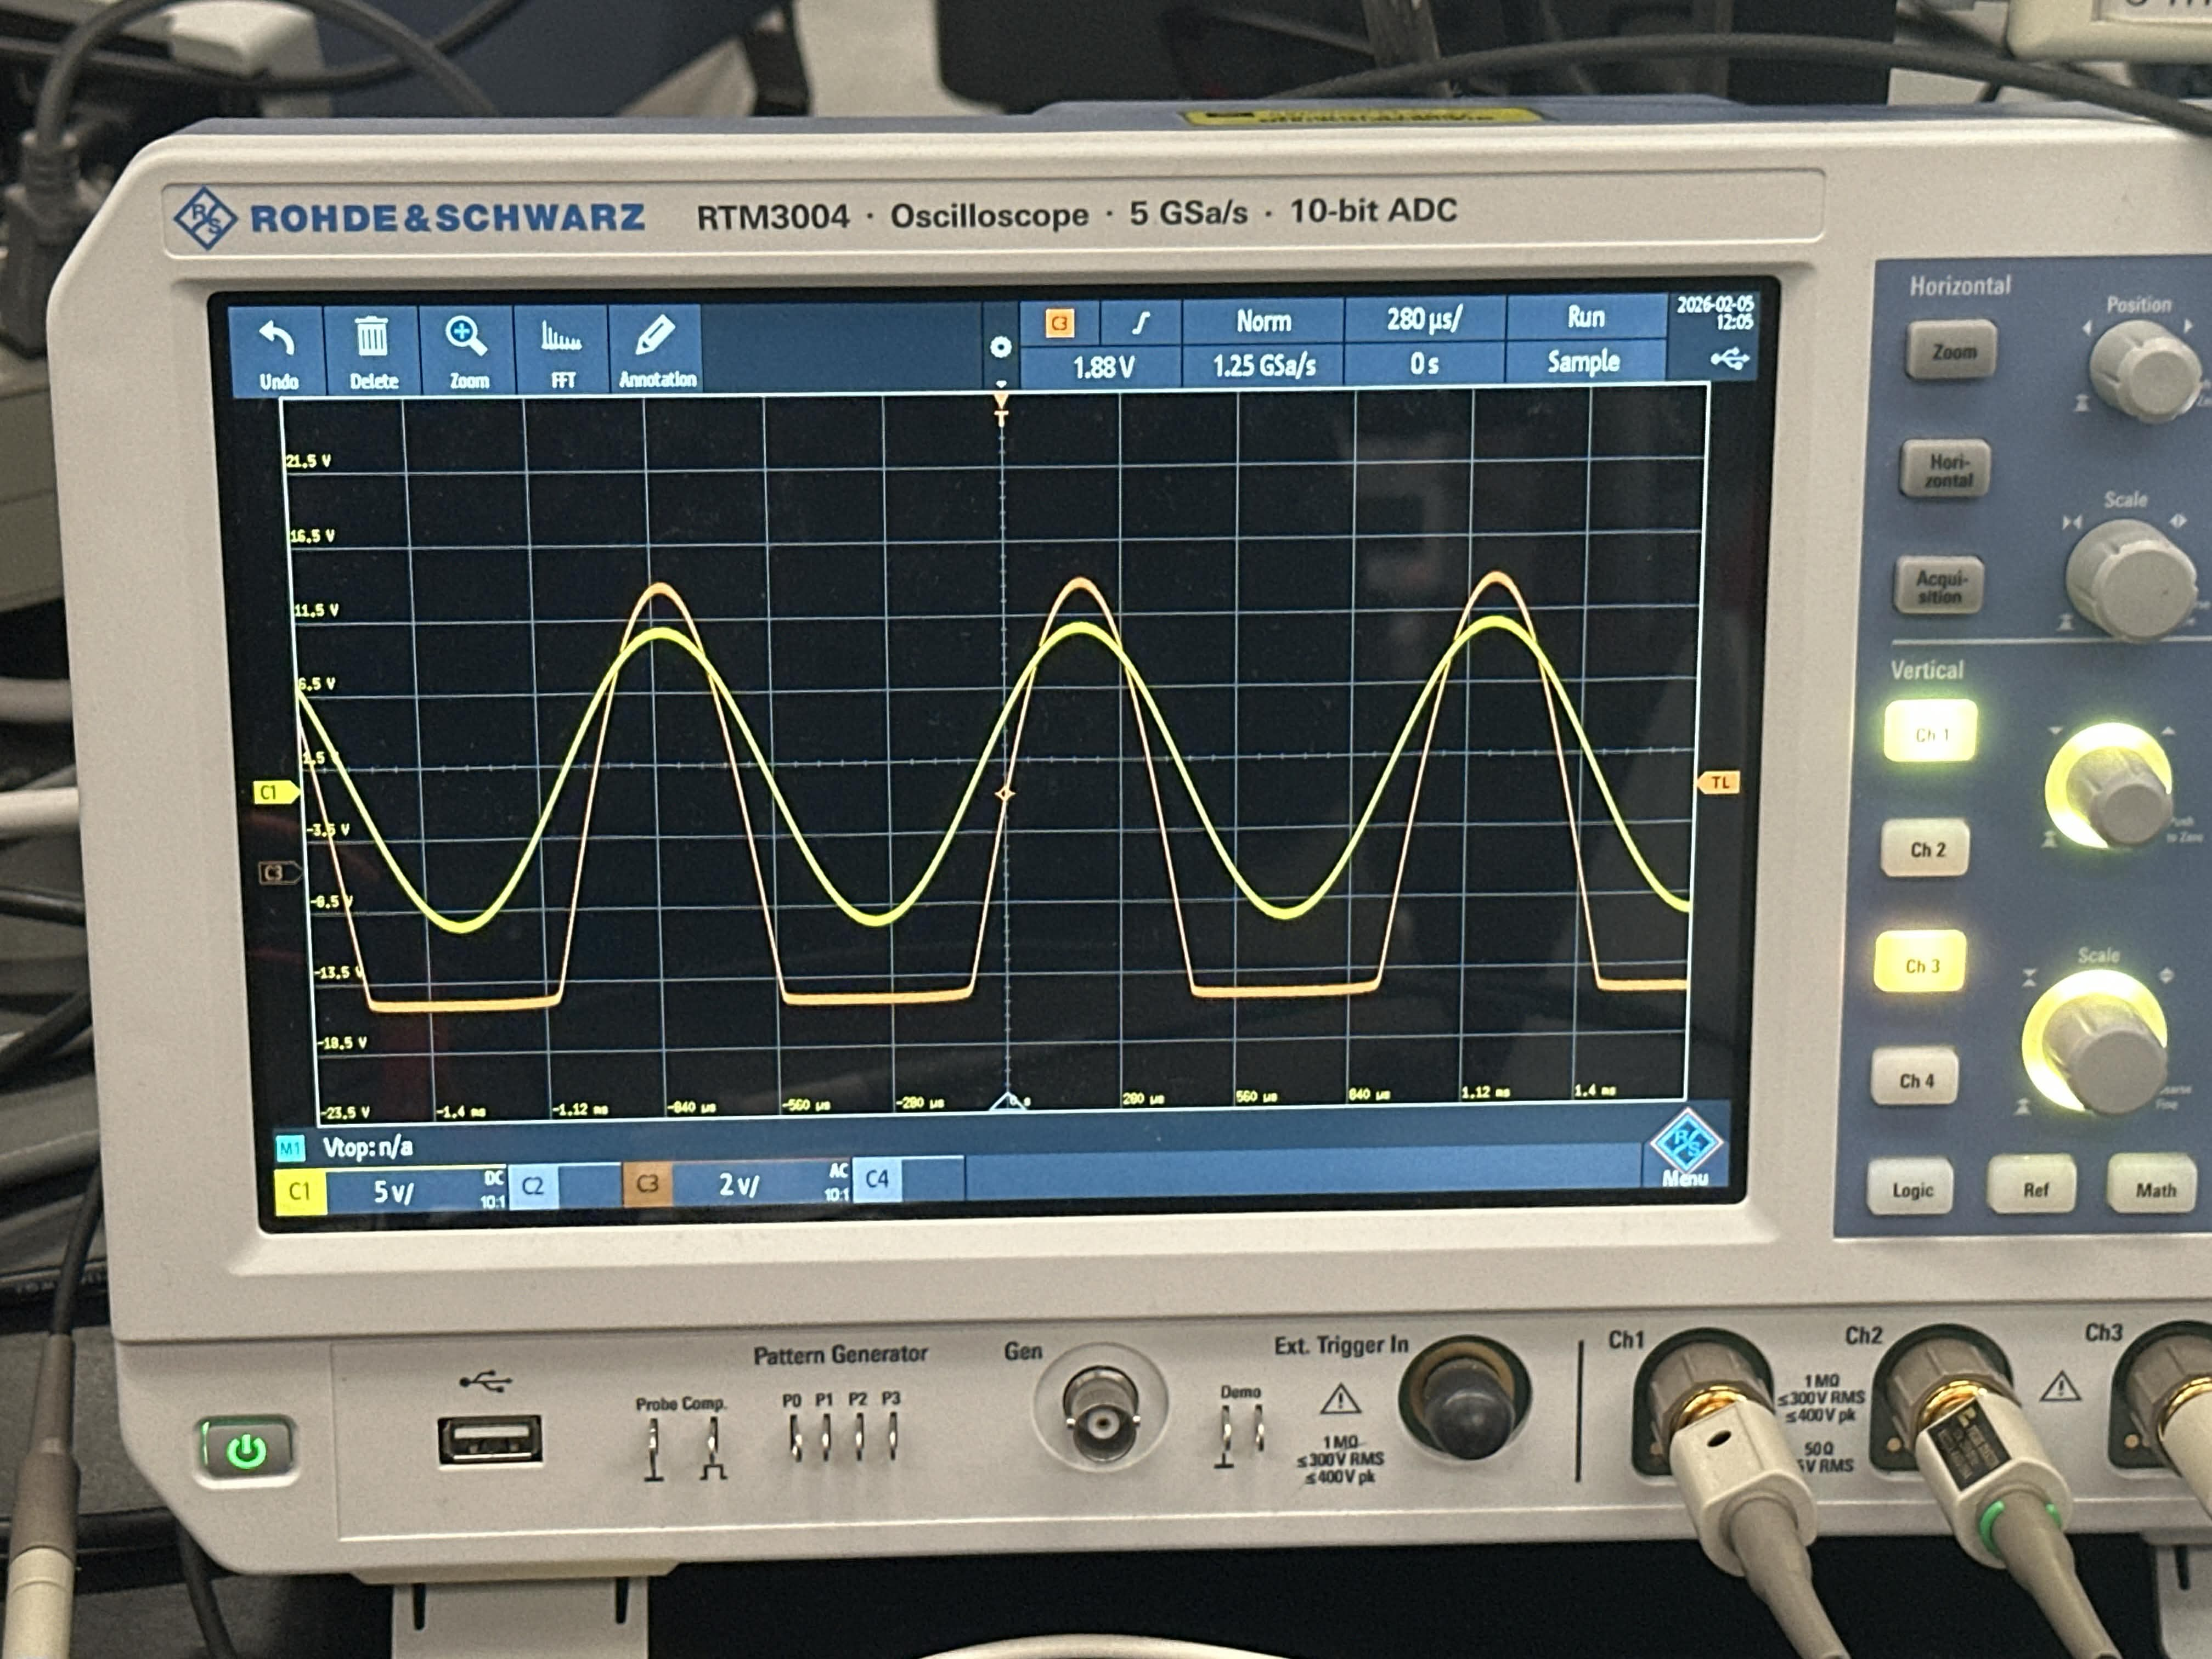
\includegraphics[width=\textwidth]{figure3_sine.jpg}
		\caption{Sinusoidal Input (Blue) vs Output (Yellow)}
		\label{fig:clip_sine}
	\end{subfigure}
	\hfill
	\begin{subfigure}[b]{0.48\textwidth}
		\centering
		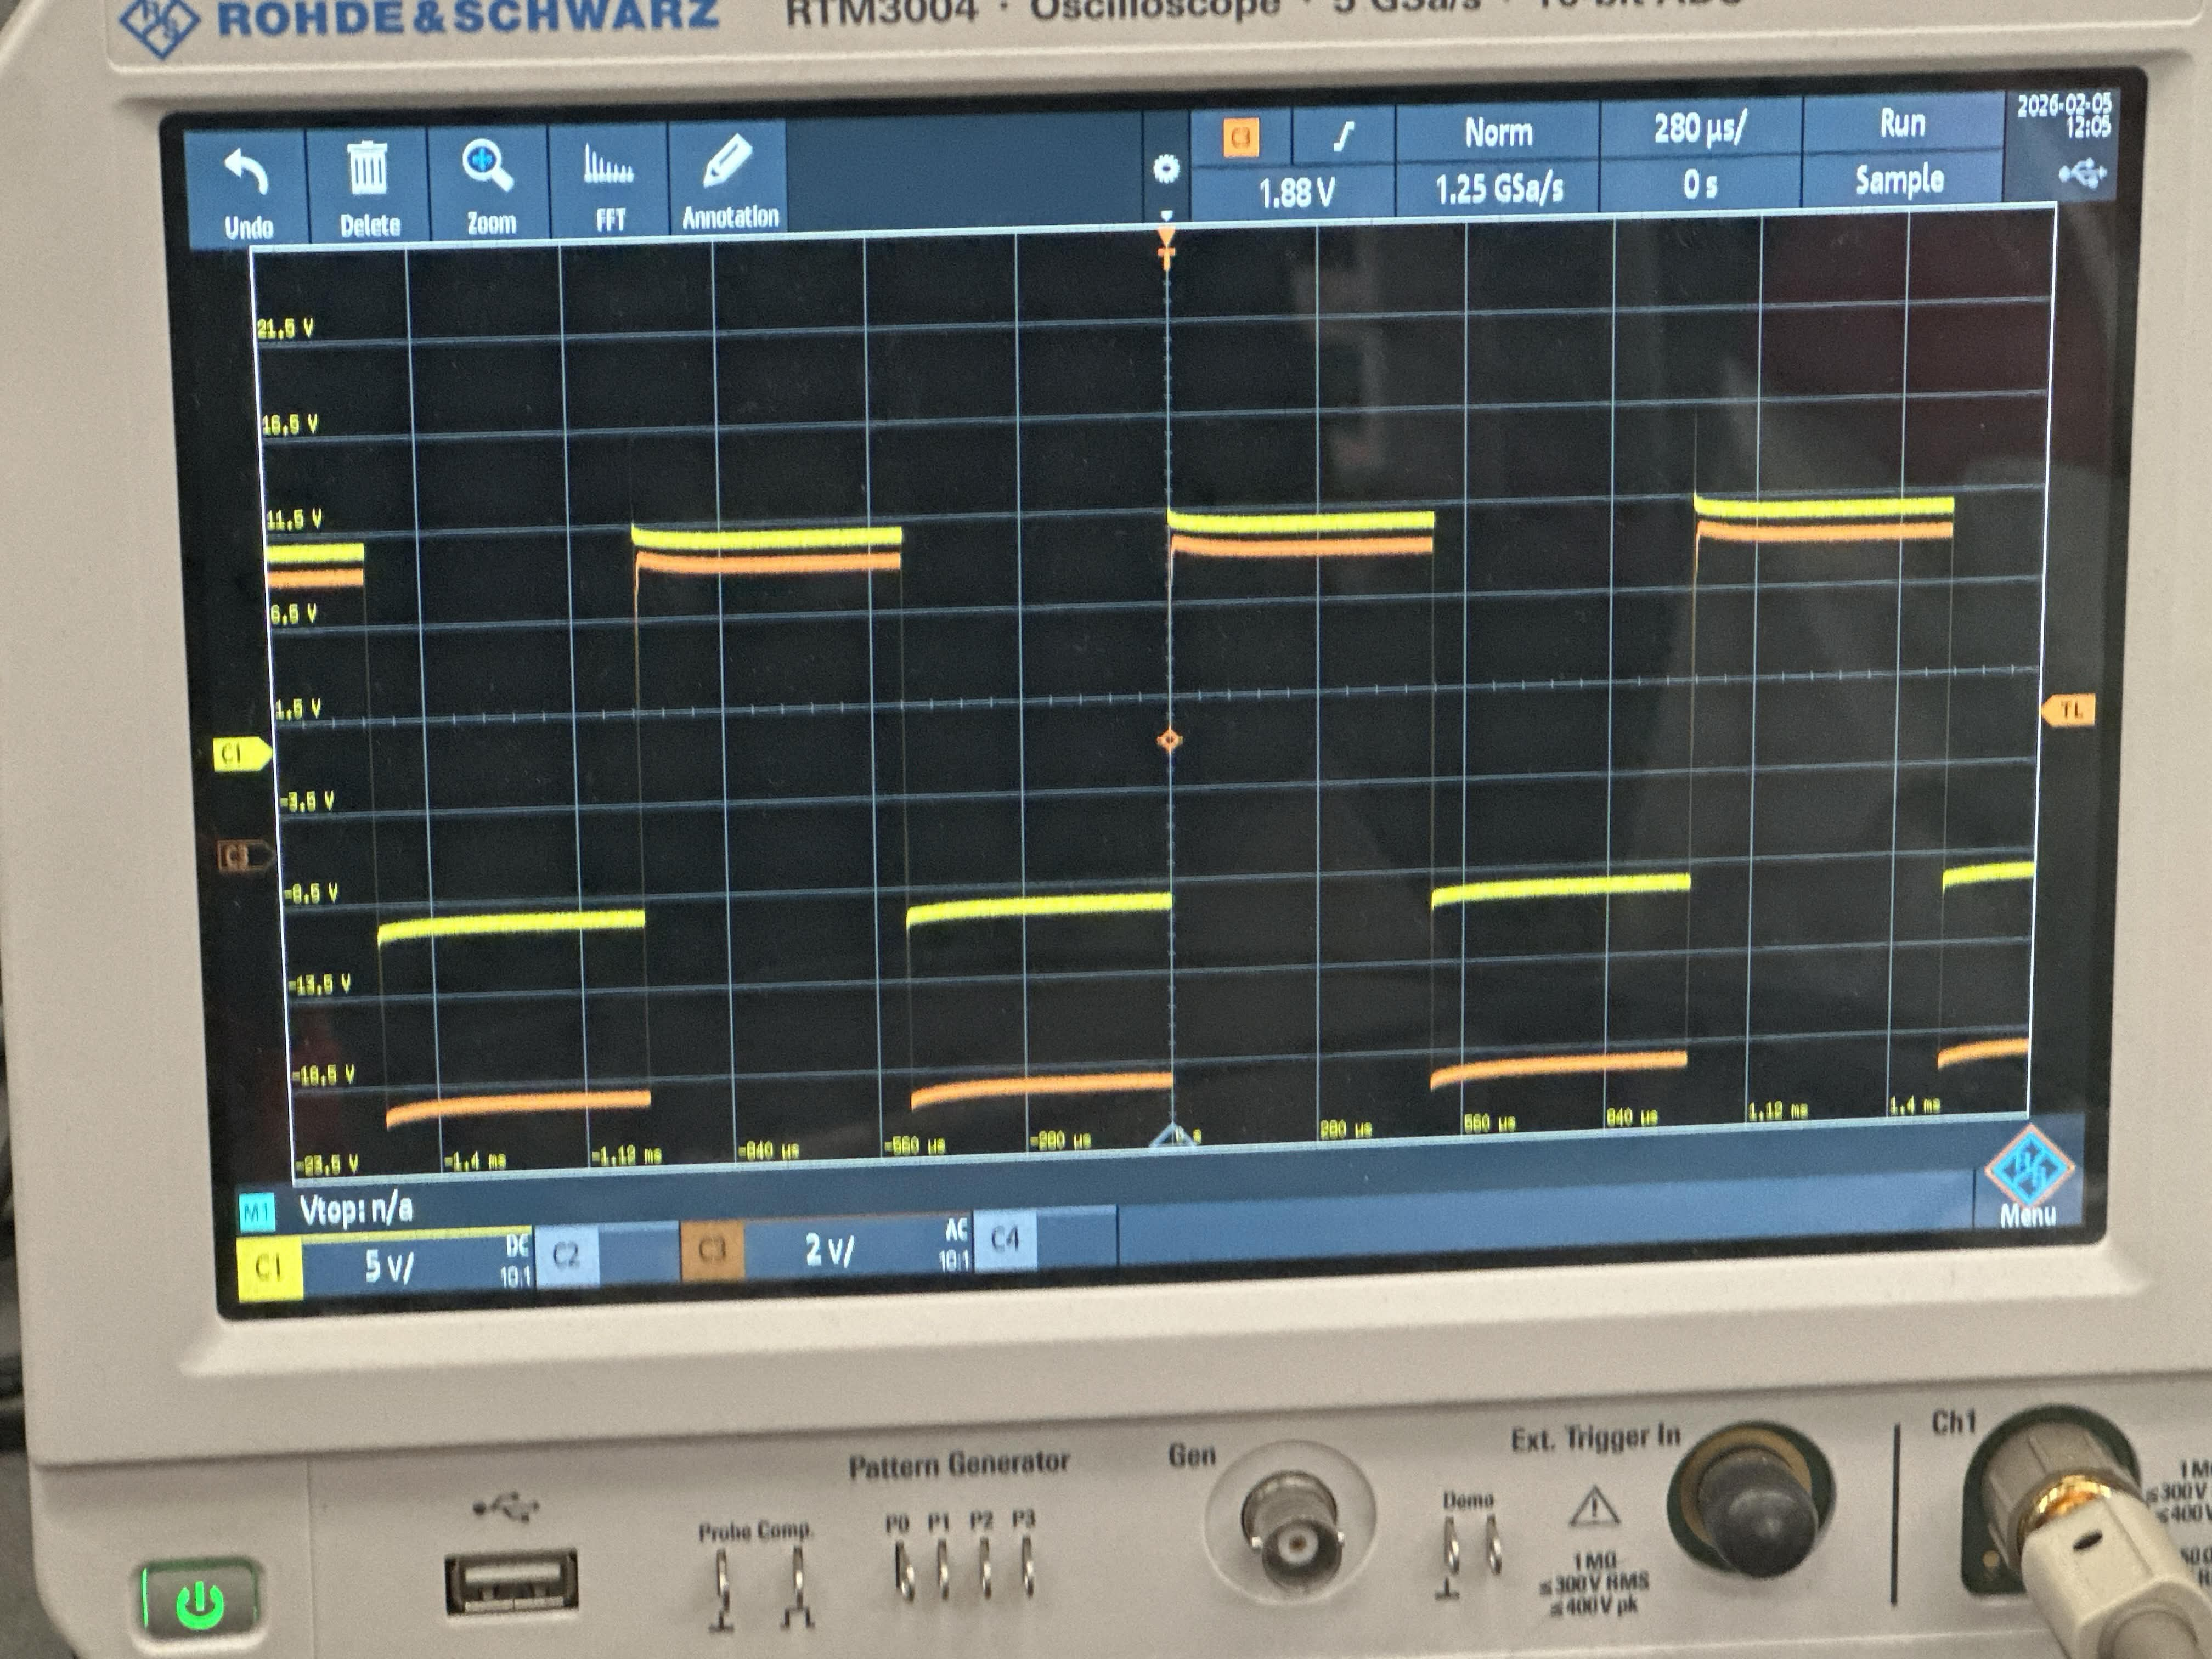
\includegraphics[width=\textwidth]{figure3_square.jpg}
		\caption{Square Input (Blue) vs Output (Yellow)}
		\label{fig:clip_square}
	\end{subfigure}
	\caption{Oscilloscope captures for the clipping circuit.}
	\label{fig:clip_results}
\end{figure}

\textbf{Discussion:} \\
The clipping circuit effectively limits the output voltage. When the input exceeds the reference voltage plus the diode turn-on voltage, the diode conducts and the output is clamped at that threshold. When the input is below the threshold, the output follows the input directly. The clipped portions of the sine and square waves are clearly visible in Figure~\ref{fig:clip_results}.

\textbf{Calculation:}
The clipping threshold is determined by:
\[
V_{clip} = V_{ref} + V_{on}
\]
For input amplitudes below $V_{clip}$, the output follows the input identically (no clipping). As the input amplitude was increased beyond $V_{clip}$, the clipped portion of each cycle widened, confirming the onset of diode conduction at the expected threshold. Conversely, when the amplitude was reduced below $V_{clip}$, the output tracked the input without any clipping, as predicted by the transfer characteristic.

%-----------------------------------------
% ZENER CLIPPING CIRCUIT (Lab Manual Fig. 4)
%-----------------------------------------
\subsection{Zener Clipping Circuit (Lab Manual Fig.~4)}
This circuit uses two back-to-back Zener diodes (1N5234, $V_Z \approx 6.2\,\text{V}$) to symmetrically clip both the positive and negative peaks of the input waveform.

\begin{figure}[H]
	\centering
	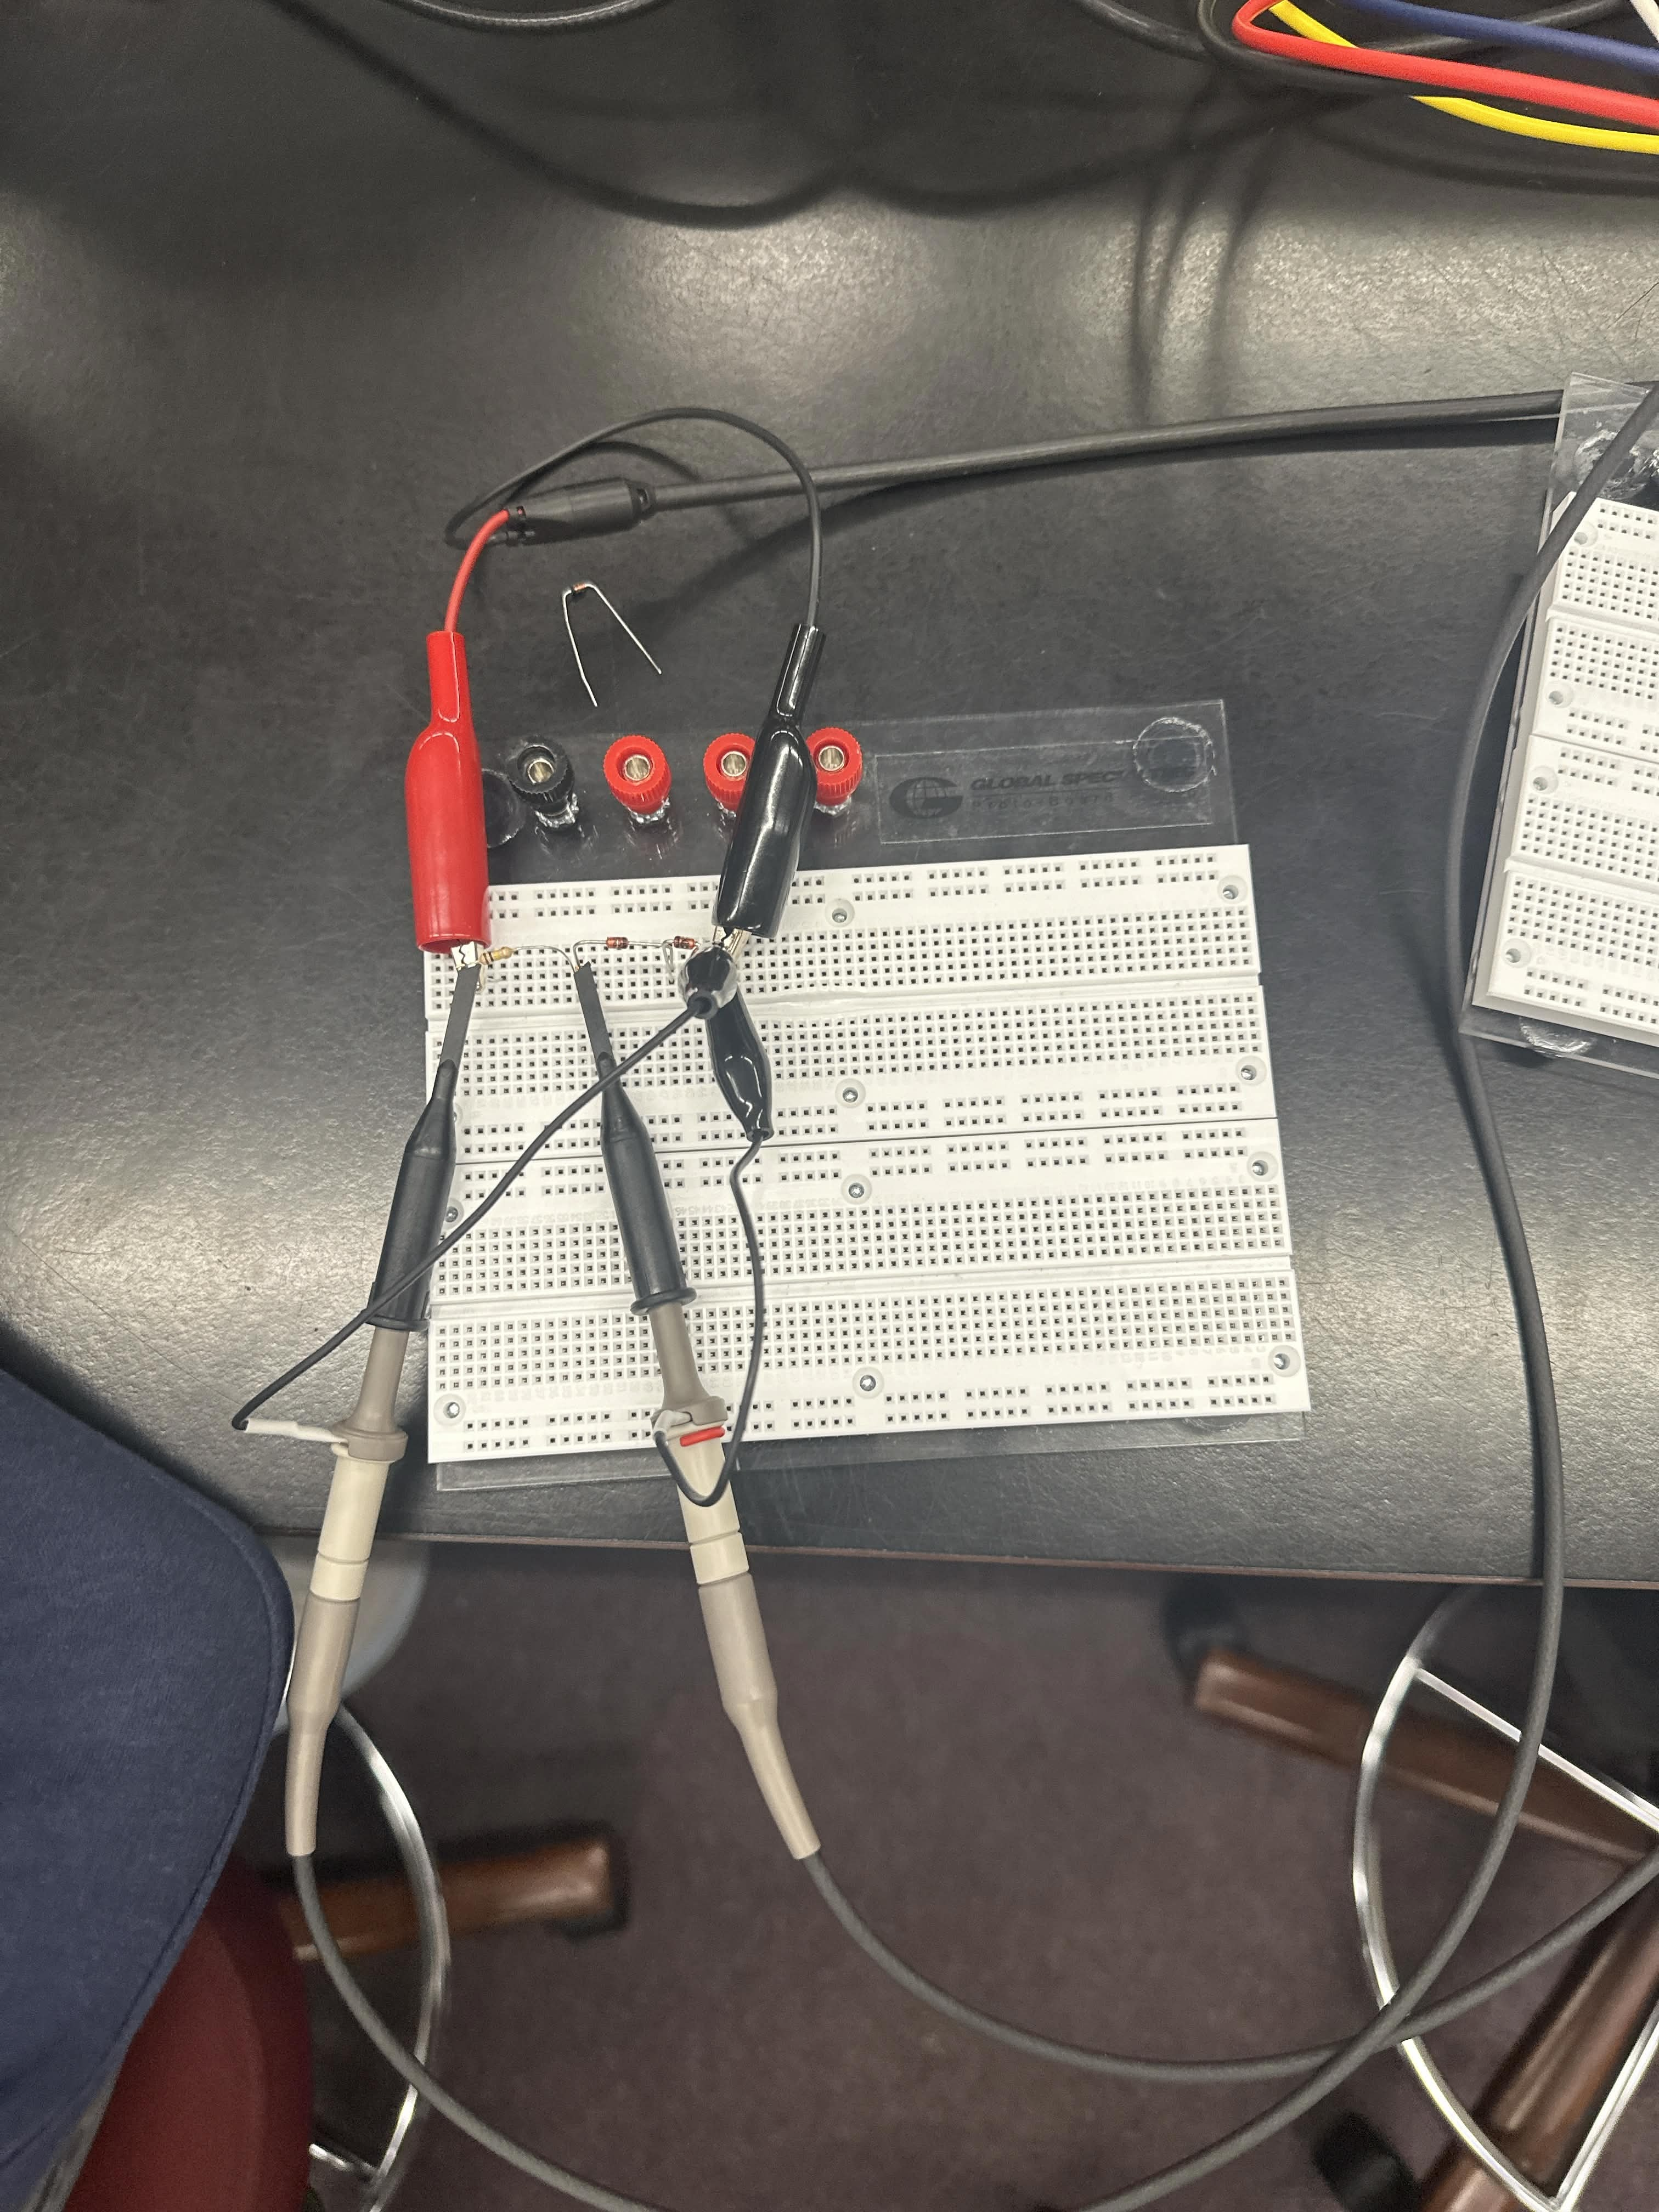
\includegraphics[width=0.6\textwidth]{figure4.jpg}
	\caption{Breadboard of the Zener clipping circuit.}
	\label{fig:hand_drawn_4}
\end{figure}

\begin{figure}[H]
	\centering
	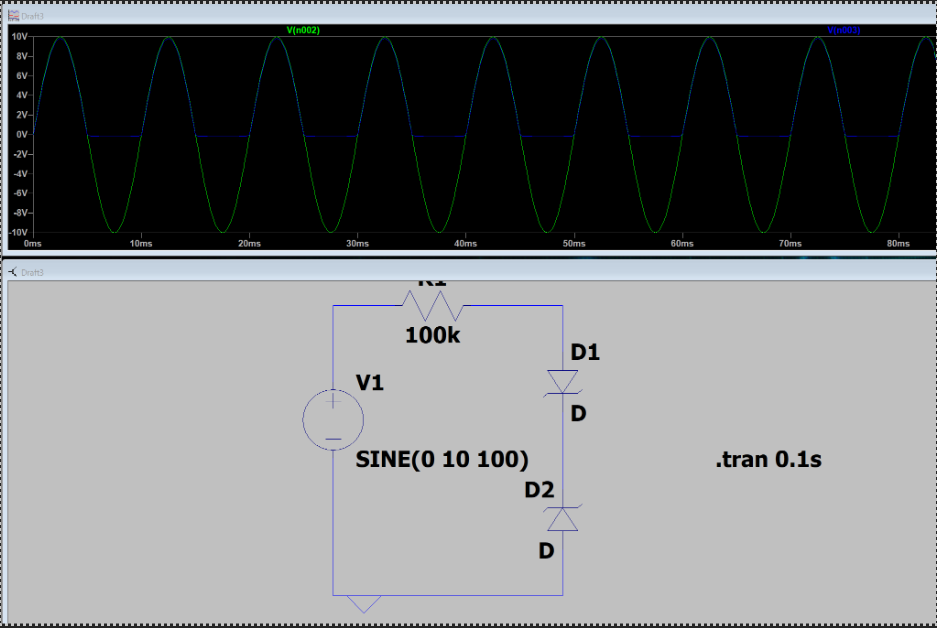
\includegraphics[width=0.6\textwidth]{figure4_ltspice.png}
	\caption{LTspice simulation schematic for the Zener clipping circuit.}
	\label{fig:zener_sch}
\end{figure}

\begin{figure}[H]
	\centering
	\begin{subfigure}[b]{0.48\textwidth}
		\centering
		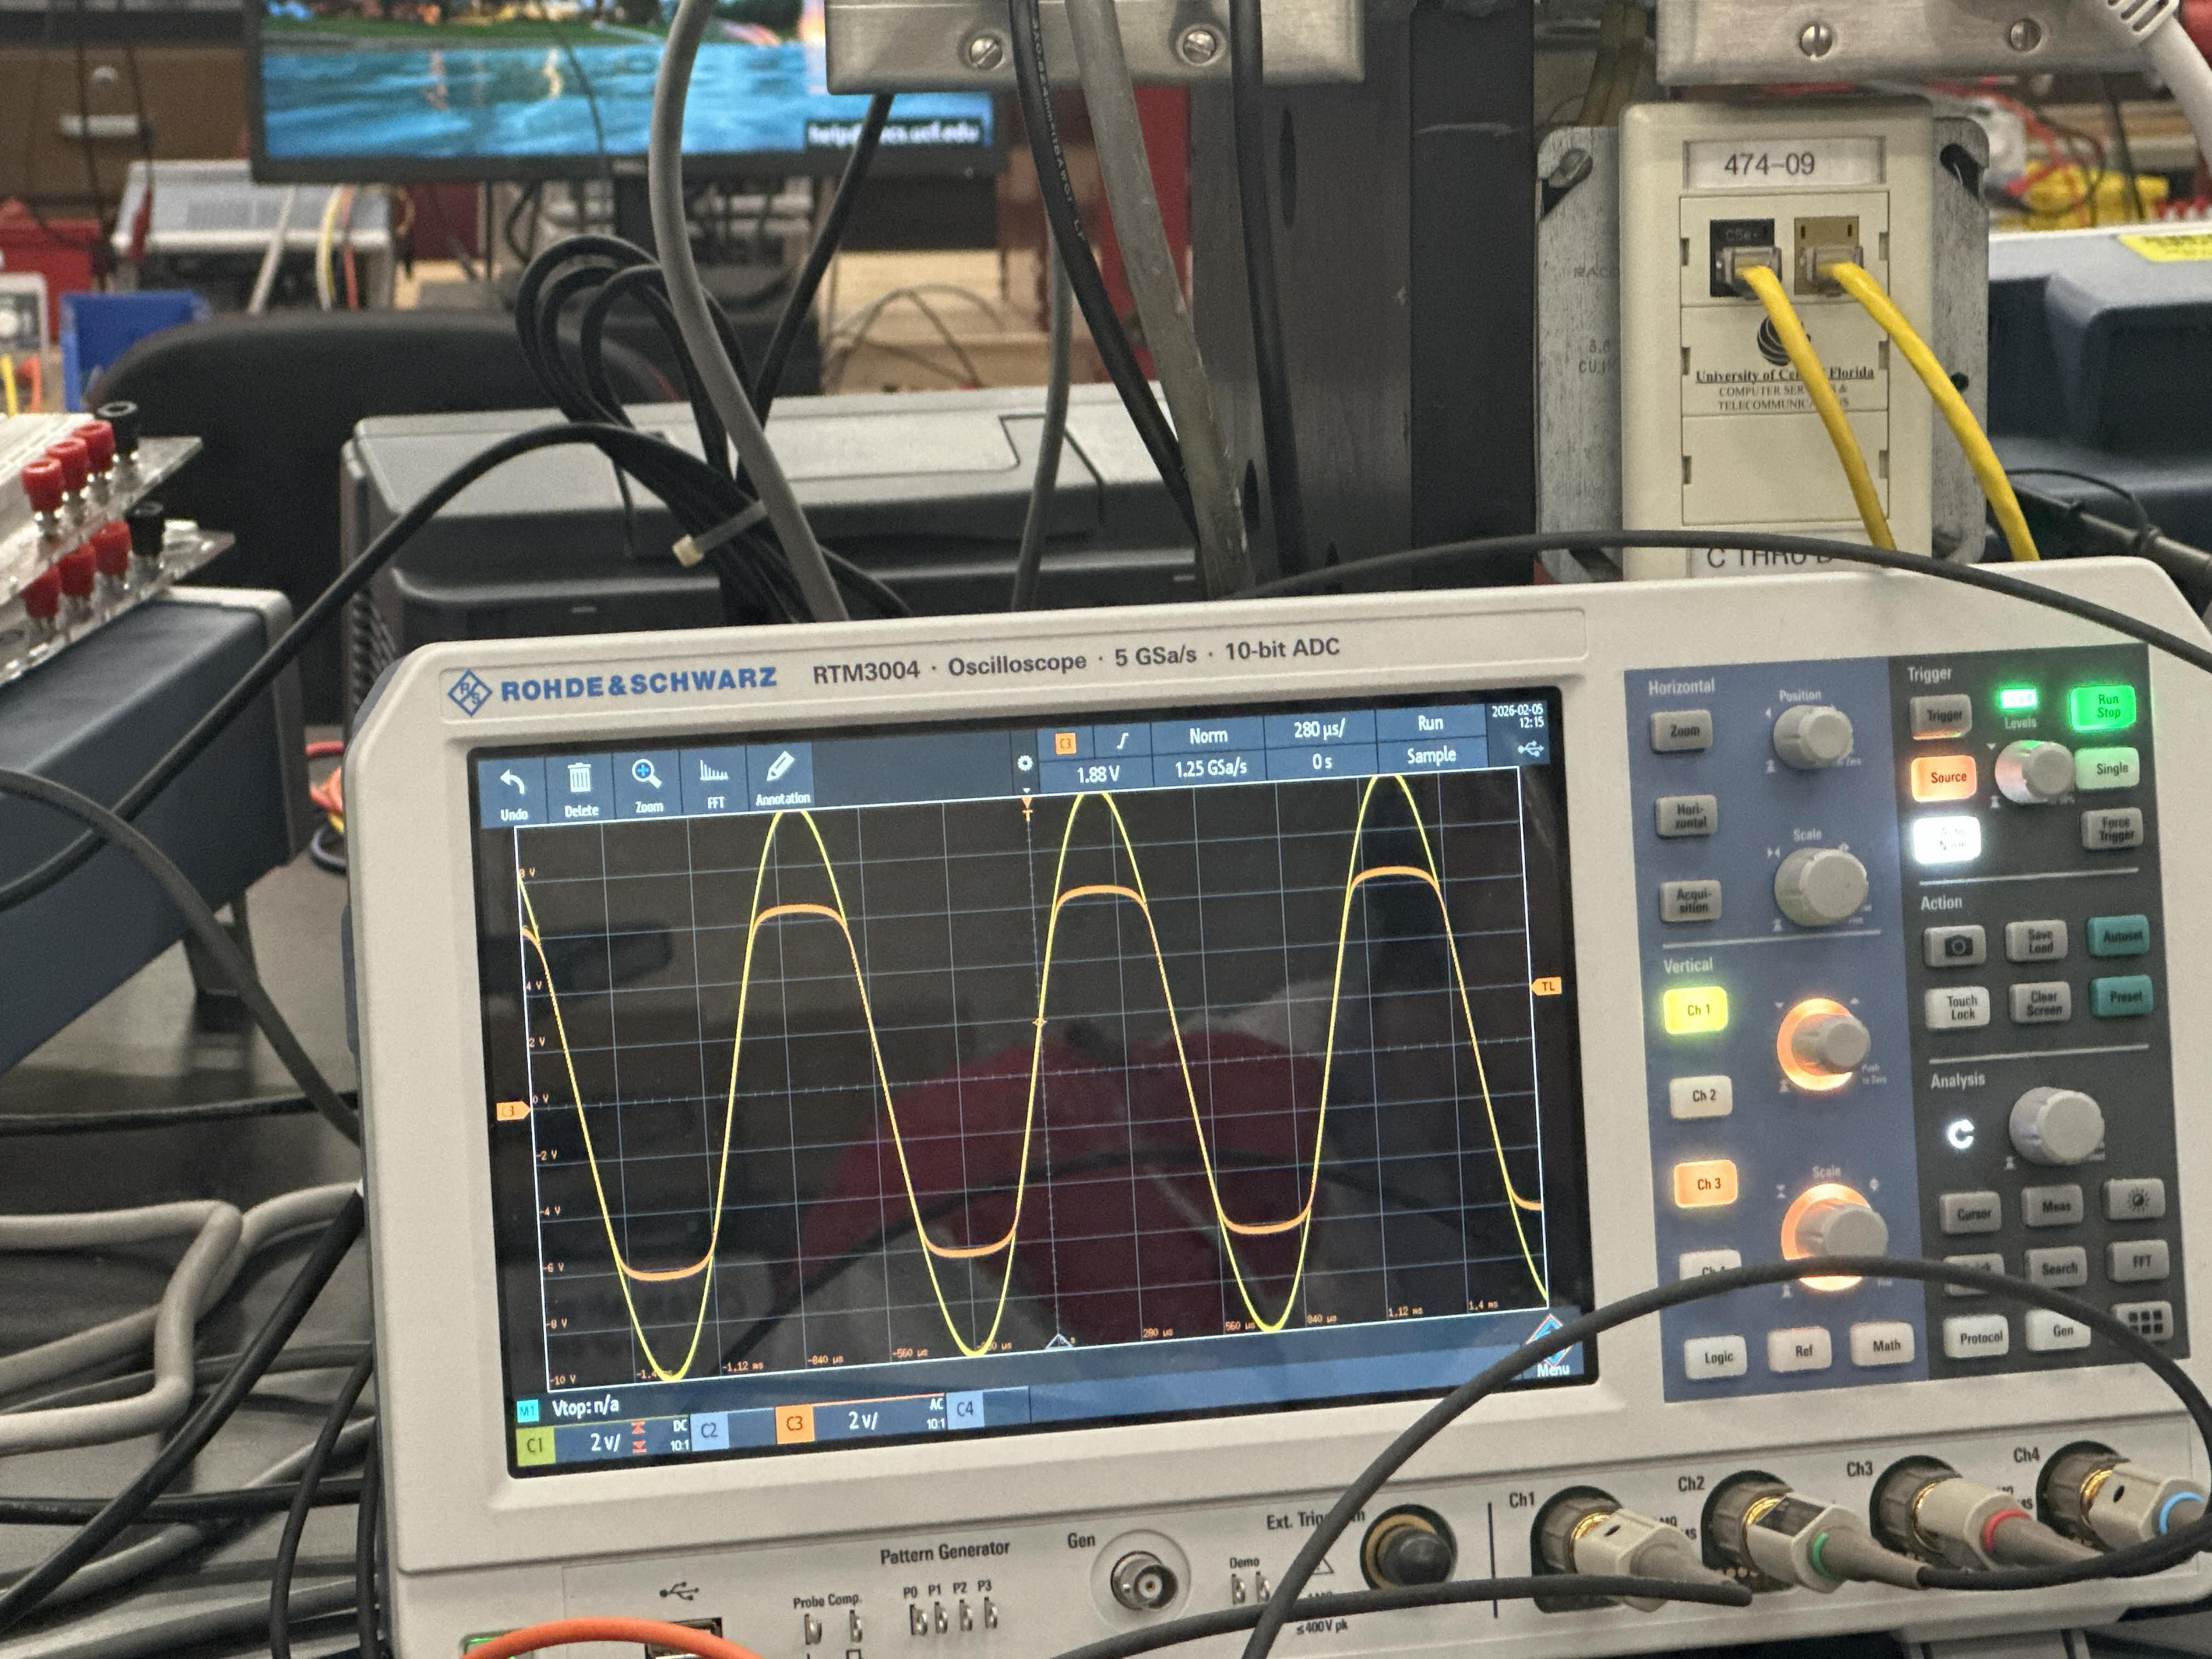
\includegraphics[width=\textwidth]{figure4_sine.jpg}
		\caption{Sinusoidal Input (Blue) vs Output (Yellow)}
		\label{fig:zener_sine}
	\end{subfigure}
	\hfill
	\begin{subfigure}[b]{0.48\textwidth}
		\centering
		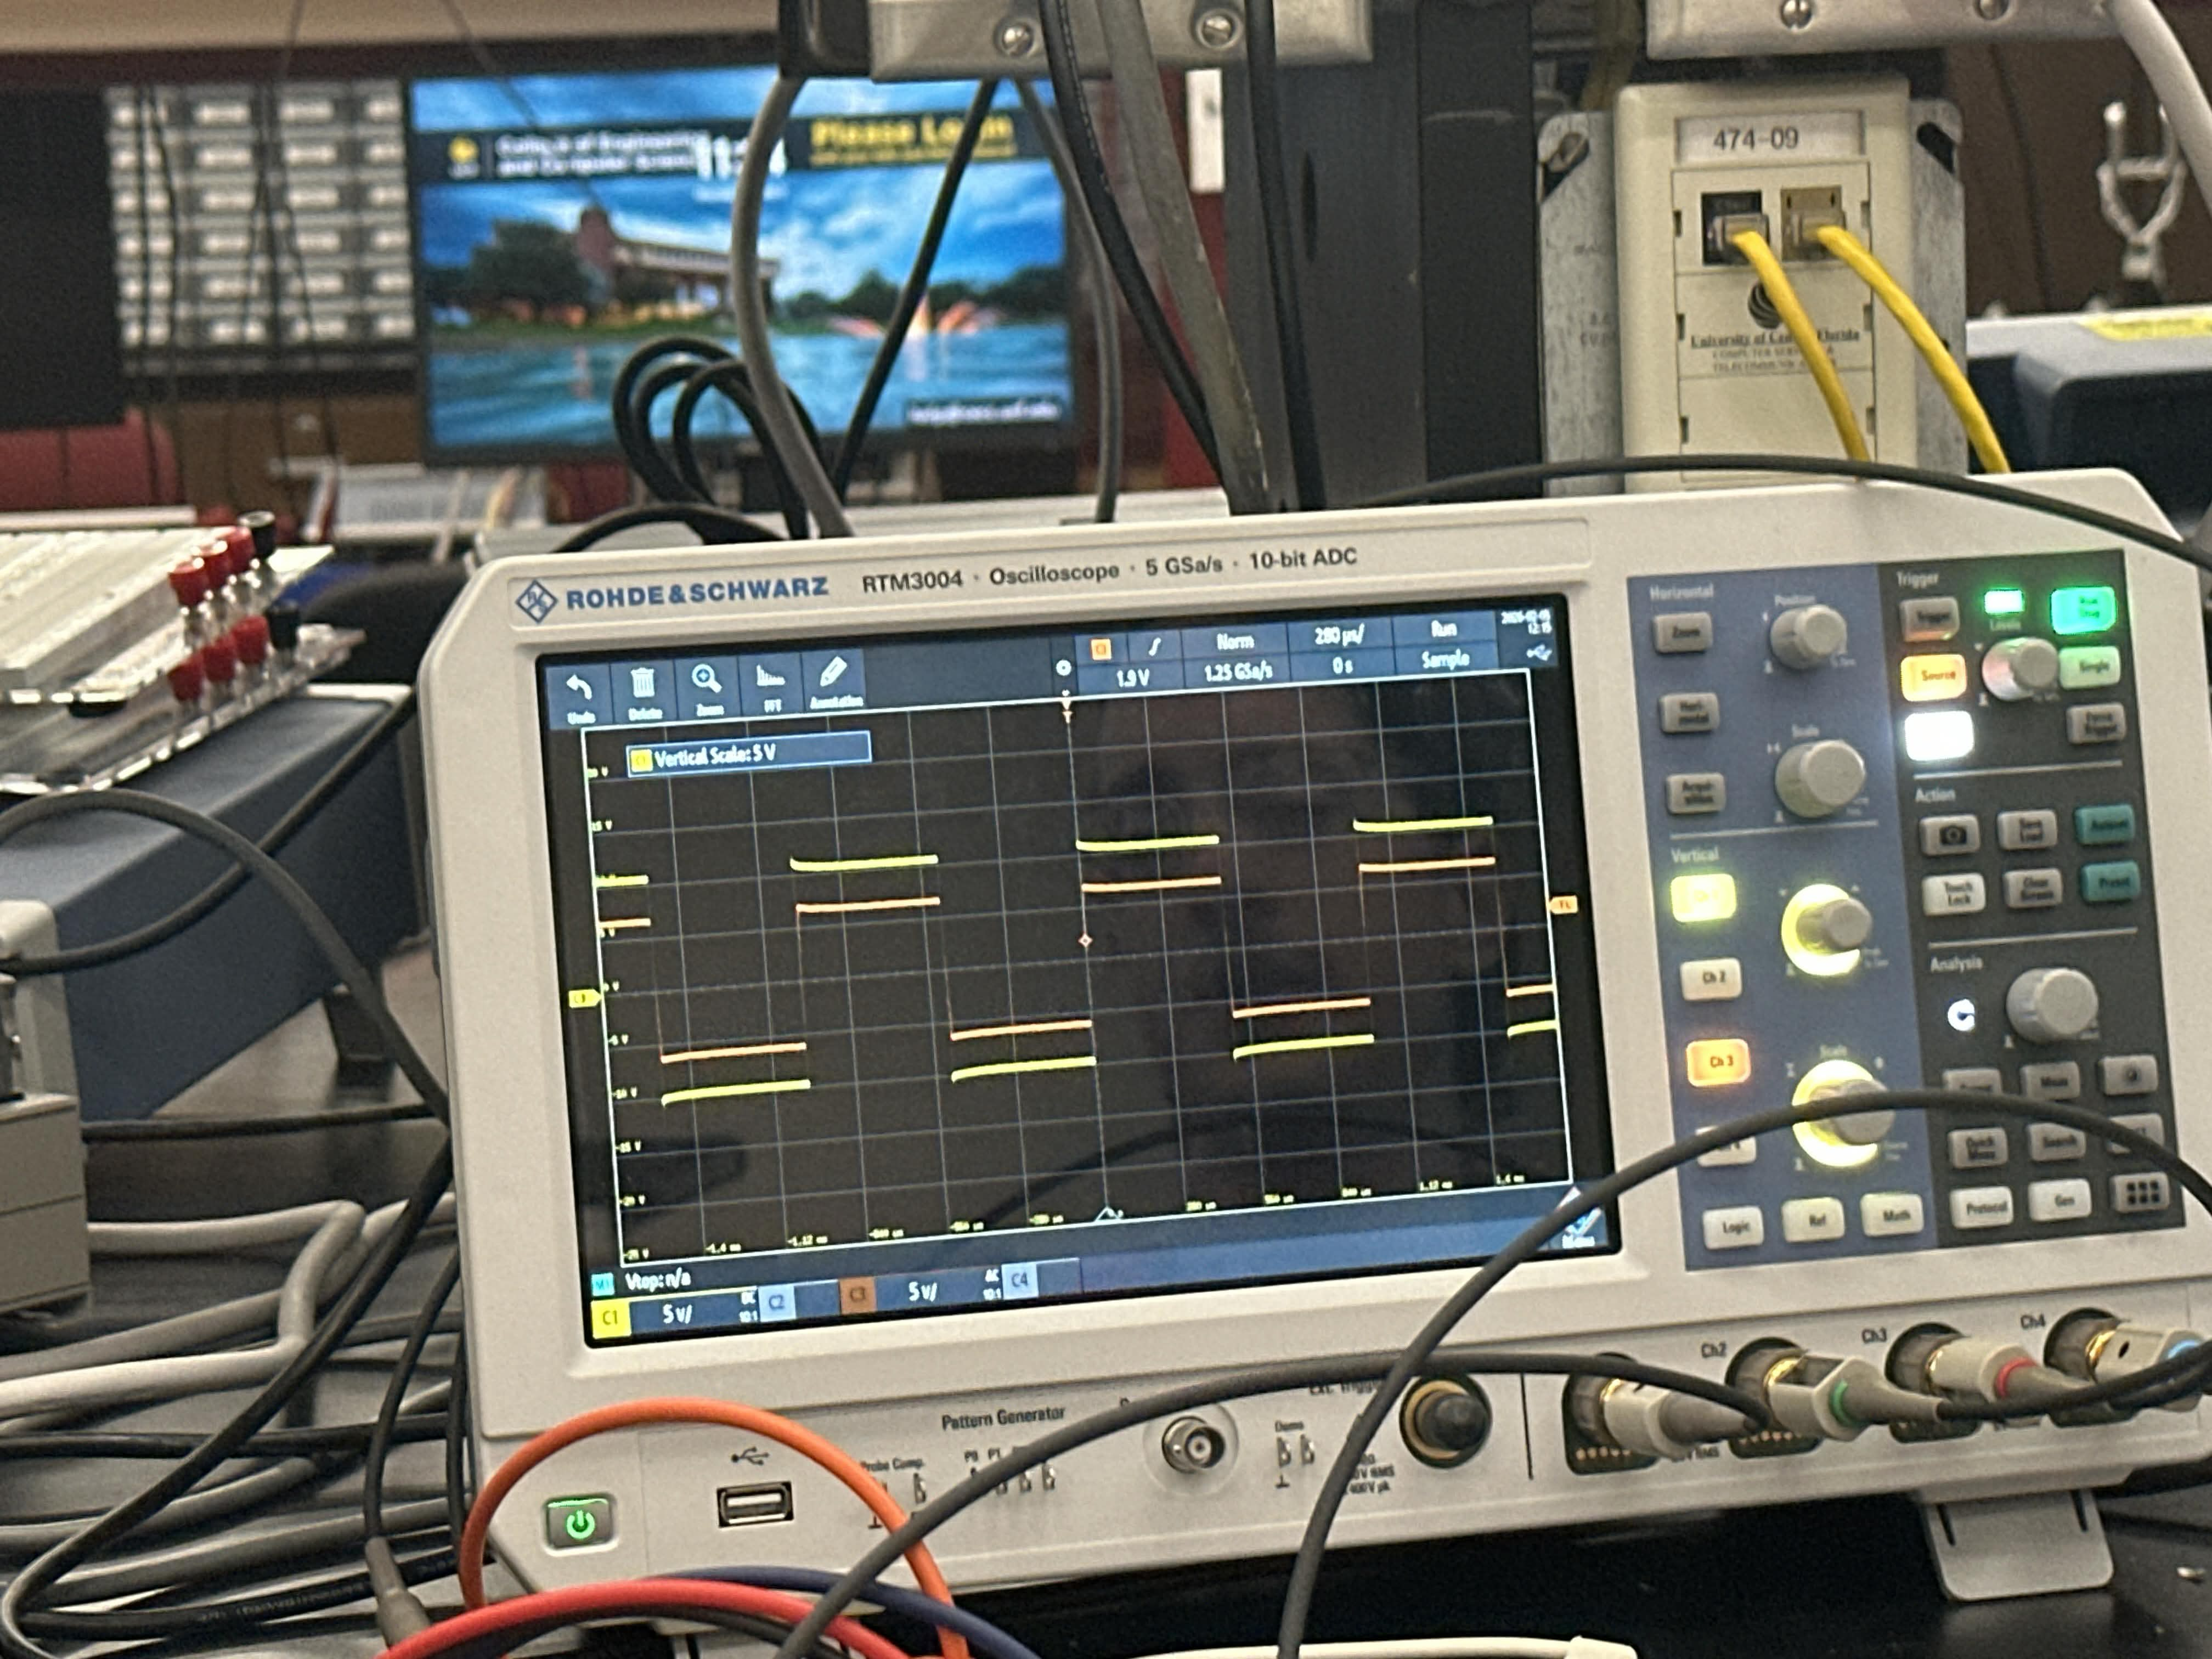
\includegraphics[width=\textwidth]{figure4_square.jpg}
		\caption{Square Input (Blue) vs Output (Yellow)}
		\label{fig:zener_square}
	\end{subfigure}
	\caption{Oscilloscope captures for the Zener clipping circuit.}
	\label{fig:zener_results}
\end{figure}

\textbf{Discussion:} \\
The back-to-back Zener diode configuration clips the output symmetrically on both half-cycles:
\begin{itemize}
	\item \textbf{Positive Clipping:} One Zener diode is forward-biased ($\approx 0.65\,\text{V}$) while the other is in Zener breakdown ($\approx 6.2\,\text{V}$), limiting the positive output to approximately $V_Z + V_{on} \approx 6.85\,\text{V}$.
	\item \textbf{Negative Clipping:} The roles of the two diodes reverse, and the negative output is similarly limited to approximately $-6.85\,\text{V}$.
	\item The flat tops and bottoms visible on the sinusoidal output in Figure~\ref{fig:zener_sine} confirm the symmetric clipping.
\end{itemize}

\textbf{Calculation:}
The Zener clipping threshold is:
\[
V_{clip} = V_Z + V_{on} = 6.2 + 0.65 = 6.85\,\text{V}
\]
The input was set to $20\,\text{V}_{pp}$ ($V_p = 10\,\text{V}$) to ensure the amplitude was sufficiently larger than $V_{clip}$. When the input amplitude was varied, the amount of clipping changed accordingly: at lower amplitudes ($V_p < 6.85\,\text{V}$) no clipping was observed, while at higher amplitudes the flat-topped waveform became progressively wider.

%-----------------------------------------
% CLAMPING CIRCUIT (Lab Manual Fig. 5)
%-----------------------------------------
\subsection{Clamping Circuit (Lab Manual Fig.~5)}
The dedicated clamping circuit (Lab Manual Fig.~5) shifts the DC level of the entire input signal without distorting its shape. The RC time constant was selected to be approximately $\tau = RC \approx 0.2\,\text{s}$.

\begin{figure}[H]
	\centering
	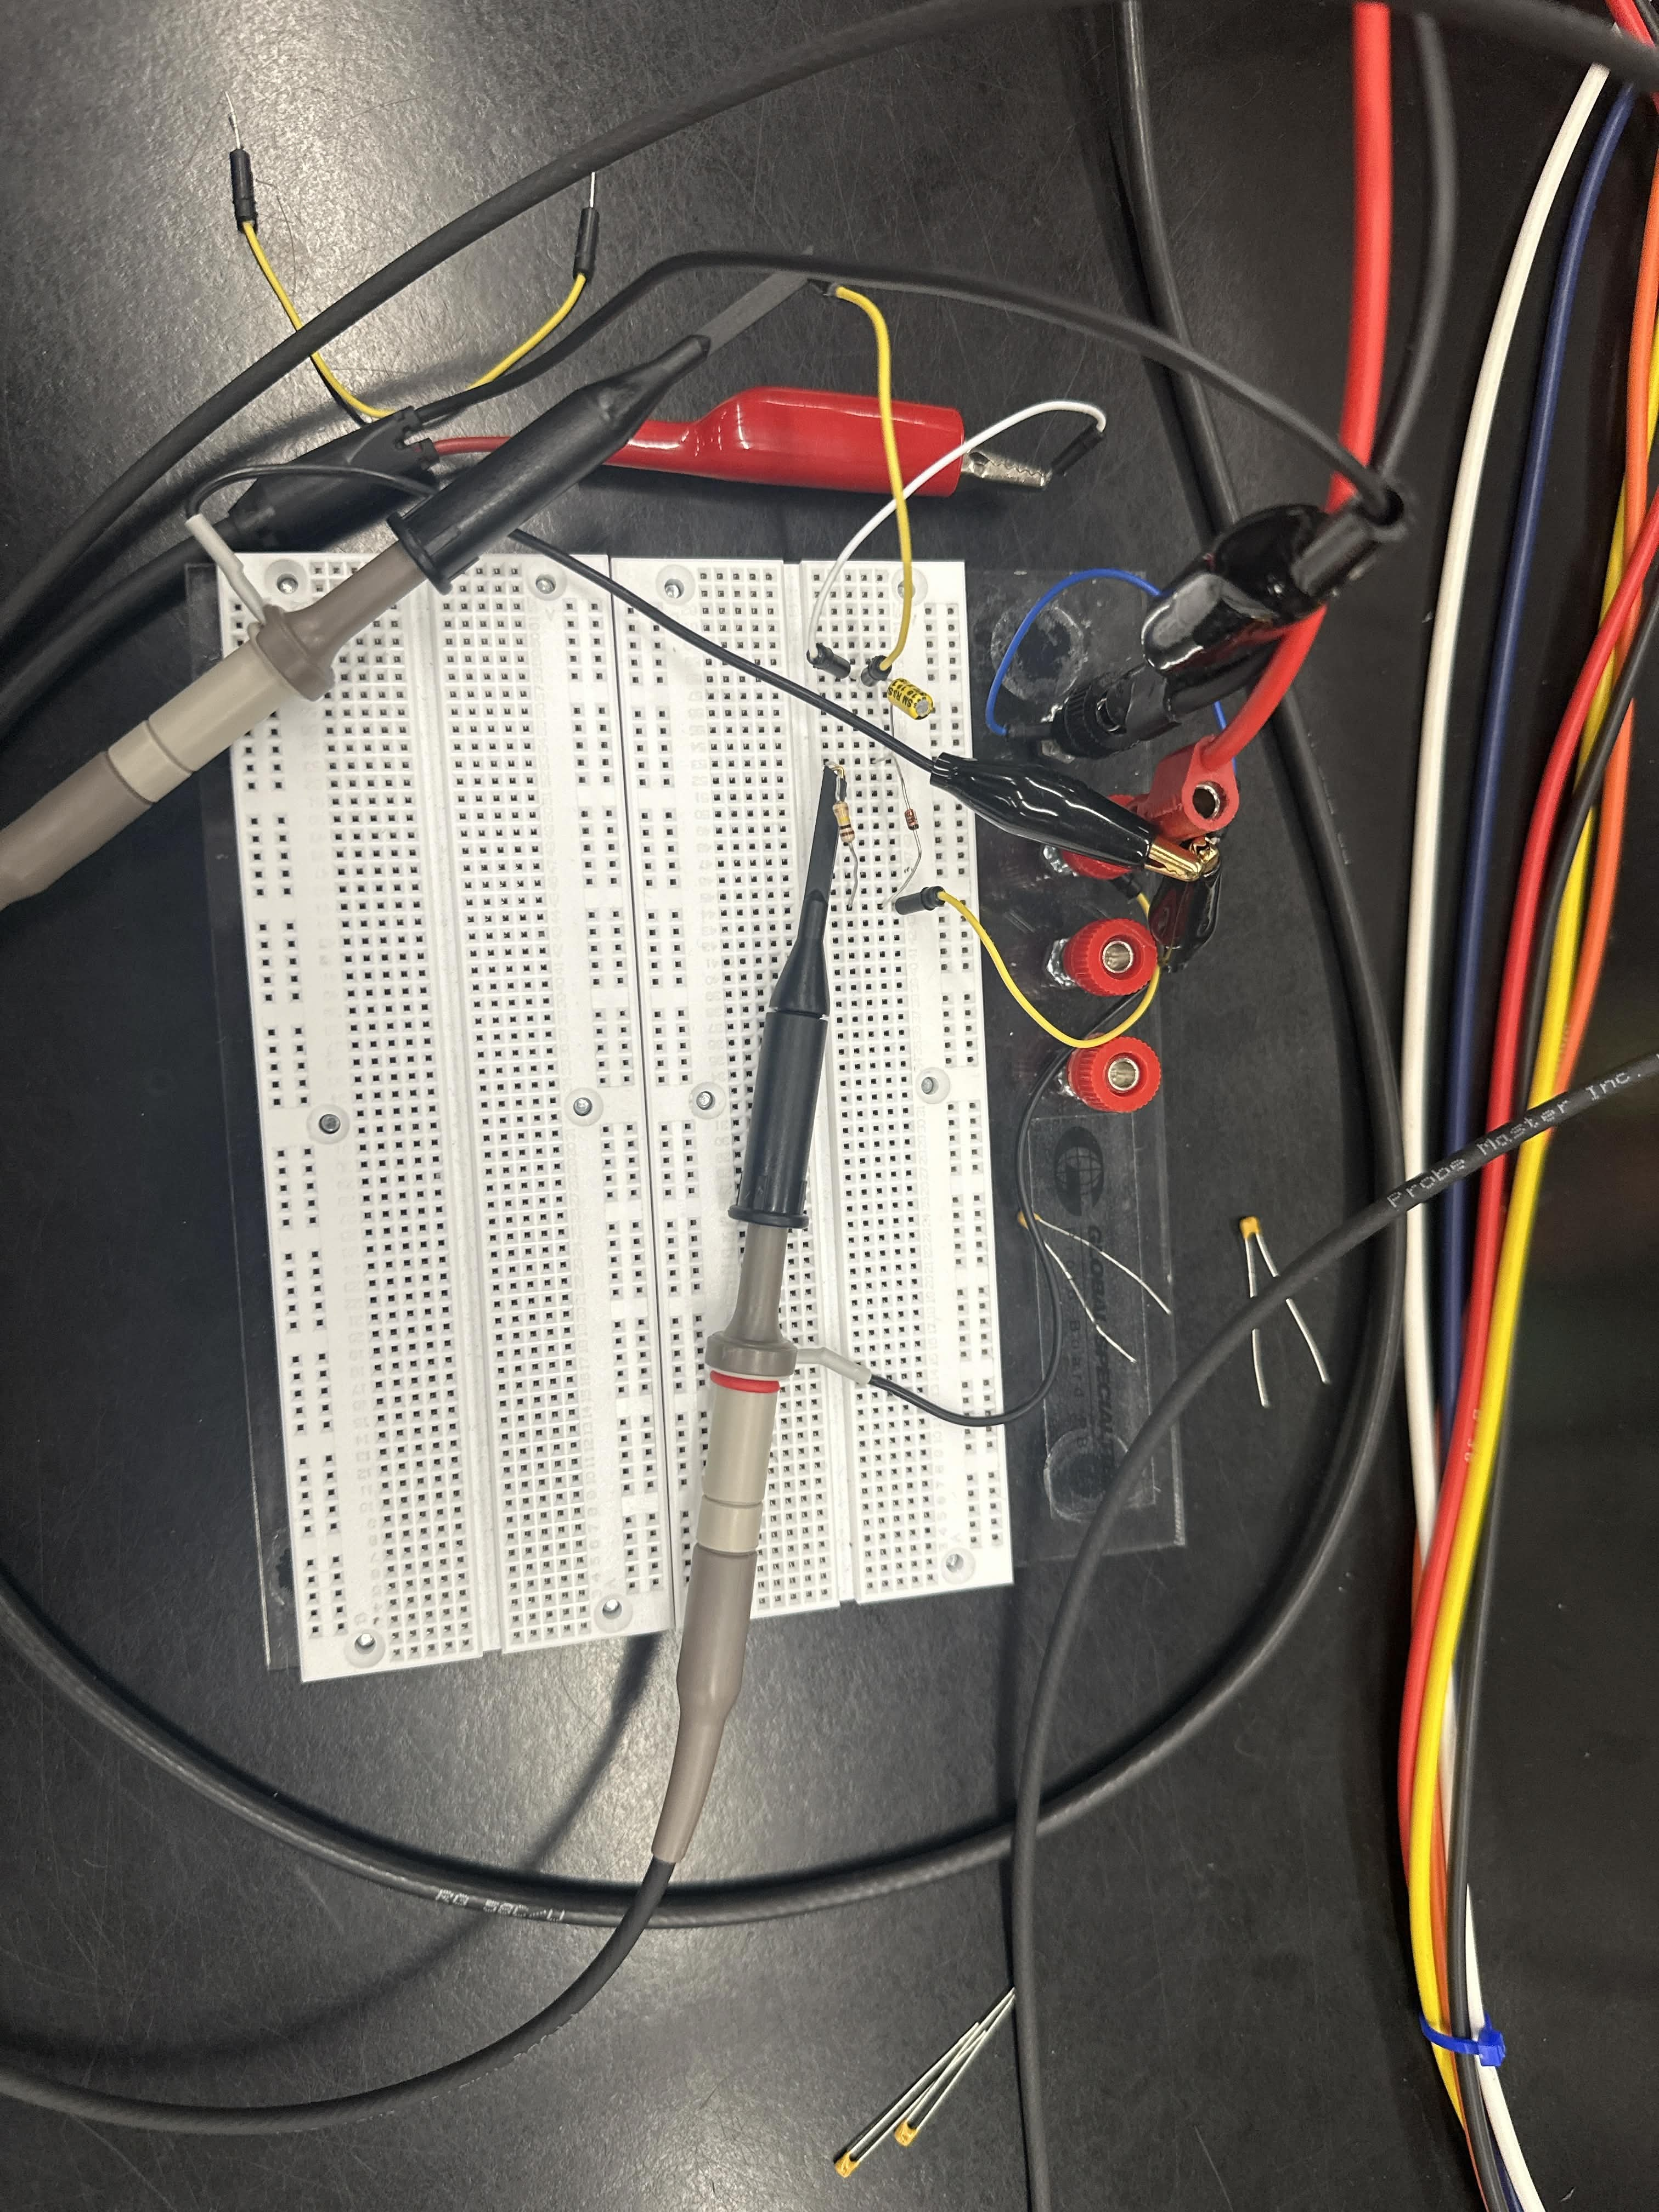
\includegraphics[width=0.6\textwidth,angle=90]{figure5.jpg}
	\caption{Breadboard of the clamping circuit.}
	\label{fig:hand_drawn_5}
\end{figure}

\begin{figure}[H]
	\centering
	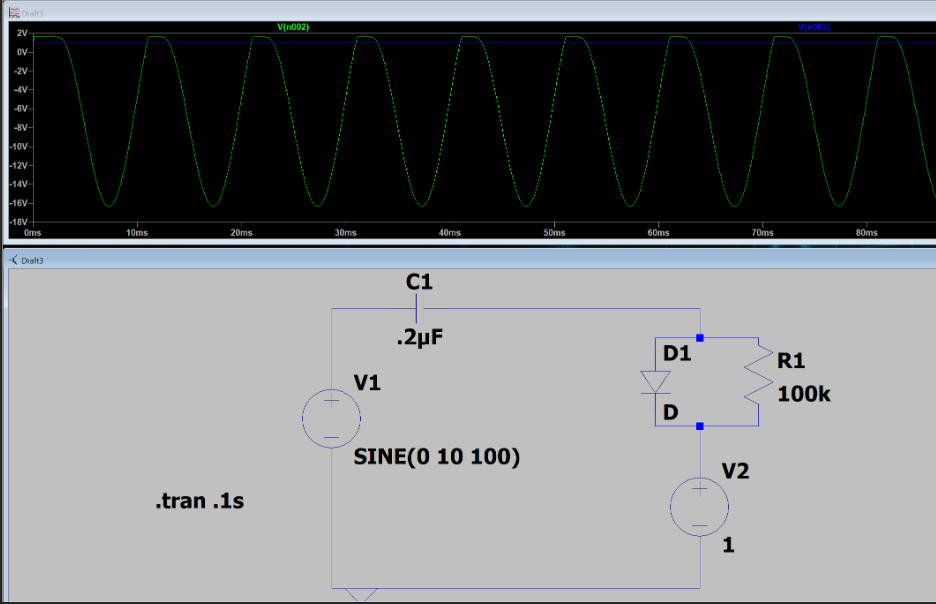
\includegraphics[width=0.6\textwidth]{figure5_ltspice.png}
	\caption{LTspice simulation schematic for the clamping circuit.}
	\label{fig:clamp5_sch}
\end{figure}

\begin{figure}[H]
	\centering
	\begin{subfigure}[b]{0.48\textwidth}
		\centering
		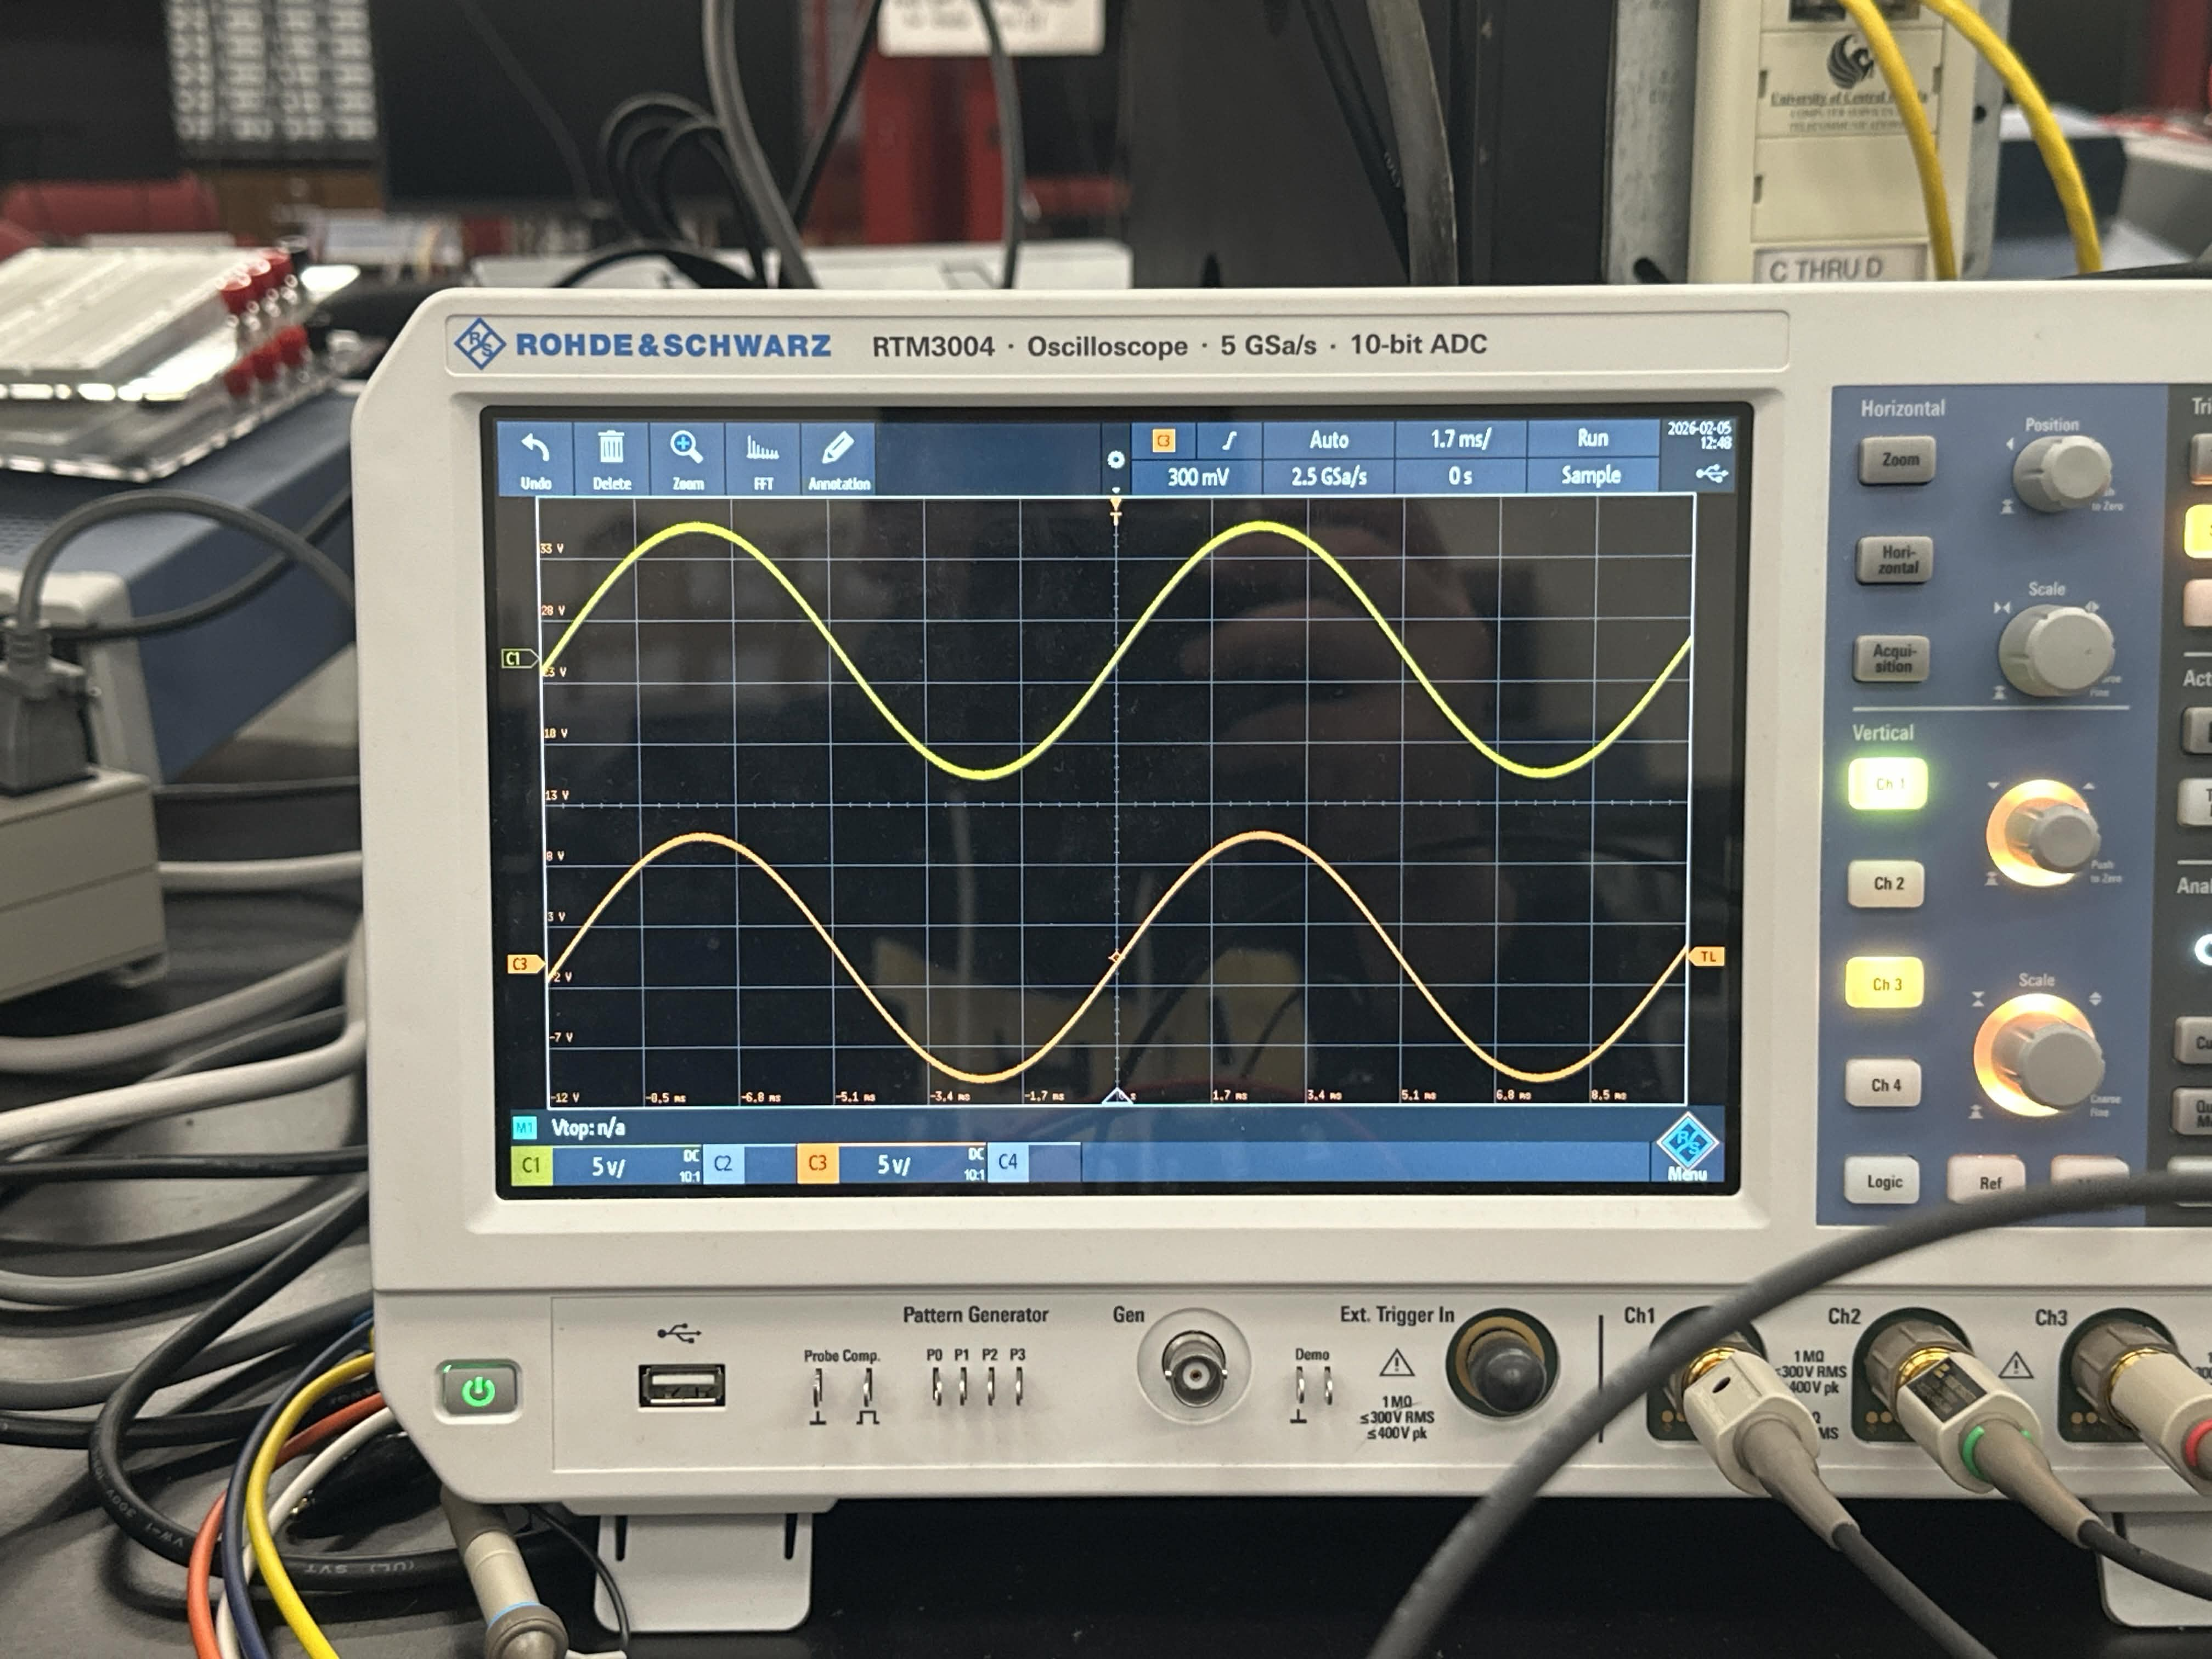
\includegraphics[width=\textwidth]{figure5_sine.jpg}
		\caption{Sinusoidal Input (Blue) vs Output (Yellow)}
		\label{fig:clamp5_sine}
	\end{subfigure}
	\hfill
	\begin{subfigure}[b]{0.48\textwidth}
		\centering
		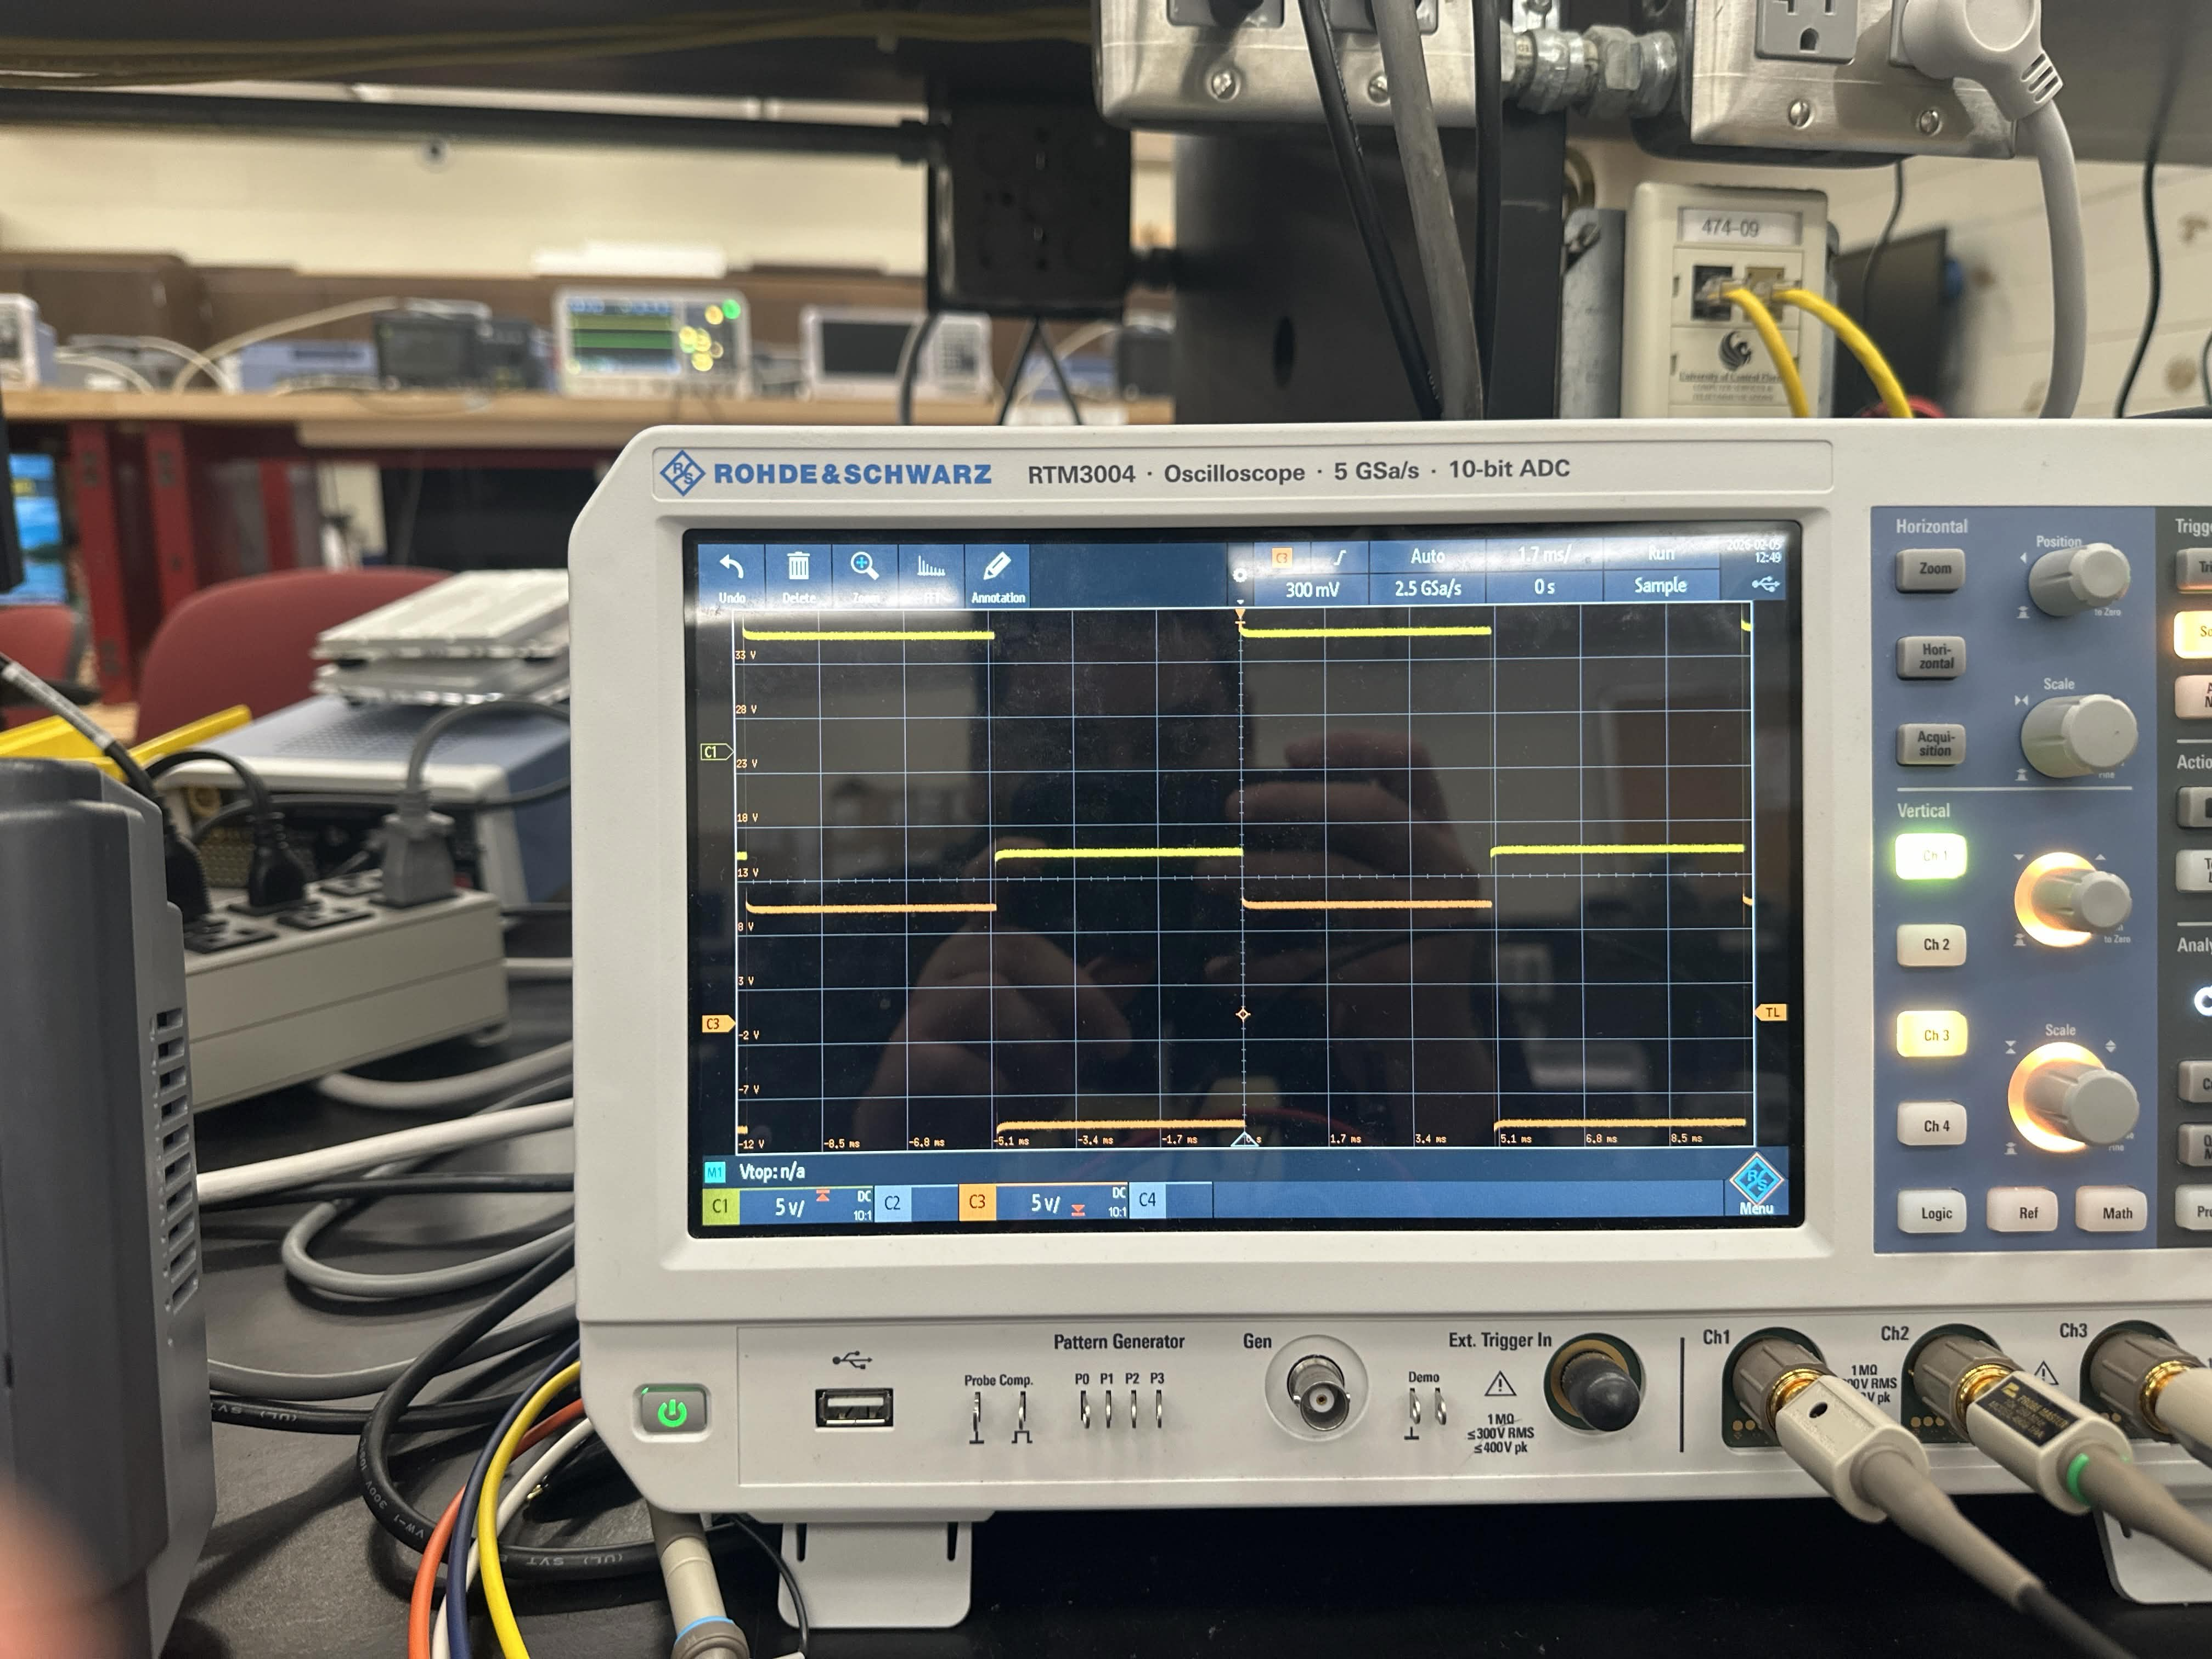
\includegraphics[width=\textwidth]{figure5_square.jpg}
		\caption{Square Input (Blue) vs Output (Yellow)}
		\label{fig:clamp5_square}
	\end{subfigure}
	\caption{Oscilloscope captures for the clamping circuit (Lab Manual Fig.~5).}
	\label{fig:clamp5_results}
\end{figure}

\textbf{Discussion:} \\
The clamping circuit shifts the entire waveform without altering its shape:
\begin{itemize}
	\item The capacitor charges through the forward-biased diode during the first applicable half-cycle, storing a voltage of approximately $V_p - V_{on}$.
	\item Once charged, the capacitor acts as a DC voltage source in series with the input, effectively shifting the waveform so that its peaks (or troughs) are clamped to the diode's forward voltage.
	\item The large $RC$ time constant ensures minimal discharge of the capacitor between cycles, maintaining a stable DC shift.
	\item Figure~\ref{fig:clamp5_results} confirms that the output waveform retains the same shape and amplitude as the input but is shifted in DC level.
\end{itemize}

\textbf{Calculation:}
With $R = 20\,\text{k}\Omega$ and $C = 10\,\mu\text{F}$ ($\tau = RC = 0.2\,\text{s}$), the capacitor charges to:
\[
V_C = V_p - V_{on}
\]
For $V_p = 5\,\text{V}$, the DC shift is $\Delta V_{DC} = 5.0 - 0.65 = 4.35\,\text{V}$, resulting in:
\[
V_{out,\text{min}} \approx -0.65\,\text{V}, \qquad V_{out,\text{max}} \approx 2(5.0) - 0.65 = 9.35\,\text{V}
\]

\textbf{Effect of amplitude variation:} When the input amplitude was varied, the clamping circuit adjusted its DC shift accordingly. The capacitor re-charged to the new peak value, and the output waveform always maintained its most negative excursion near $-V_{on}$.

\textbf{Effect of DC offset:} When a DC offset was added to the input using the function generator's offset control, the clamping circuit absorbed the offset. The capacitor charged to a new equilibrium, and the output remained clamped at the same reference level regardless of the input DC content. This confirms the clamper's role as a DC restorer.

%----------------------------------------------------------------------------------------
%	4. CONCLUSION
%----------------------------------------------------------------------------------------
\section{Conclusion}

\subsection*{Summary of Observations}
This experiment investigated the non-linear properties of PN junction diodes across five circuit configurations. The key quantitative observations are summarized below:
\begin{itemize}
	\item The \textbf{half-wave rectifier} (no capacitor) produced a peak output of approximately $V_p - V_{on} = 4.3\,\text{V}$ for a $5\,\text{V}$ peak input, confirming the expected $0.7\,\text{V}$ diode drop. The negative half-cycle was completely blocked, consistent with the piecewise-linear transfer characteristic.
	\item The \textbf{full-wave rectifier} doubled the output frequency to $200\,\text{Hz}$, and the experimental waveforms closely matched the theoretical $V_{out} = |V_{in}| - V_{on}$ transfer characteristic.
	\item The \textbf{half-wave peak rectifier} produced a near-DC output with a calculated ripple of $V_{r(pp)} \approx 0.215\,\text{V}$ (approximately $5\%$ of $V_p$). The \textbf{full-wave peak rectifier} reduced the ripple to $\approx 0.1075\,\text{V}$, confirming the expected factor-of-two improvement.
	\item The \textbf{clipping circuit} limited the output at $V_{ref} + V_{on}$, and the \textbf{Zener clipper} provided symmetric clipping at $\pm(V_Z + V_{on}) \approx \pm 6.85\,\text{V}$. Varying the input amplitude confirmed the onset and widening of the clipped region.
	\item The \textbf{clamping circuit} shifted the entire waveform by $V_p - V_{on}$ without distortion. Adding a DC offset to the input did not affect the clamped reference level, confirming its DC-restoring capability.
\end{itemize}
The experimental waveforms were consistent with the pre-lab calculations and LTspice simulations across sinusoidal, square, and triangular inputs. Minor discrepancies in the exact diode voltage drop (measured $\approx 0.6$--$0.7\,\text{V}$ vs.\ the ideal $0.7\,\text{V}$) are attributed to device-to-device variation and temperature effects.

\subsection*{What I Learned}
This experiment reinforced several important concepts beyond the textbook theory:
\begin{itemize}
	\item I gained hands-on appreciation for the \textbf{non-ideal diode drop}: the forward voltage varies slightly with current and temperature, which explains the small differences between simulation and bench measurements.
	\item The \textbf{RC time constant} directly controls the quality of the filtered DC output. By computing $\tau = 0.2\,\text{s}$ and observing the resulting ripple, I saw how the interplay between capacitor size and load resistance determines power supply performance in practice.
	\item Working with the \textbf{clamping circuit} taught me that the capacitor ``remembers'' the peak voltage and acts as a DC battery---an insight that clarified how DC restorers function in communication receivers.
	\item Using the oscilloscope in \textbf{differential mode} for the full-wave rectifier was a practical skill I had not used before. Understanding why the shared ground between the scope and function generator necessitates differential measurement deepened my understanding of instrumentation.
	\item Overall, this experiment demonstrated that simple combinations of passive components and diodes can perform sophisticated signal processing tasks---rectification, clipping, and clamping---that are foundational to analog circuit design.
\end{itemize}

\end{document}
